%\documentclass[handout,ignorenonframetext,red]{beamer}
\documentclass[ignorenonframetext,red]{beamer}
%\documentclass[class=article, a4paper]{beamer}
%\documentclass[handout]{beamer} %pour sortie papier


\usepackage[french]{babel}
\usepackage{pgf,pgfarrows,pgfn odes,pgfautomata,pgfheaps,pgfs hade}
\usepackage{amsmath,amssymb}
\usepackage[utf8]{inputenc}
\usepackage{stmaryrd}
\usepackage{url}


%\documentclass[svgnames,ignorenonframetext]{beamer}
%\usepackage{times}
\usepackage{listings}
\usepackage{amsmath,multicol}
\usepackage{verbatim}
%\usepackage{beamerarticle}
\usepackage{longtable}
%\usepackage{ucs}
%\usepackage[utf8]{inputenc}
\usepackage{pdfpages}

\setcounter{tocdepth}{1}

\mode<presentation>
{
  \usetheme{Warsaw}
  \setbeamercovered{transparent}
  \AtBeginSection[]
  {
    \begin{frame}<beamer>
       \setcounter{tocdepth}{2}
       \tableofcontents[currentsection,currentsubsection,hideothersubsections]
    \end{frame}
  }

  \AtBeginSubsection[]
  {
    \begin{frame}<beamer>
    \frametitle{\thesection. \insertsectionhead}
       \tableofcontents[sectionstyle=hide/hide,subsectionstyle=show/shaded/hide ]
    \end{frame}
  }
  
  \addtobeamertemplate{footline}{\insertframenumber/\inserttotalframenumber}

}

%\mode<handout>{  \setbeamercolor{background canvas}{bg=black!5}} }


\logo{\vspace{-.10cm} \includegraphics[scale=0.1]{../illustration/logo_cnam.png}}
\date{\today}
\author{Rémi LEBLOND\\ \url{http://remileblond.fr/SMB137}}
\institute{Conservatoire National des Arts et Métiers - Centre de Strasbourg}



\title{SMB137 - Première partie}
\subtitle{Historique et principes de base}

\begin{document}

\frame[plain]{\titlepage}

\begin{frame}
 \frametitle{Plan} 
 \tableofcontents
\end{frame} 

\begin{frame}
 \frametitle{Qu'est-ce qu'un système informatique ?}

  \begin{definition}
Ensemble constitué d'un ou de plusieurs ordinateurs, de périphériques et de logiciels, et qui assure le traitement des données.

\textit{[AFNOR]}
\end{definition}
But :
\begin{itemize}
\item Traiter des données (exécuter des programmes)
\end{itemize}
 \end{frame} 
 

\section{Historique - Grandes familles de systèmes}
\subsection{Les premiers systèmes}
%------------------------------------------------------------------- 

\begin{frame}{Les calculateurs mécaniques}
\begin{itemize}
\item <1> Machine de Pascal (1642) :
\begin{itemize}
\item Entièrement mécanique
\item Additions et des soustractions.
\end{itemize}
\item <2> Machine de Gottfried Wilhelm (1672) :
\begin{itemize}
\item Multiplications et des divisions
\end{itemize}
\item <3> Charles Babbage (1792 - 1871) : la \textbf{machine analytique}
\begin{itemize}
\item 
\begin{tabbing}
Quatre éléments : \= Le magasin \= $\rightarrow$ la mémoire \\
\>Le moulin \> $\rightarrow$ unité de calcul \\
\>L'entrée \> $\rightarrow$ lecteur de carte \\
\>La sortie \> $\rightarrow$ impression par perforation
\end{tabbing}
\item Exécution d'algorithmes simples décrits sur carte perforée
\item Très (trop\footnote{Terminée après sa mort, par un de ses fils, en 1910.}) complexe, mais visionnaire. A vapeur !
\end{itemize}
\end{itemize}
\end{frame}

\begin{frame}{La machine analytique de Babbage}
\begin{figure}
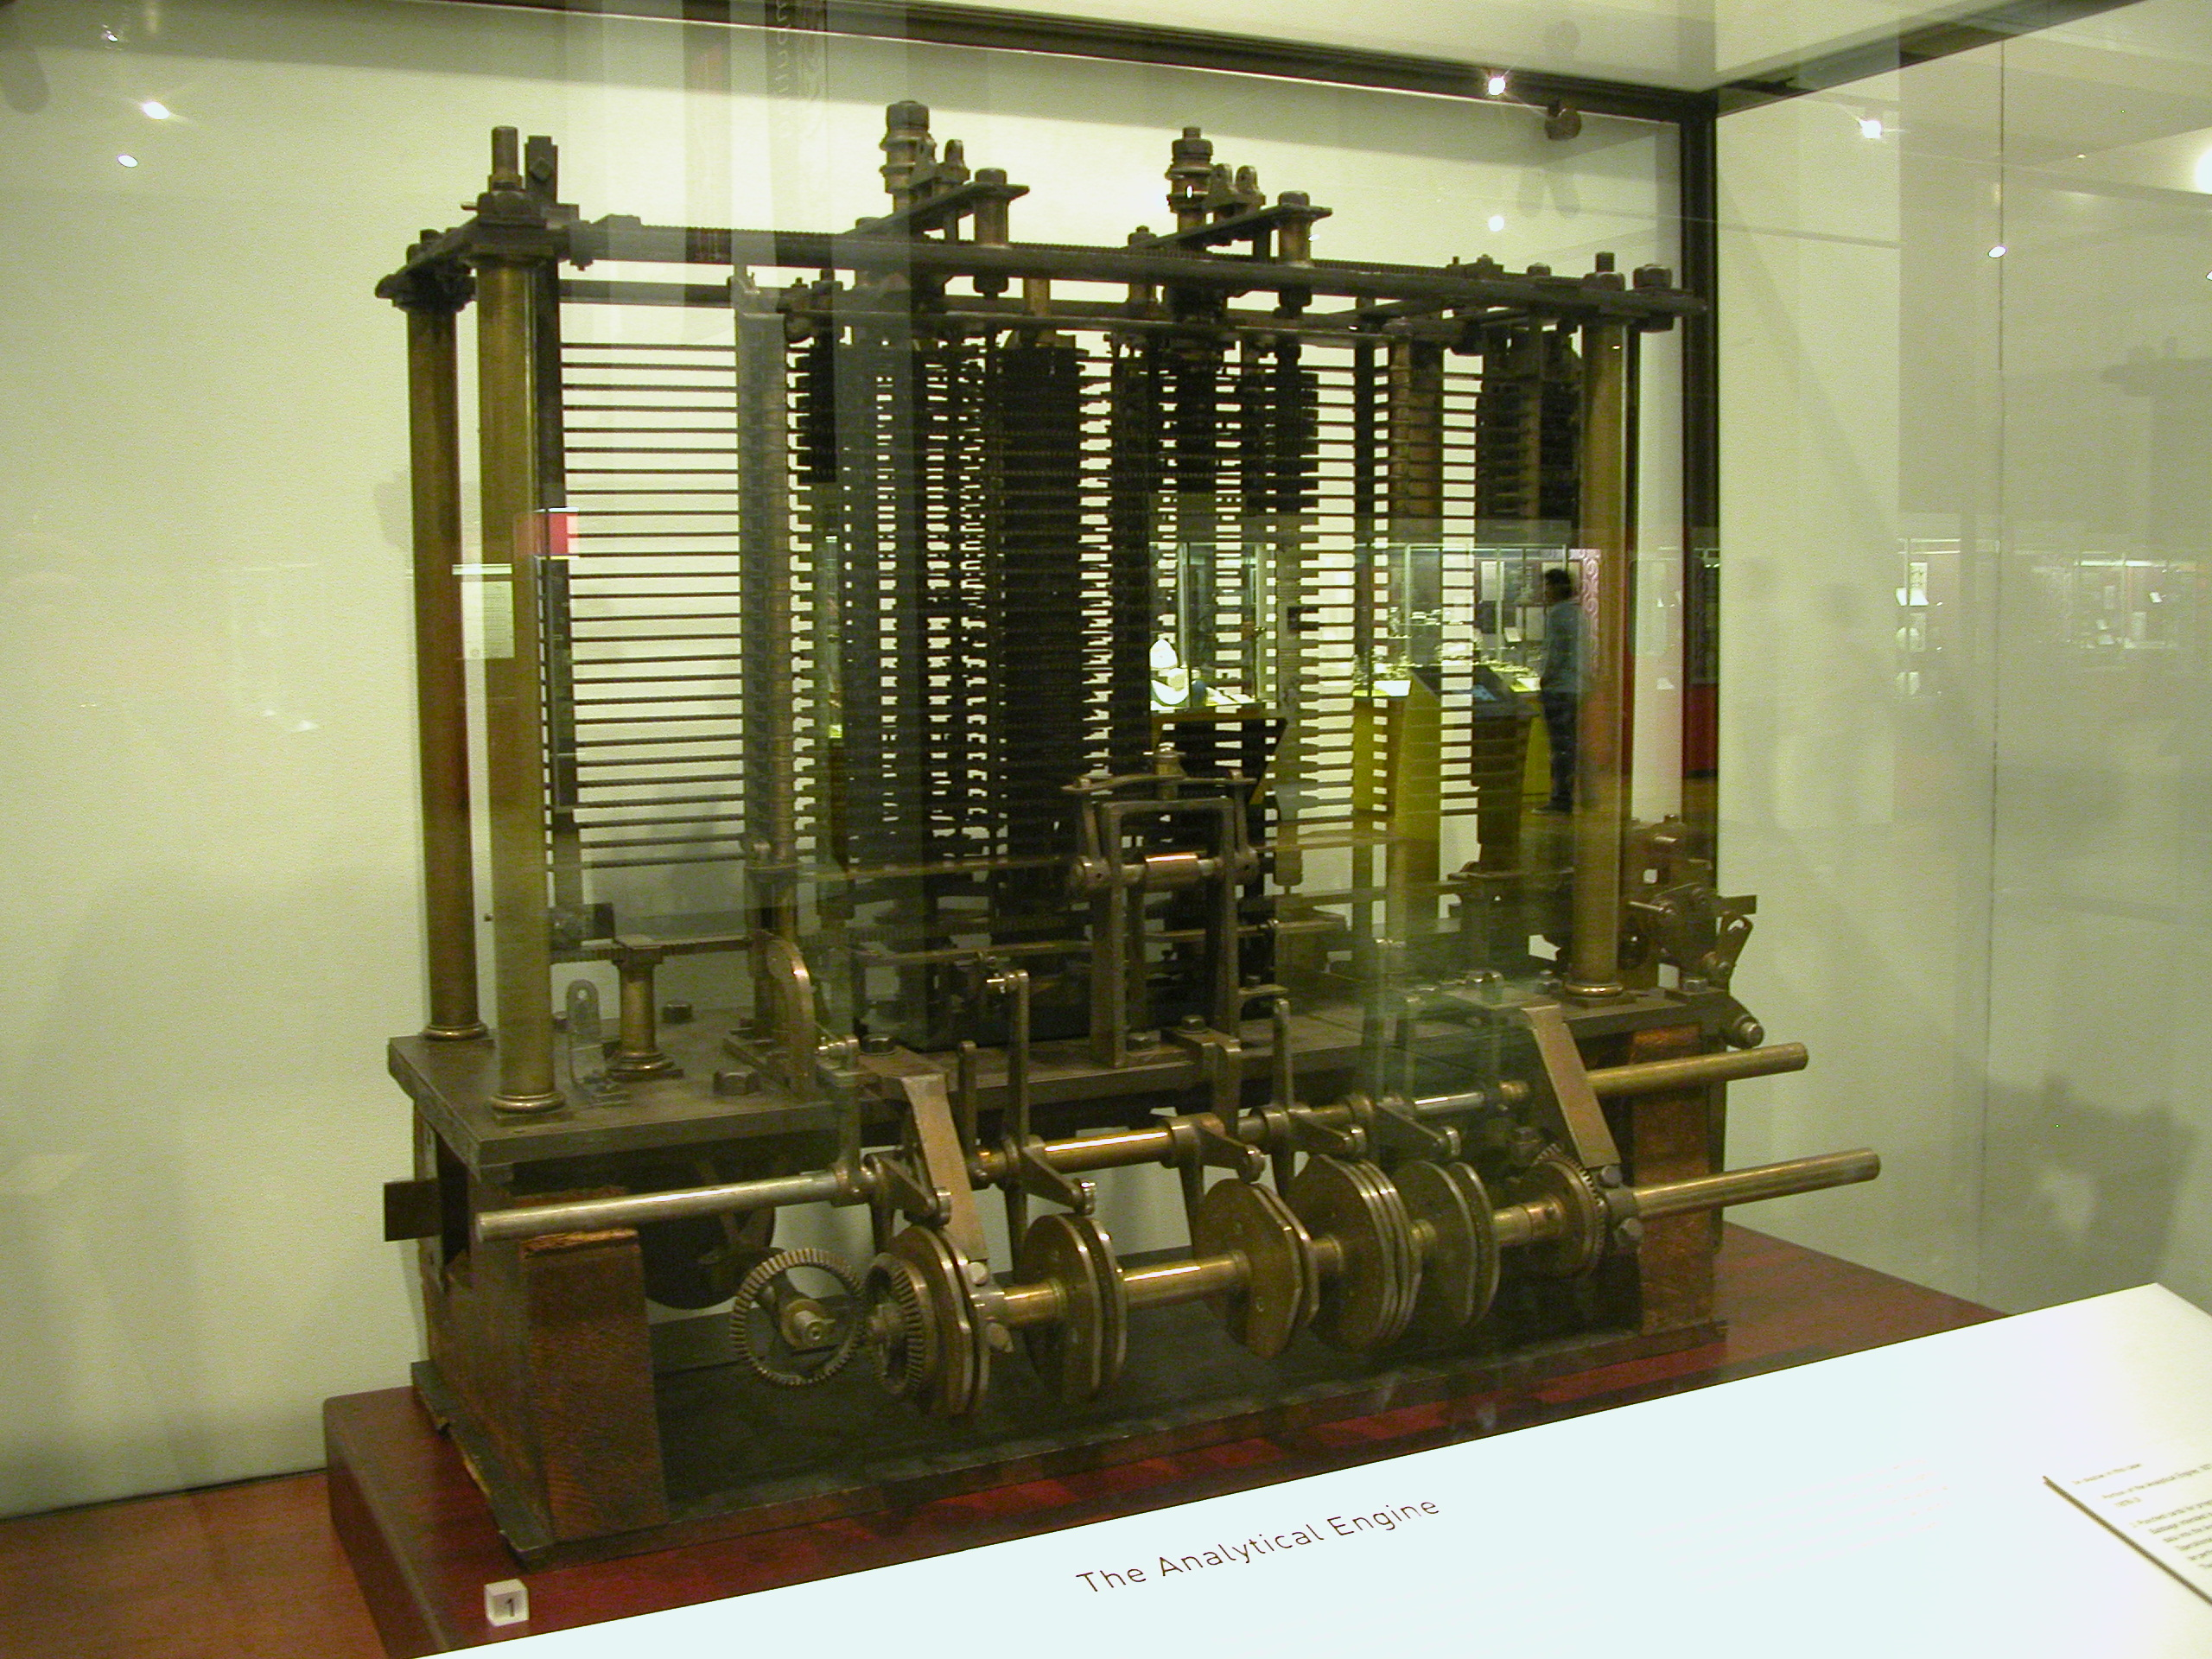
\includegraphics[height=5cm]{../illustration/AnalyticalMachine_Babbage_London.jpg}
\caption{Prototype (1871) non terminé de la machine analytique de Babbage, exposée au Science Museum de Londres \cite{wp-mab}.}
\end{figure}
\end{frame}

\begin{frame}{Systèmes basés sur des relais électromécaniques}
\begin{itemize}
\item<1> Z1 (1938), Z2 et Z3 (1941) : Konrad ZUSE \cite{wp-zuse}
\begin{itemize}
\item Premier calculateur binaire\footnote{Première implémentation de l'algèbre Booléenne.} à virgule flottante
\begin{itemize}
\item Electro-mécanique : 2 600 relais de téléphone, film perforé
\item Multiplication : 5 secondes
\item Premier langage de haut niveau (Plankalkül) $\rightarrow$ 2000 !
\end{itemize}
\item Détruit par les bombardements alliés. Déclinaisons militaires S1 et S2 (aéronautique et balistique) $\rightarrow$ URSS ?
\item Logique purement commerciale
\end{itemize}
\item<2> Mark1 (1944) : Howard AIKEN pour IBM
\begin{itemize}
\item 760 000 pièces électromécaniques
\begin{itemize}
\item Multiplication de deux nombres de 23 chiffres en 6 secondes
\item Addition, soustraction : $\frac{3}{10}$ seconde
\end{itemize}
\item Obsolète avant même son achèvement
\end{itemize}
\end{itemize}
\end{frame}

\begin{frame}{Systèmes basés sur des tubes à vide}
\begin{itemize}
\item<1> Colossus (1943) : Alan TURING
\begin{itemize}
\item Services secrets britanniques
\item Premier calculateur électronique numérique
\item Décryptage des messages (Enigma)
\item Secret défense durant 30 ans (impasse scientifique)
\end{itemize}
\item<2> ENIAC (1946) : ECKERT et MAUCHLY
\begin{itemize}
\item Tables d'ajustement des tirs d'artillerie
\item \textit{18 000 tubes, 30 tonnes, 1 500 relais, 6 000 commutateurs, 160 m$^2$, 140 KW}
\item Fin guerre : exploitation scientifique
\item Base de travail scientifique (John VON NEUMANN)
\end{itemize}
\end{itemize}
\end{frame}

\begin{frame}
\frametitle{Qu'est qu'un programme ?}
\begin{definition}
Un programme correspond à une séquence d'instructions décrivant la façon dont une tâche doit être effectuée. \cite{tanen}
\end{definition}
\begin{itemize}
\item Décomposé en \textbf{opérations élémentaires}, pouvant être exécutées par les circuits de l'ordinateur :
\begin{itemize}
\item Additionner deux nombres
\item Tester si un nombre est égal à zéro
\item Copier une donnée d'un emplacement mémoire à un autre
\end{itemize}
\end{itemize}
\end{frame}


\begin{frame}{Programmation des premiers systèmes}
\begin{itemize}
\item Modules de traitement
\begin{itemize}
\item Inverseurs
\item Additionneurs
\item Portes logiques
\item ...
\end{itemize}
\item Câbles de liaison
\item Programmation
\begin{itemize}
\item Assemblage de modules
\item Câblage
\item Programmation par fiches et interrupteurs
\item Action directe sur le matériel
\end{itemize}
\end{itemize}
\end{frame}

\begin{frame}{ENIAC - 1946}
\includegraphics<1>[height=5cm]{../illustration/eniac1.png}
\includegraphics<2>[height=5cm]{../illustration/eniac2.png}
\end{frame}


\begin{frame}{Les premiers programmes autonomes}
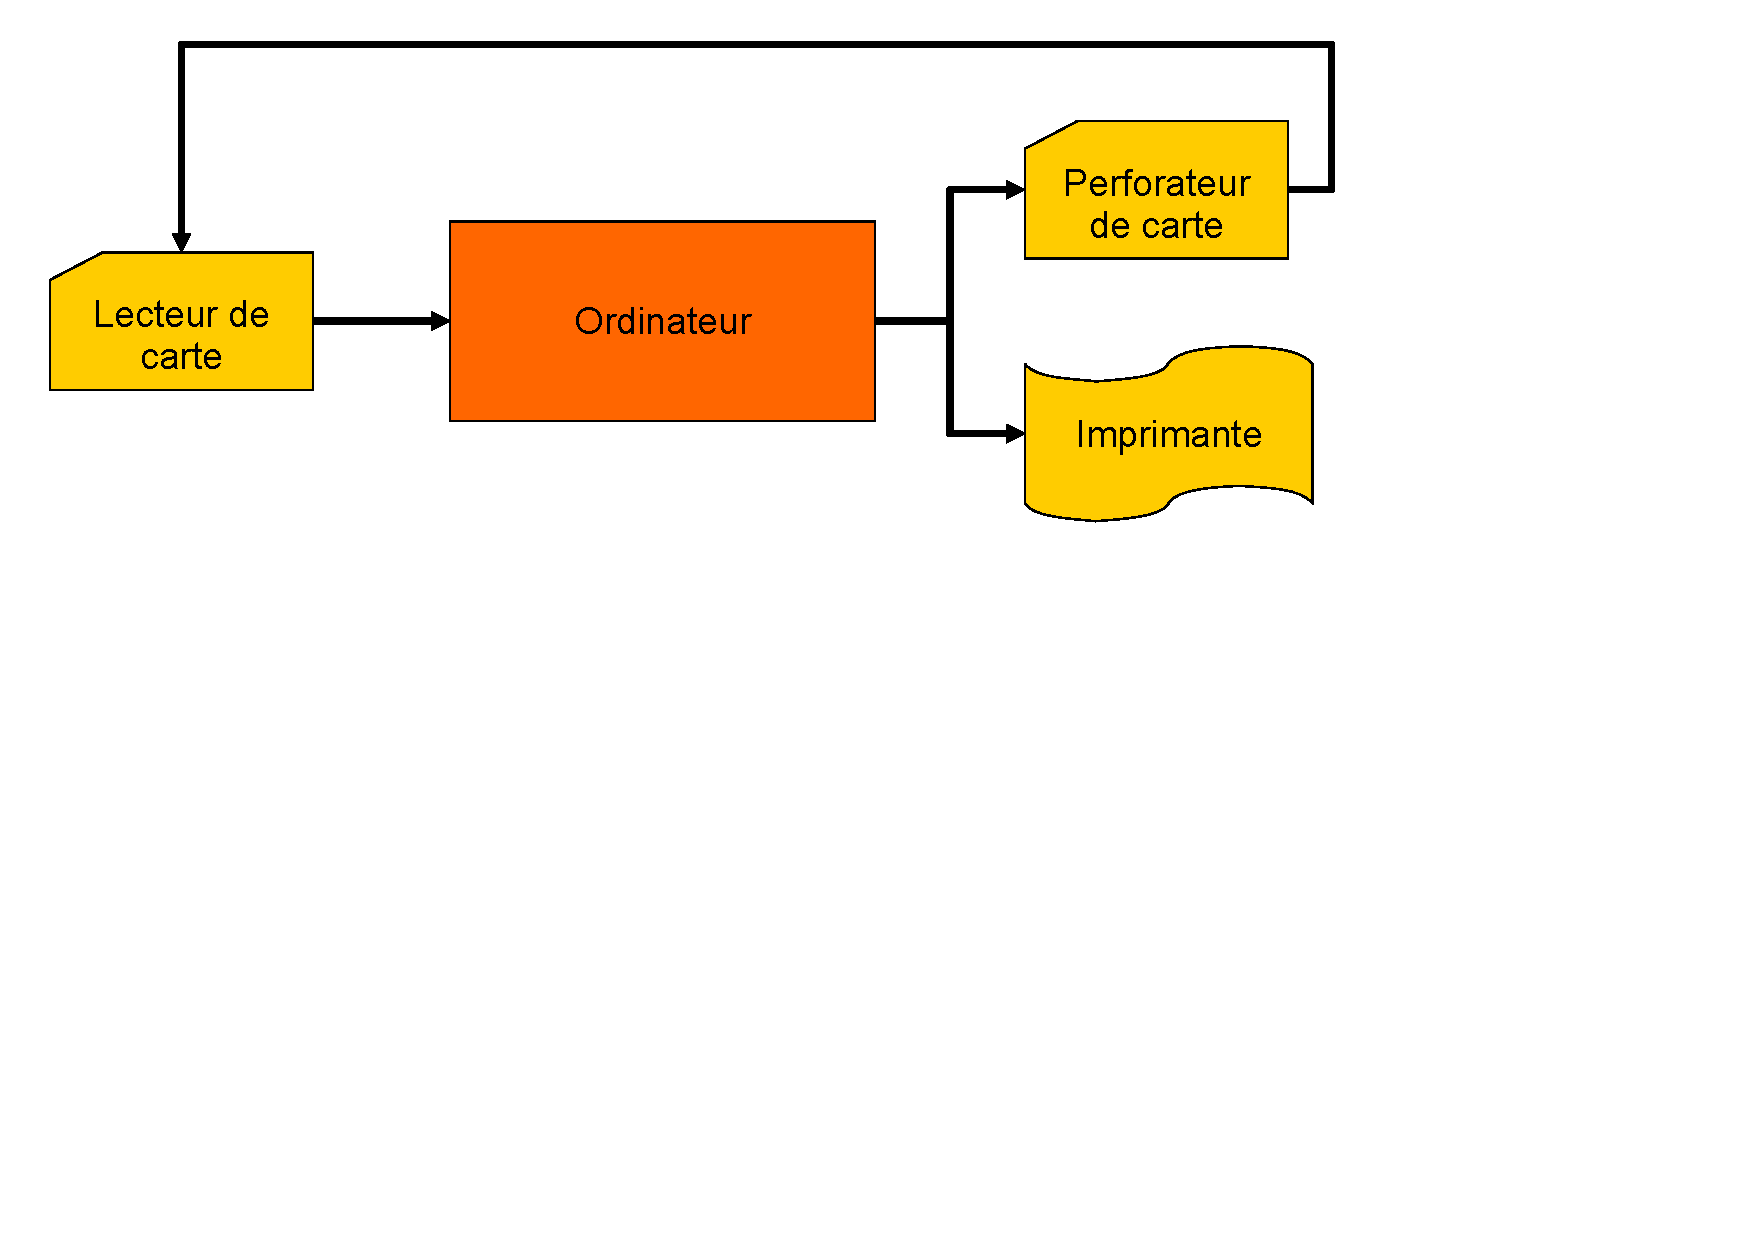
\includegraphics[height=4cm]{../illustration/pgm_autonome.pdf}
\end{frame}


\begin{frame}{L’ENIAC en 1957}
\begin{itemize}
\item Bilan d'une année de production
\item 7 247 heures de fonctionnement
\begin{itemize}
\item 3 491 heures en production
\item 1 061 heures en "problèmes"
\item 196 heures d’inactivité
\item 651 heures d’interventions planifiées
\item 1 848 heures d’interventions non planifiées
\begin{itemize}
\item remplacement de tubes
\item ...
\end{itemize}
\end{itemize}
\item 19 000 tubes remplacés
\end{itemize}
\end{frame}



\begin{frame}{L'héritage des premiers systèmes}
\begin{itemize}
\item Des systèmes complexes
\begin{itemize}
\item lent
\item coûteux
\item sous-utilisation des ressources
\item complexe à utiliser
\item peu fiable
\end{itemize}
\item Reproductibilité des traitements
\item Base pour d'importants travaux de recherche
\end{itemize}
\end{frame}


\begin{frame}{Les premiers systèmes}
\begin{columns}
\column{.5\textwidth}\begin{block}{Avantages}
\begin{itemize}
\item Reproductibilité des traitements
\item Vitesse de calcul (relative)
\item Base de travail scientifique
\end{itemize}
\end{block}
\column{.5\textwidth}\begin{block}{Inconvénients}
\begin{itemize}
\item Faible débit
\item Matériel sous utilisé
\item Délais de manipulation des cartes
\item Pas de langage de commande
\end{itemize}
\end{block}
\end{columns}
\end{frame}

\begin{frame}{La machine de Turing \cite{wp-turing}}
\begin{itemize}
\item Alan Mathison Turing (23 juin 1912 - 7 juin 1954) 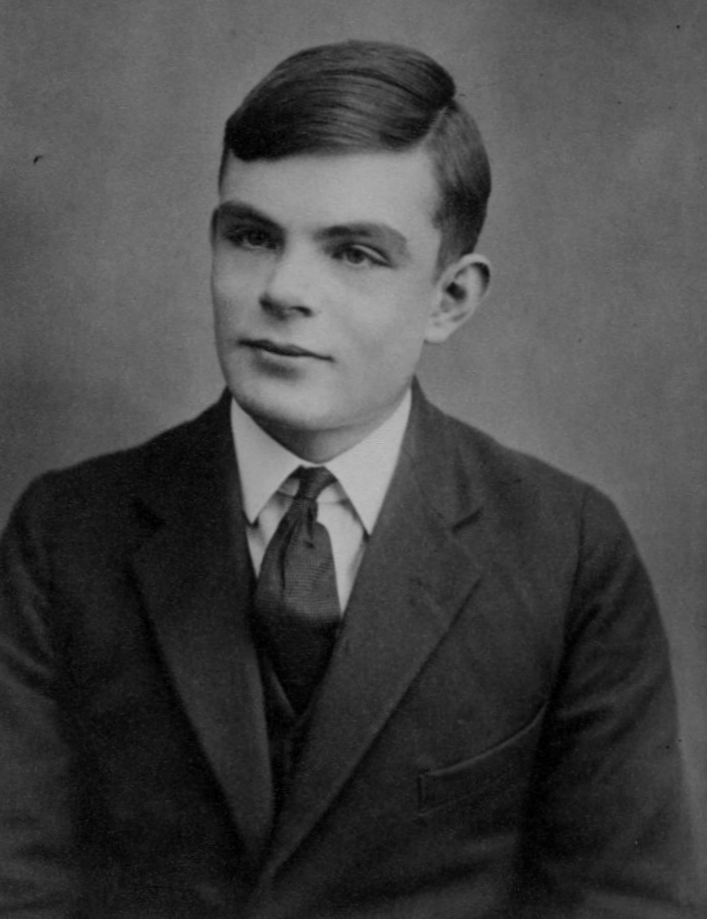
\includegraphics[height=1cm]{../illustration/Alan_Turing_Aged_16.jpg}
\begin{itemize}
\item Mathématicien, cryptologue et informaticien britannique
\item 1936 : article de logique mathématique
\begin{itemize}
\item problème de Hilbert dans les théories axiomatiques, le problème de la décision
\item solution « être calculant » : appareil logique ou humain bien discipliné appliquant des règles
\item fondements scientifiques de l'informatique.
\end{itemize}

\end{itemize}
\item Machine de Turing
\begin{itemize}
\item expérience de pensée
\item concepts de programmation et de programme
\item formalisation des concepts d'algorithme et de calculabilité
\end{itemize}

\end{itemize}

\end{frame}

\begin{frame}{La notion de logiciel \cite{wp-neumann}}
\begin{itemize}
\item Basée sur les travaux de John VON NEUMANN (1947) 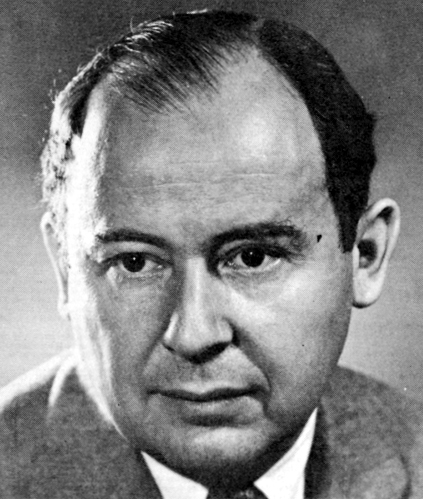
\includegraphics[height=1cm]{../illustration/JohnvonNeumann-LosAlamos.jpg}
\begin{itemize}
\item Description des traitements en mémoire et non plus directement dans le matériel
\item Chargement de la description des traitements en tant que données
\item Un appareil informatique est une machine qui effectue des traitements en fonction d'instructions et de données
\end{itemize}
\item Terme "logiciel" créé en 1972
\begin{itemize} 
\item Traduction de \textit{software} (par opposition au \textit{hardware})
\end{itemize}
\item Premiers langages de programmation
\begin{itemize}
\item description de traitements : enchaînement d'instructions
\end{itemize}
\end{itemize}

\end{frame}

\begin{frame}{Utilisation du transistor (1955-1965)}
\begin{itemize}
\item Laboratoires Bell 1948
\item Remplacement des tubes à vide
\begin{itemize}
\item Ordinateurs plus petits, fiables et performants
\end{itemize}
\item Mini-ordinateurs :
\begin{itemize}
\item Relativement bon marché
\item PDP-1 de DEC
\item IBM, HP, Data Général
\end{itemize}
	\begin{center}
	
\includegraphics[height=1cm,bb=0 0 95 257]{../illustration/transistor.png}
	\end{center}
\end{itemize}
\end{frame}

\begin{frame}{Le circuit intégré (1965-)}
\begin{itemize}
\item Intégration de plusieurs transistors sur un même circuit
\begin{itemize}
\item Miniaturisation
\item Augmentation de la puissance
\end{itemize}
\item Chute des prix
\item Taux d'intégration en constante augmentation
\begin{figure}[tr]
	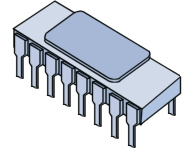
\includegraphics[height=2cm]{../illustration/circuit_integre.png}
\end{figure}
\end{itemize}
\end{frame}


\subsection{Les systèmes de traitement par lots}
%------------------------------------------------------------------- 

\begin{frame}{Les systèmes de traitement par lots}
\begin{definition}
En informatique, un traitement par lots (\emph{batch processing}) est
un enchaînement automatique de commandes sans intervention d'un opérateur.
\end{definition}
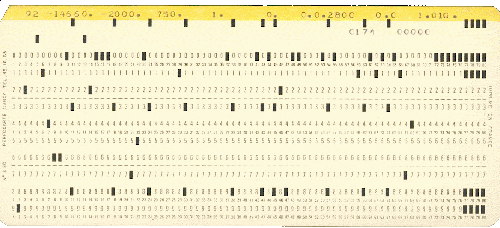
\includegraphics[height=2cm]{../illustration/carte_jcl.png}
\end{frame}


\begin{frame}{Les systèmes de traitement par lots}
\begin{columns}
\column{.5\textwidth}
\begin{block}{Progrès du matériel}
\begin{itemize}
\item Mémoires
\item Transistors, puis circuits intégrés
\item Périphériques
\begin{itemize}
\item lecteurs/perforateurs de cartes et de rubans
\item imprimantes
\item tambours
\item bandes magnétiques
\end{itemize}
\end{itemize}
\end{block}
\column{.5\textwidth}
\begin{block}{Progrès du logiciel}
\begin{itemize}
\item Assembleur
\item Langages évolués :
\begin{itemize}
\item FORTRAN (1957)
\item ALGOL (1960)…
\end{itemize}
\item Moniteur d’enchaînement résident
\end{itemize}
\end{block}
\end{columns}
\end{frame}

\begin{frame}{Les systèmes de traitement par lots}
\begin{itemize}
\item Système d'exploitation simple 
\begin{itemize}
\item Moniteur d’enchaînement résident
\item OS/360 d’IBM
\end{itemize}
\item Pas d'interaction directe utilisateur/système
\begin{itemize}
\item Entrée : Lecteurs de carte/bande
\item Sortie : Perforateurs, bandes, imprimantes
\end{itemize}
\item Regroupement des tâches en lots
\begin{itemize}
\item Suite de cartes
\item Exécution différée
\end{itemize}
\end{itemize}
\end{frame}

\begin{frame}{Moniteur d’enchaînement (1955)}
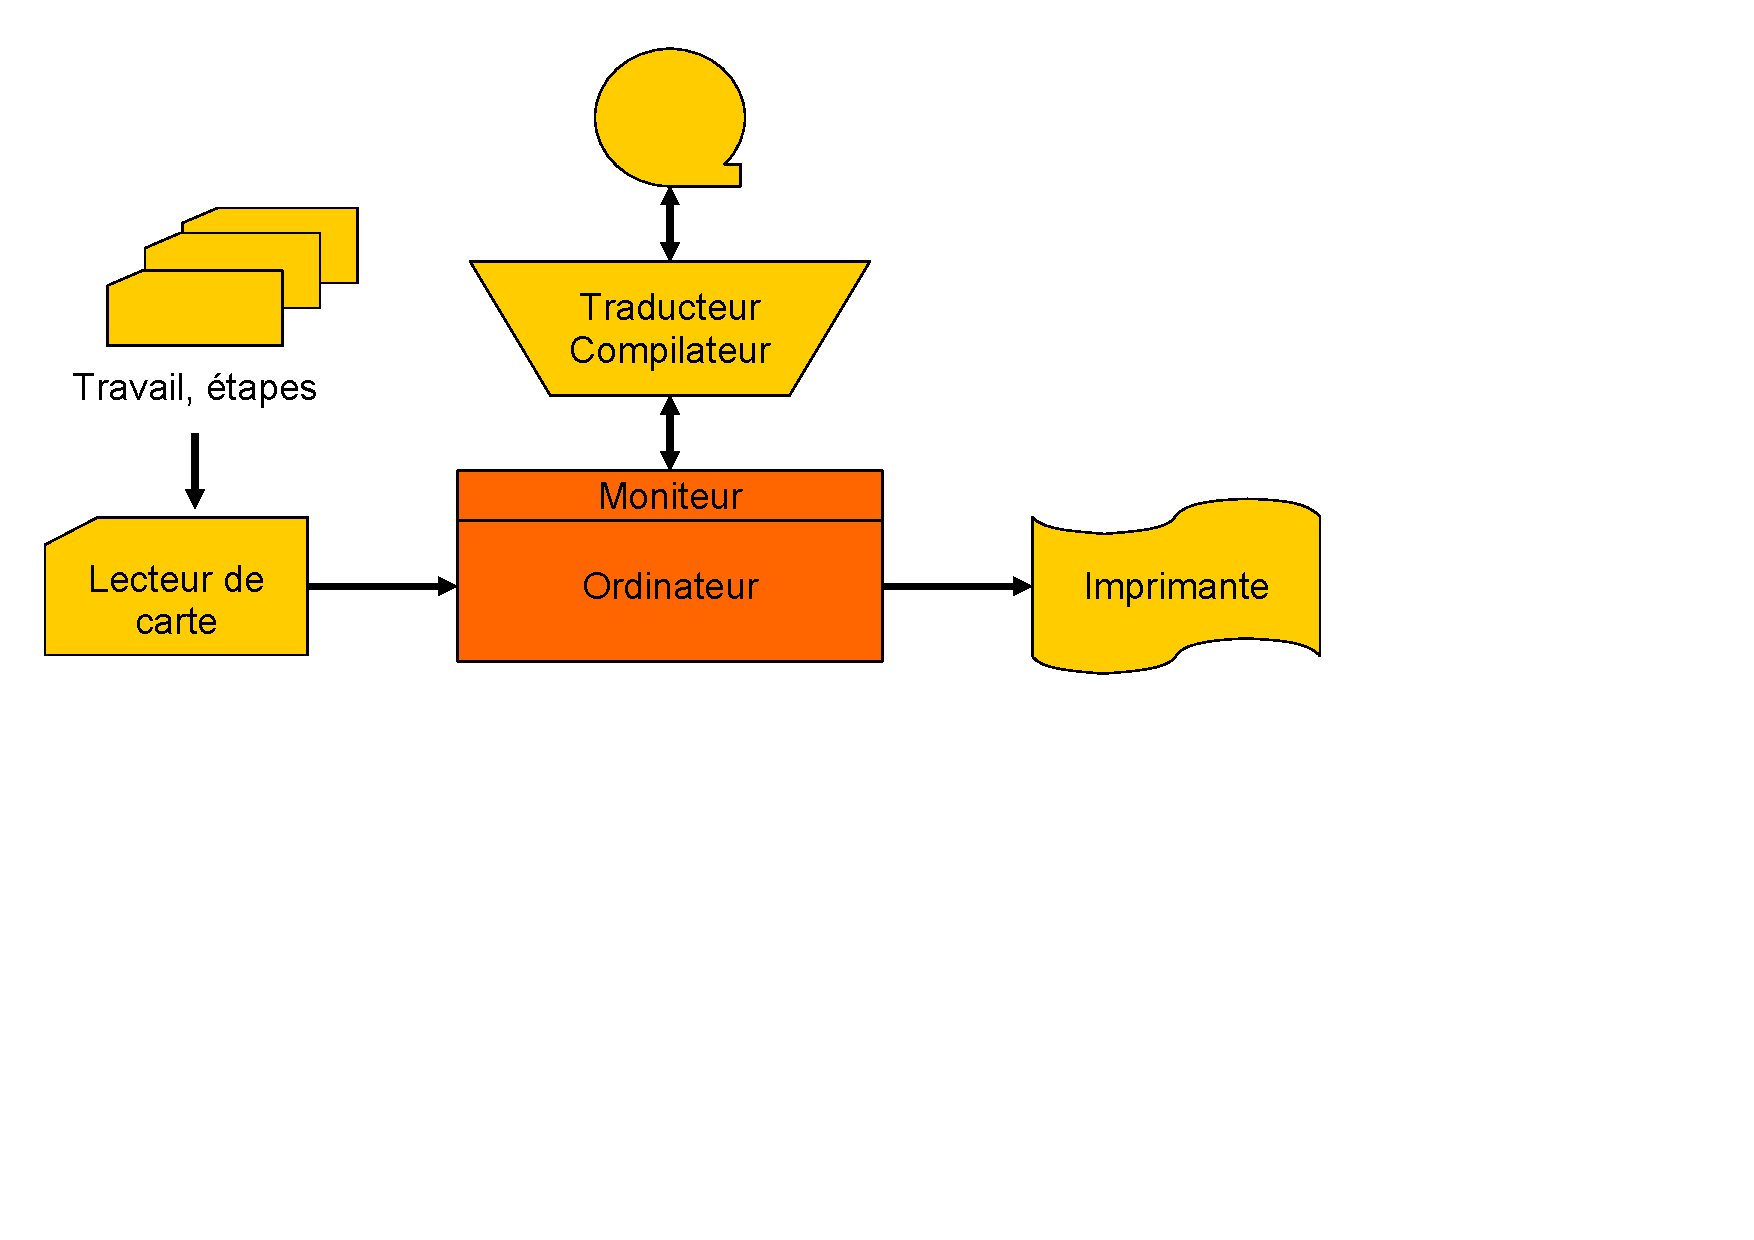
\includegraphics[height=5cm]{../illustration/moniteur_enchainement.pdf}
\end{frame}

\begin{frame}{Session de travail typique (JCL)}
\begin{itemize}
\item Cartes de contrôle : renseignements sur les travaux
\item Carte de début de travail (\$JOB)
\item Carte de début de compilation (\$LOAD)
\item Cartes du source
\item Carte de fin de compilation
\item Carte de début d’exécution (\$RUN)
\item Cartes de données
\item Carte de fin d’exécution
\item Carte de fin de travail
\end{itemize}
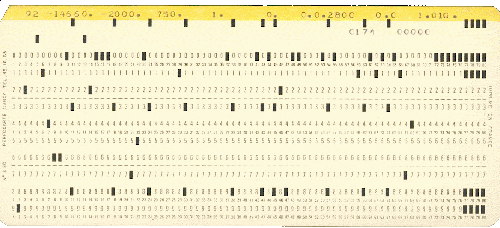
\includegraphics[height=1cm]{../illustration/carte_jcl.png}
\end{frame}

\begin{frame}{La problématique de l'attente des E/S}
Perte de cycles CPU
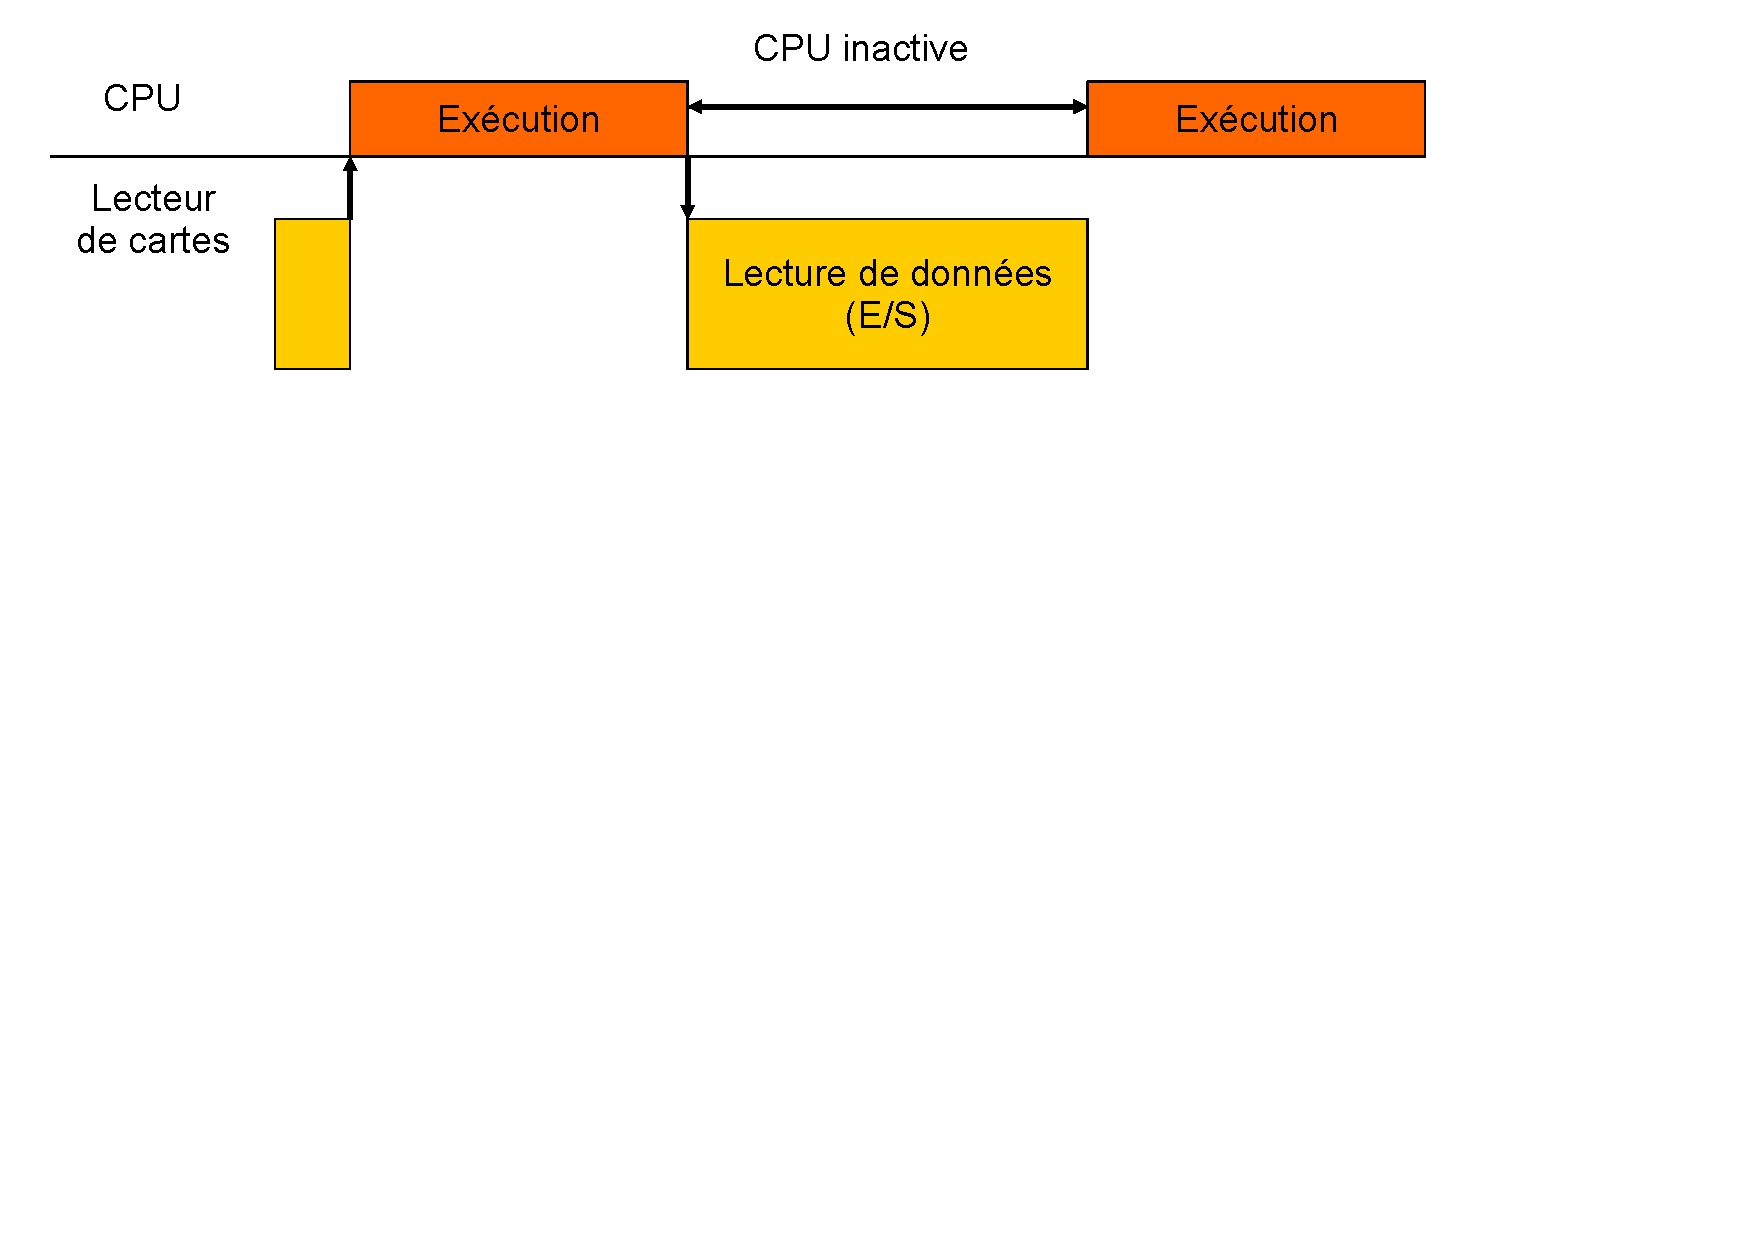
\includegraphics[width=11cm]{../illustration/attente_es.pdf}
\end{frame}

\begin{frame}{Ordinateur auxiliaire (1960)}
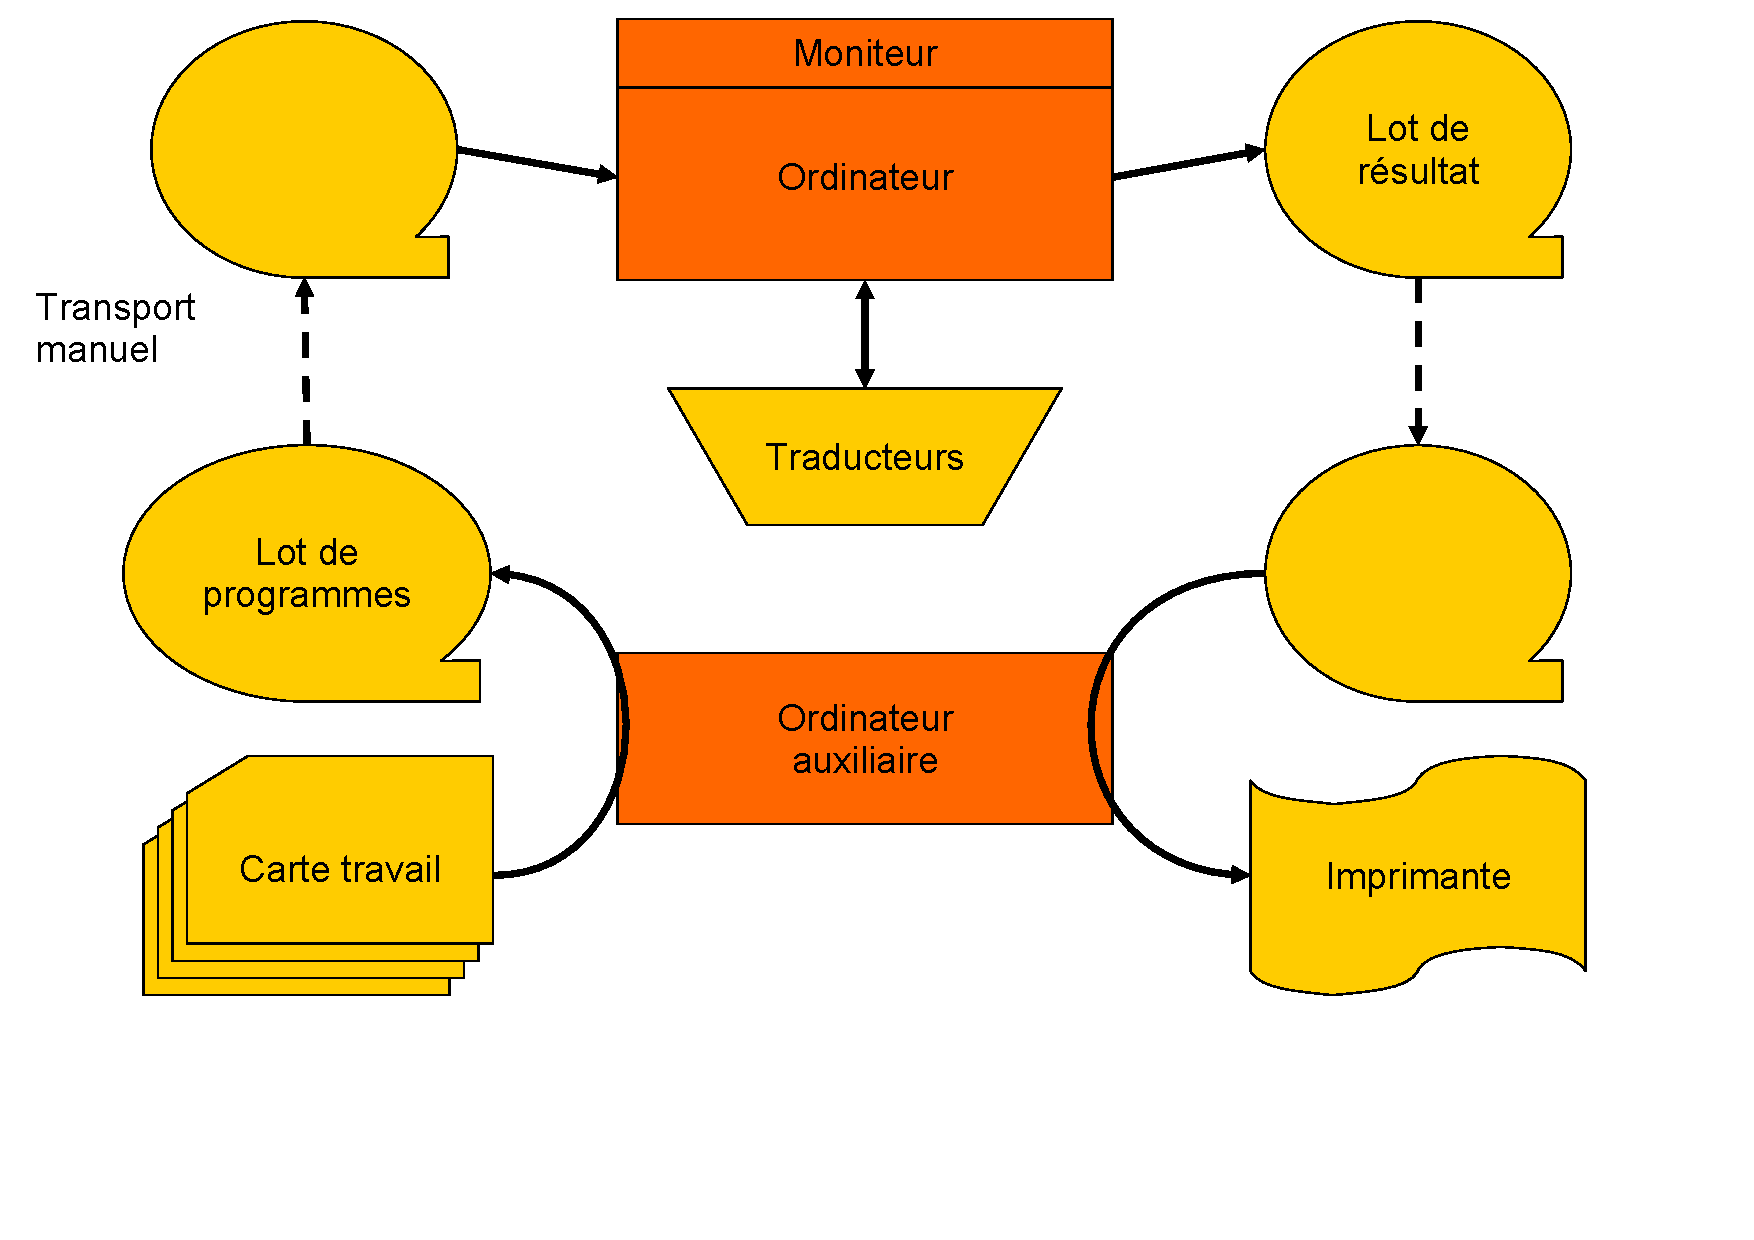
\includegraphics[height=5cm]{../illustration/ordinateur_aux.pdf}
\end{frame}

\begin{frame}{Les systèmes de traitement par lot}
\begin{columns}
\column{.5\textwidth}
\begin{block}{Avantages}
\begin{itemize}
\item Utilisation de langages de commande évolués
\item Préparation des travaux indépendante de l’exploitation
\item Débit amélioré (meilleure utilisation du matériel)
\end{itemize}
\end{block}
\column{.5\textwidth}\begin{block}{Inconvénients}
\begin{itemize}
\item Pas d'interaction directe utilisateur/système
\item Monoprogrammation
\begin{itemize}
\item Processeurs souvent inactif
\end{itemize}
\item Temps de réponse augmenté
\end{itemize}
\end{block}
\end{columns}
\end{frame}

\begin{frame}{Exemple : Univac 1}
\begin{columns}
\column{.5\textwidth}
\begin{itemize}
\item UNIVersal Automate Computer
\item Lancé en 1951
\item 48 exemplaires
\item 4 millions d'Euro
\item 125 kW
\item 48 kO de mémoire
\item 1900 opérations par seconde
\end{itemize}
\column{.5\textwidth}
	\begin{center}
	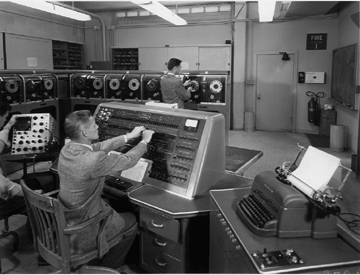
\includegraphics[width=6cm]{../illustration/univac.png}
	\end{center}
\end{columns}
\end{frame}



\subsection{Les systèmes multiprogrammés / à temps partagé}
%------------------------------------------------------------------- 
\begin{frame}{Les systèmes multiprogrammés}
\begin{definition}
Se dit d'un système à multiprogrammation, c'est à dire capable de faire tourner plusieurs programmes en même temps.
\end{definition}
\begin{itemize}
\item Permet d'occuper le processeur pendant les phases d'E/S
\item Taux de multiprogrammation : \begin{itemize}
\item nombre de programmes actifs simultanément
\end{itemize}

\end{itemize}
\end{frame}


\begin{frame}{Evolution technologique}
\begin{columns}
\column{.5\textwidth}
\begin{block}{Progrès du matériel}
\begin{itemize}
\item Amélioration des périphériques
\item Processeurs dédiés aux entrées-sorties
\begin{itemize}
\item E/S tamponnées
\end{itemize}
\item Organisation de la mémoire
\begin{itemize}
\item mémoire virtuelle
\item pagination
\end{itemize}
\end{itemize}
\end{block}
\column{.5\textwidth}
\begin{block}{Progrès du logiciel}
\begin{itemize}
\item Entrées-sorties en mode différé
\begin{itemize}
\item spool
\end{itemize}
\item Exécution parallèle d’entrée-sortie et d’activités d’exécution
\begin{itemize}
\item E/S tamponnée
\end{itemize}
\item Moniteur plus évolué
\end{itemize}
\end{block}
\end{columns}
\end{frame}

\begin{frame}{E/S tamponnées}
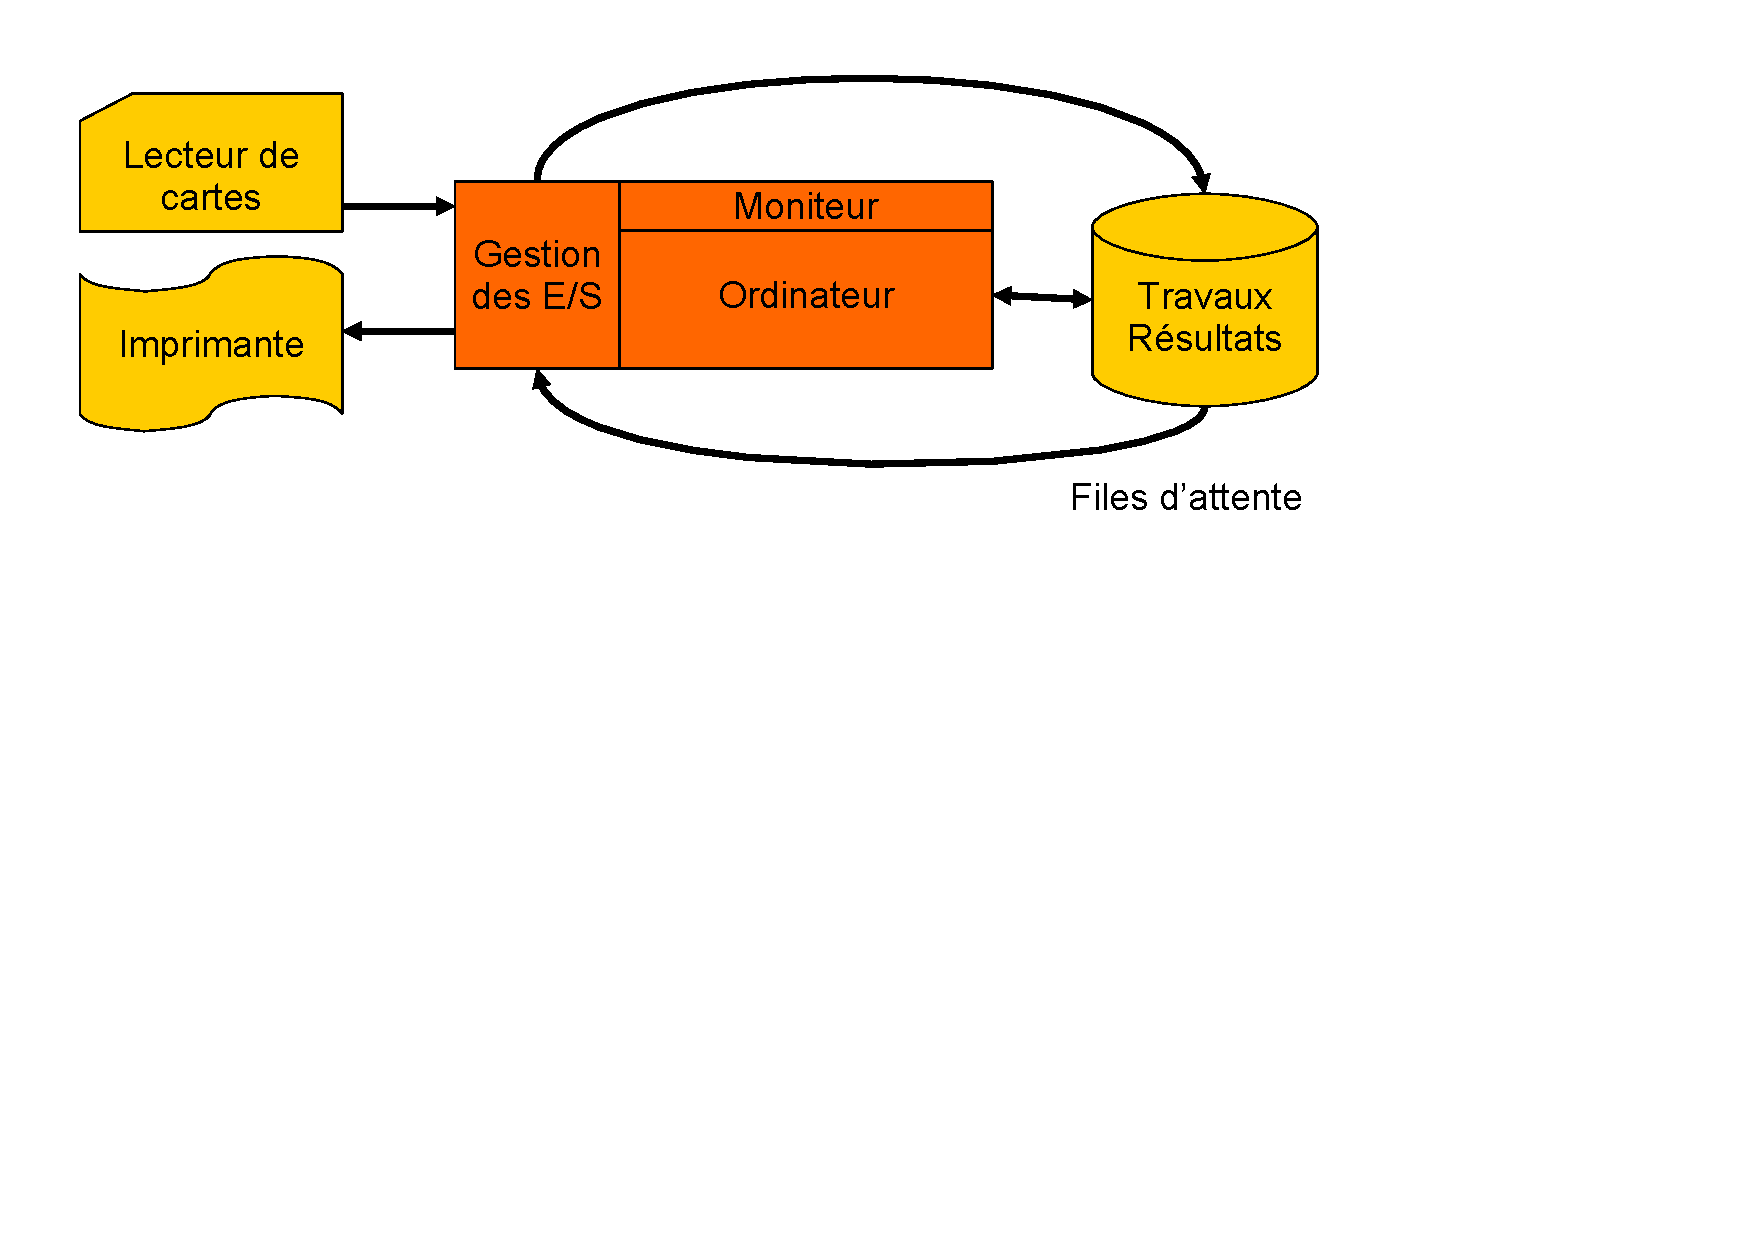
\includegraphics[width=11cm]{../illustration/es_tampon.pdf}
\end{frame}

\begin{frame}{Principes des systèmes multiprogrammés}
\begin{itemize}
\item Plusieurs travaux en mémoire
\item Chaque travail utilise la CPU jusqu’à être interrompu par une E/S
\begin{itemize}
\item Exécution exclusive de chaque travail
\end{itemize}
\item Ordonnancement des travaux par le moniteur
\end{itemize}
\end{frame}

\begin{frame}{E/S tamponnées}
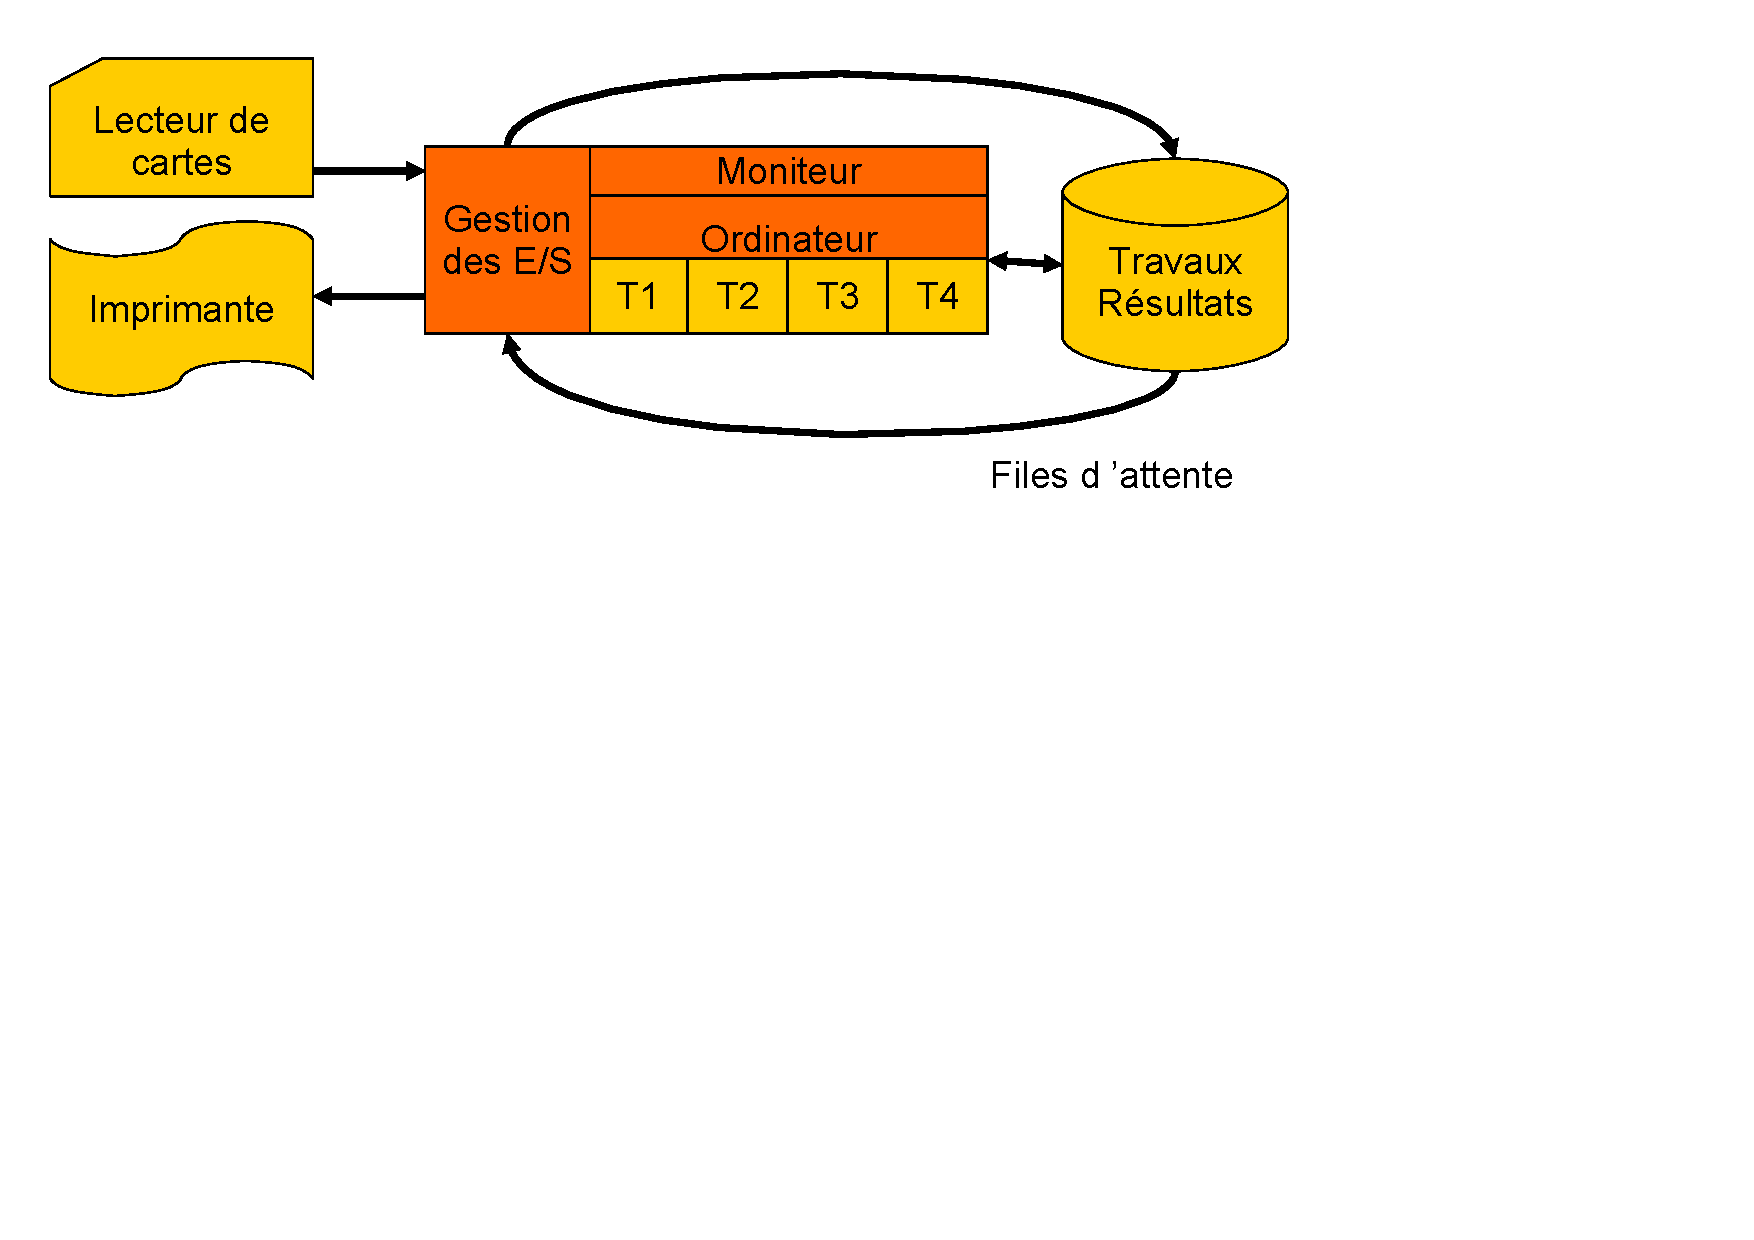
\includegraphics[width=11cm]{../illustration/systeme_multiprogramme.pdf}
\end{frame}

\begin{frame}{Traitement des E/S}
Optimisation de l'utilisation de la CPU
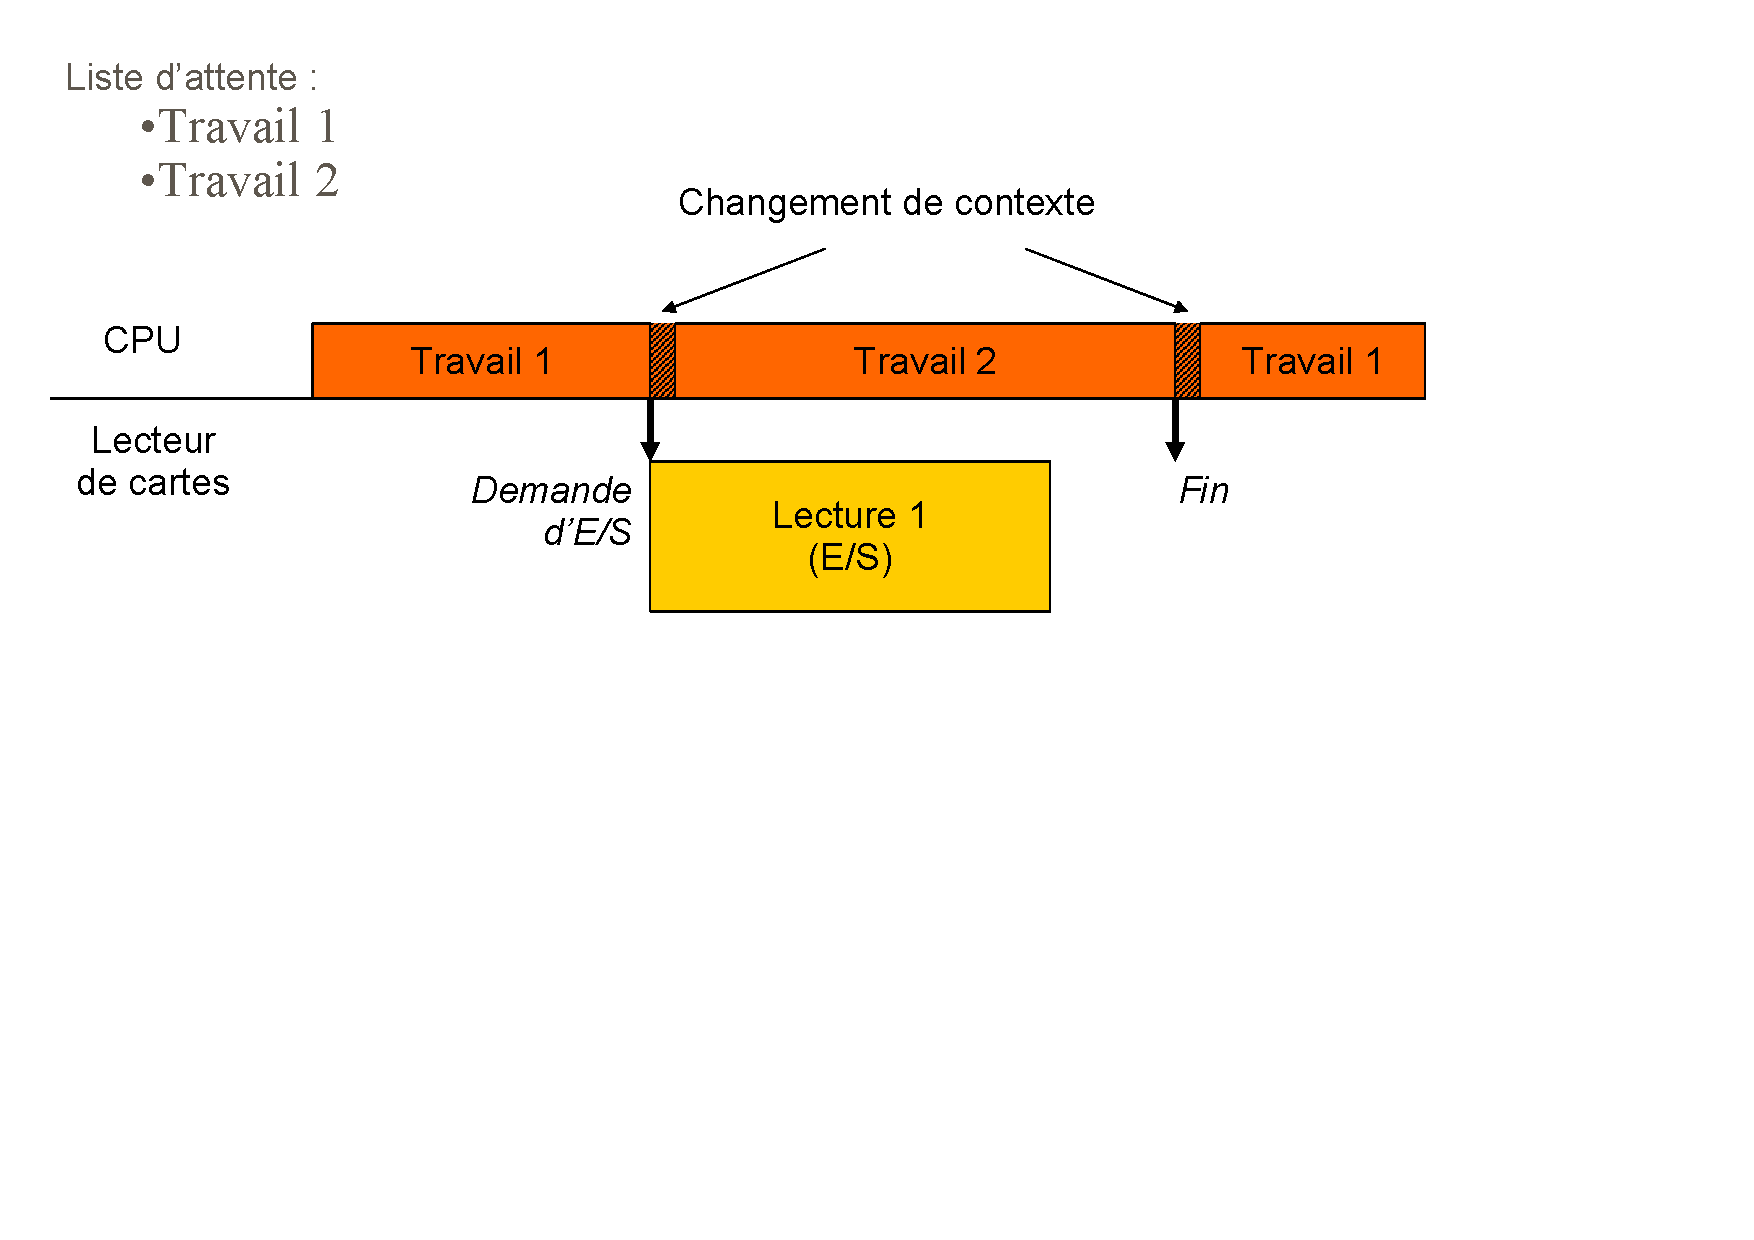
\includegraphics[width=11cm]{../illustration/systeme_multiprogramme_enchainement.pdf}
\end{frame}

\begin{frame}{Les systèmes multiprogrammés}
\begin{columns}
\column{.5\textwidth}
\begin{block}{Avantages}
\begin{itemize}
\item Meilleure utilisation du processeur
\begin{itemize}
\item meilleur débit
\end{itemize}
\item Efficace pour les travaux courts \begin{itemize}\item bon temps de réponse \end{itemize}
\item Protection du moniteur
\begin{itemize}
\item superviseur des entrées/sorties
\end{itemize}
\end{itemize}
\end{block}
\column{.5\textwidth}\begin{block}{Inconvénients}
\begin{itemize}
\item Partage des ressources
\begin{itemize}
\item mémoire centrale
\item CPU
\item E/S...
\item changement de contexte après chaque interruption
\end{itemize}
\item Temps de réponse variables
\item Risque de pénurie
\end{itemize}
\end{block}
\end{columns}
\end{frame}


\begin{frame}{Les systèmes à temps partagé}
\begin{definition}
Technique d’exploitation d’un système informatique qui assure l’imbrication dans le temps 
de plusieurs processus dans un même processeur [AFNOR]
\end{definition}
\end{frame}

\begin{frame}{Les systèmes à temps partagé}
\begin{itemize}
\item Introduit en 1965
\begin{itemize}
\item Extension de la multiprogrammation
\end{itemize}
\item Commutations fréquentes
\begin{itemize}
\item Utilisation d’une horloge
\item Quantum de temps\note{$$x * \frac{1}{100} seconde$$}
\item Interruption des travaux par le système
\end{itemize}
\item Illusion de traitement multi-tâches
\begin{itemize}
\item Interaction avec l'utilisateur
\item Utilisation de terminaux
\end{itemize}
\end{itemize}
\end{frame}

\begin{frame}{Enchaînement de tâche dans un système à temps partagé}
Optimisation des temps de réponse
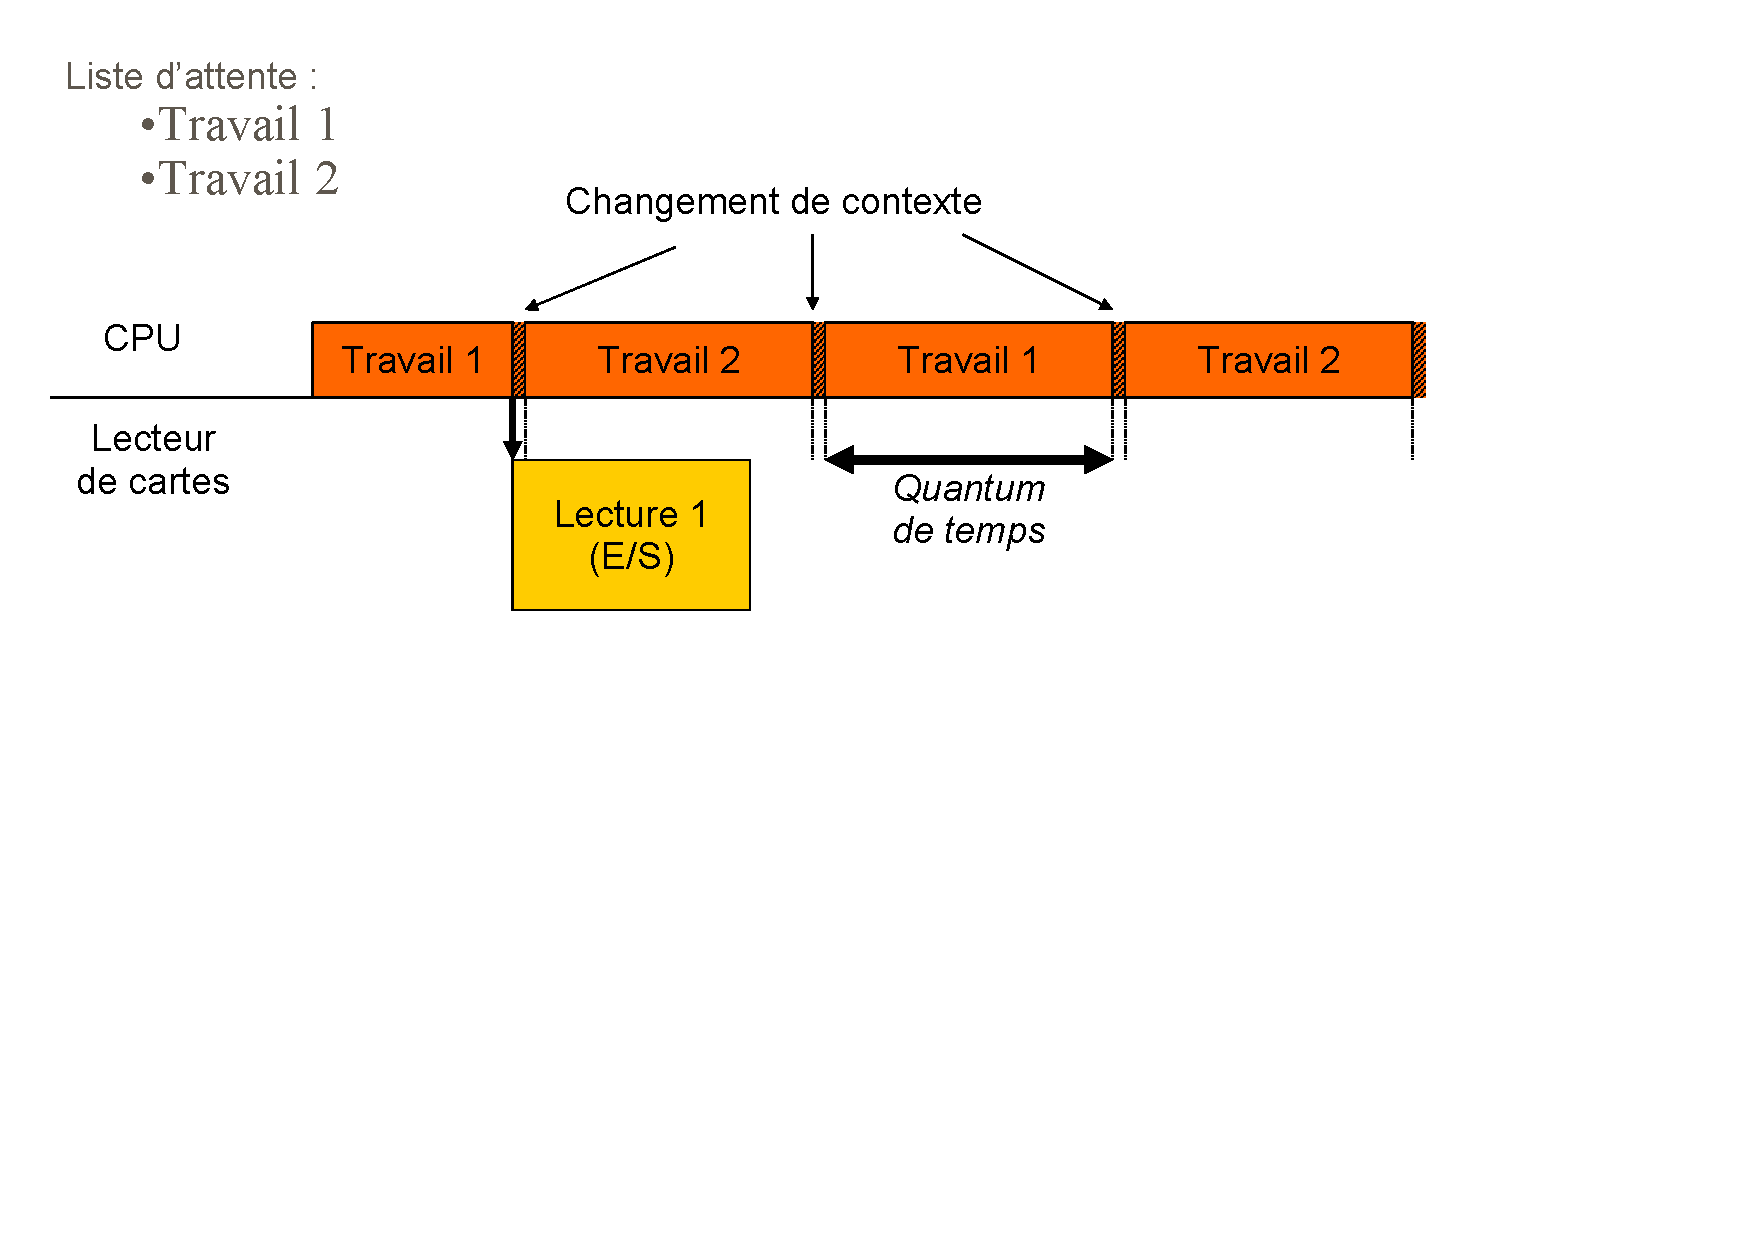
\includegraphics[height=5cm]{../illustration/systeme_tps_partage_enchainement.pdf}
\end{frame}

\begin{frame}{Les systèmes à temps partagé}
\begin{columns}
\column{.5\textwidth}
\begin{block}{Avantages}
\begin{itemize}
\item Meilleur temps de réponse
\begin{itemize}
\item délai d’attente plus court
\end{itemize}
\item Interaction utilisateur
\item Illusion multi-tâches
\end{itemize}
\end{block}
\column{.5\textwidth}\begin{block}{Inconvénients}
\begin{itemize}
\item Complexité
\item Pas réellement multi-tâches
\item Perte d'efficacité
\begin{itemize}
\item changements de contexte fréquents
\end{itemize}
\end{itemize}
\end{block}
\end{columns}
\end{frame}


\begin{frame}{Le micro-processeur}
\begin{itemize}
\item Intégration de tous les éléments d'un processeur dans un unique circuit intégré
\item Premier microprocesseur : 
\begin{itemize}
\item Intel 4004 en 1971
\item unité de calcul de 4 bits, cadencé à 108 kHz
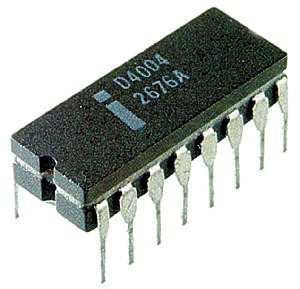
\includegraphics[height=3cm]{../illustration/Intel4004.jpg}
\end{itemize}
\item Très complexe à mettre au point, bon marché (200 dollars)
\end{itemize}
\end{frame}

\begin{frame}{Loi de Moore (1965)}
Basée sur des observations empiriques
\begin{itemize}
\item Doublement du nombre de transistors intégrés dans une puce tous les 18 mois
\item Vérifiée pendant 30 ans
\item Bornée aux limites physiques
\begin{itemize}
\item pratiquement atteintes aujourd'hui
\item problématiques de l'enveloppe thermique et de l'efficacité énergétique
\item nécessite de nouvelles techniques de gravure (finesse extrême, circuits 3D\footnote{FinFet 14nm, chez AMD, par exemple.}... )
\end{itemize}
\end{itemize}
\end{frame}


\begin{frame}{Loi de Moore (1965)}
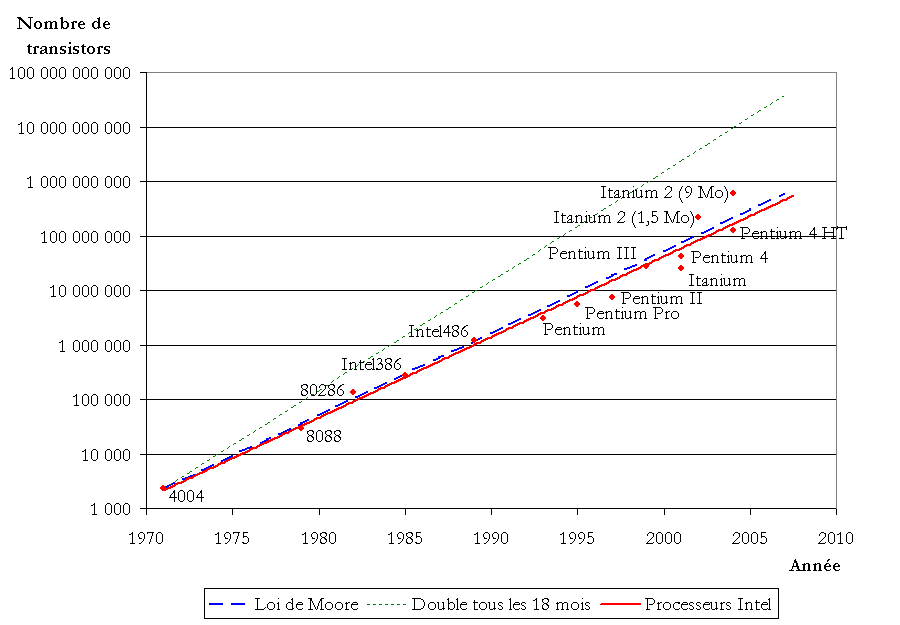
\includegraphics[height=6.5cm]{../illustration/Evolutionprocesseurs.png}
\end{frame}


\subsection{Les systèmes parallèles / distribués}
%------------------------------------------------------------------- 
\begin{frame}{Les systèmes parallèles}
\begin{itemize} 
\item Utilisation de plusieurs processeurs
\begin{itemize}
\item processeurs courants
\item moins coûteux que les processeurs spécifiques
\item mémoire partagée ou répartie
\item même bus de données
\end{itemize}
\item Utilisation de processeurs multi-cœurs (multicores)
\begin{itemize}
\item intégrés dans un seul circuit
\item tendance récente en cours de généralisation
\item performances liées à la topologie d'interconnexion des cœurs
\end{itemize}
\item Partage des travaux - exécution simultanée
\end{itemize}
\end{frame}

\begin{frame}{Deux familles de systèmes parallèles}
\begin{columns}
\column{.5\textwidth}
\begin{block}{Symétriques (SMP)}
\begin{itemize}
\item Plusieurs processeurs égaux
\item Les processeurs exécutent tous une copie du système
\item Partage collaboratif des travaux
\end{itemize}
\end{block}
\column{.5\textwidth}
\begin{block}{Asymétriques (AMP)}
\begin{itemize}
\item Un processeur pilote
\item Attribue les travaux aux autres
\item Possibilité spécialisation de processeurs
\end{itemize}
\end{block}
\end{columns}
\end{frame}

\begin{frame}{Systèmes parallèles}
\begin{columns}
\column{.5\textwidth}
\begin{block}{Avantages}
\begin{itemize}
\item Scalabilité
\begin{itemize}
\item Possibilité d'augmenter la puissance au besoin
\end{itemize}
\item Efficacité
\begin{itemize}
\item Coût raisonnable
\item Réellement multi-tâches
\end{itemize}
\item Fiabilité
\begin{itemize}
\item Tolérances aux pannes (dans le cas du SMP)
\end{itemize}
\end{itemize}
\end{block}
\column{.5\textwidth}
\begin{block}{Inconvénients}
\begin{itemize}
\item Équilibrage de charge entre les processeurs
\begin{itemize}\item Difficulté de gestion des files d'attente\end{itemize}
\item Concurrence d'accès aux ressources
\item Manque de souplesse
\end{itemize}
\end{block}
\end{columns}
\end{frame}


\begin{frame}{Machine à bus unique - Mémoire centralisée}
Machine à bus unique Mémoire centralisée
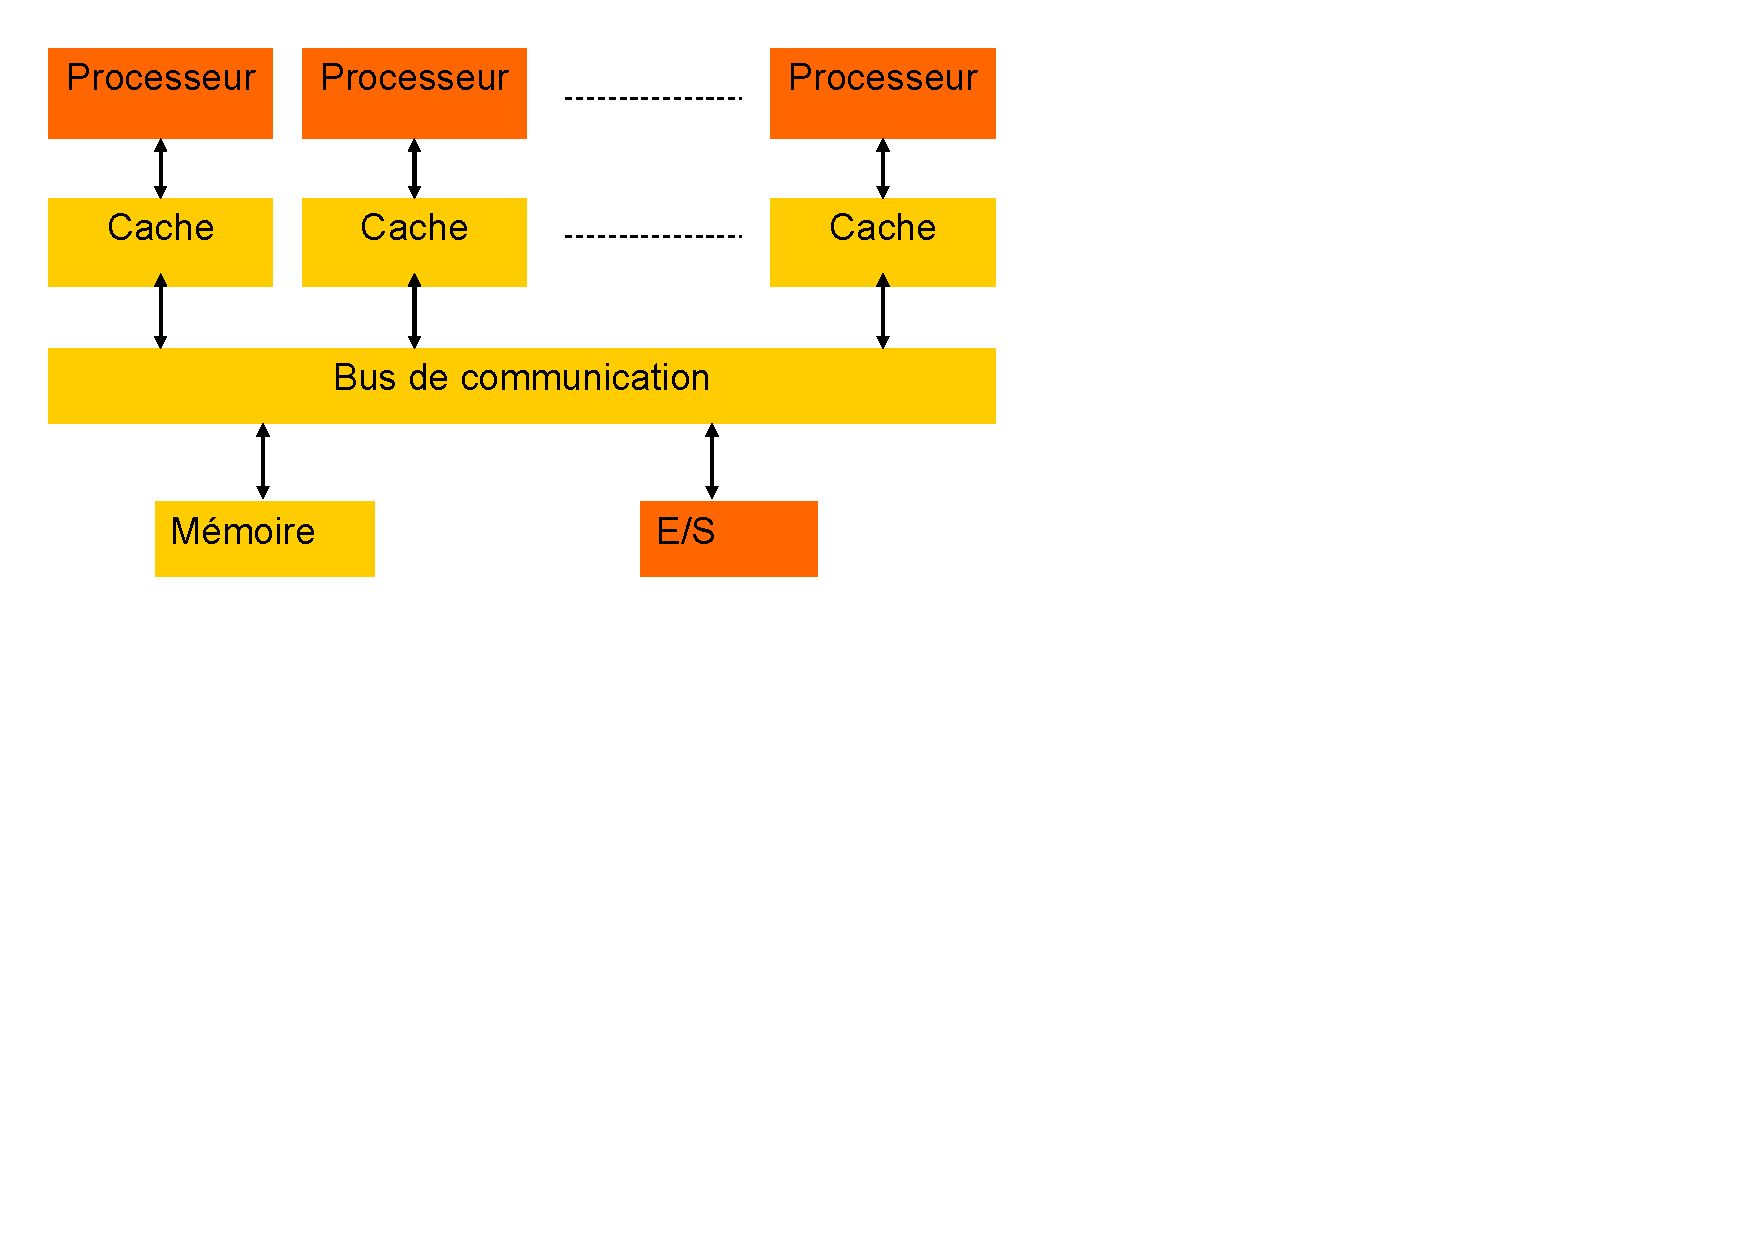
\includegraphics[height=5cm]{../illustration/para_mem_commun.pdf}
\end{frame}

\begin{frame}{Mémoire distribuée}
Machine à bus unique Mémoire distribuée (NUMA)
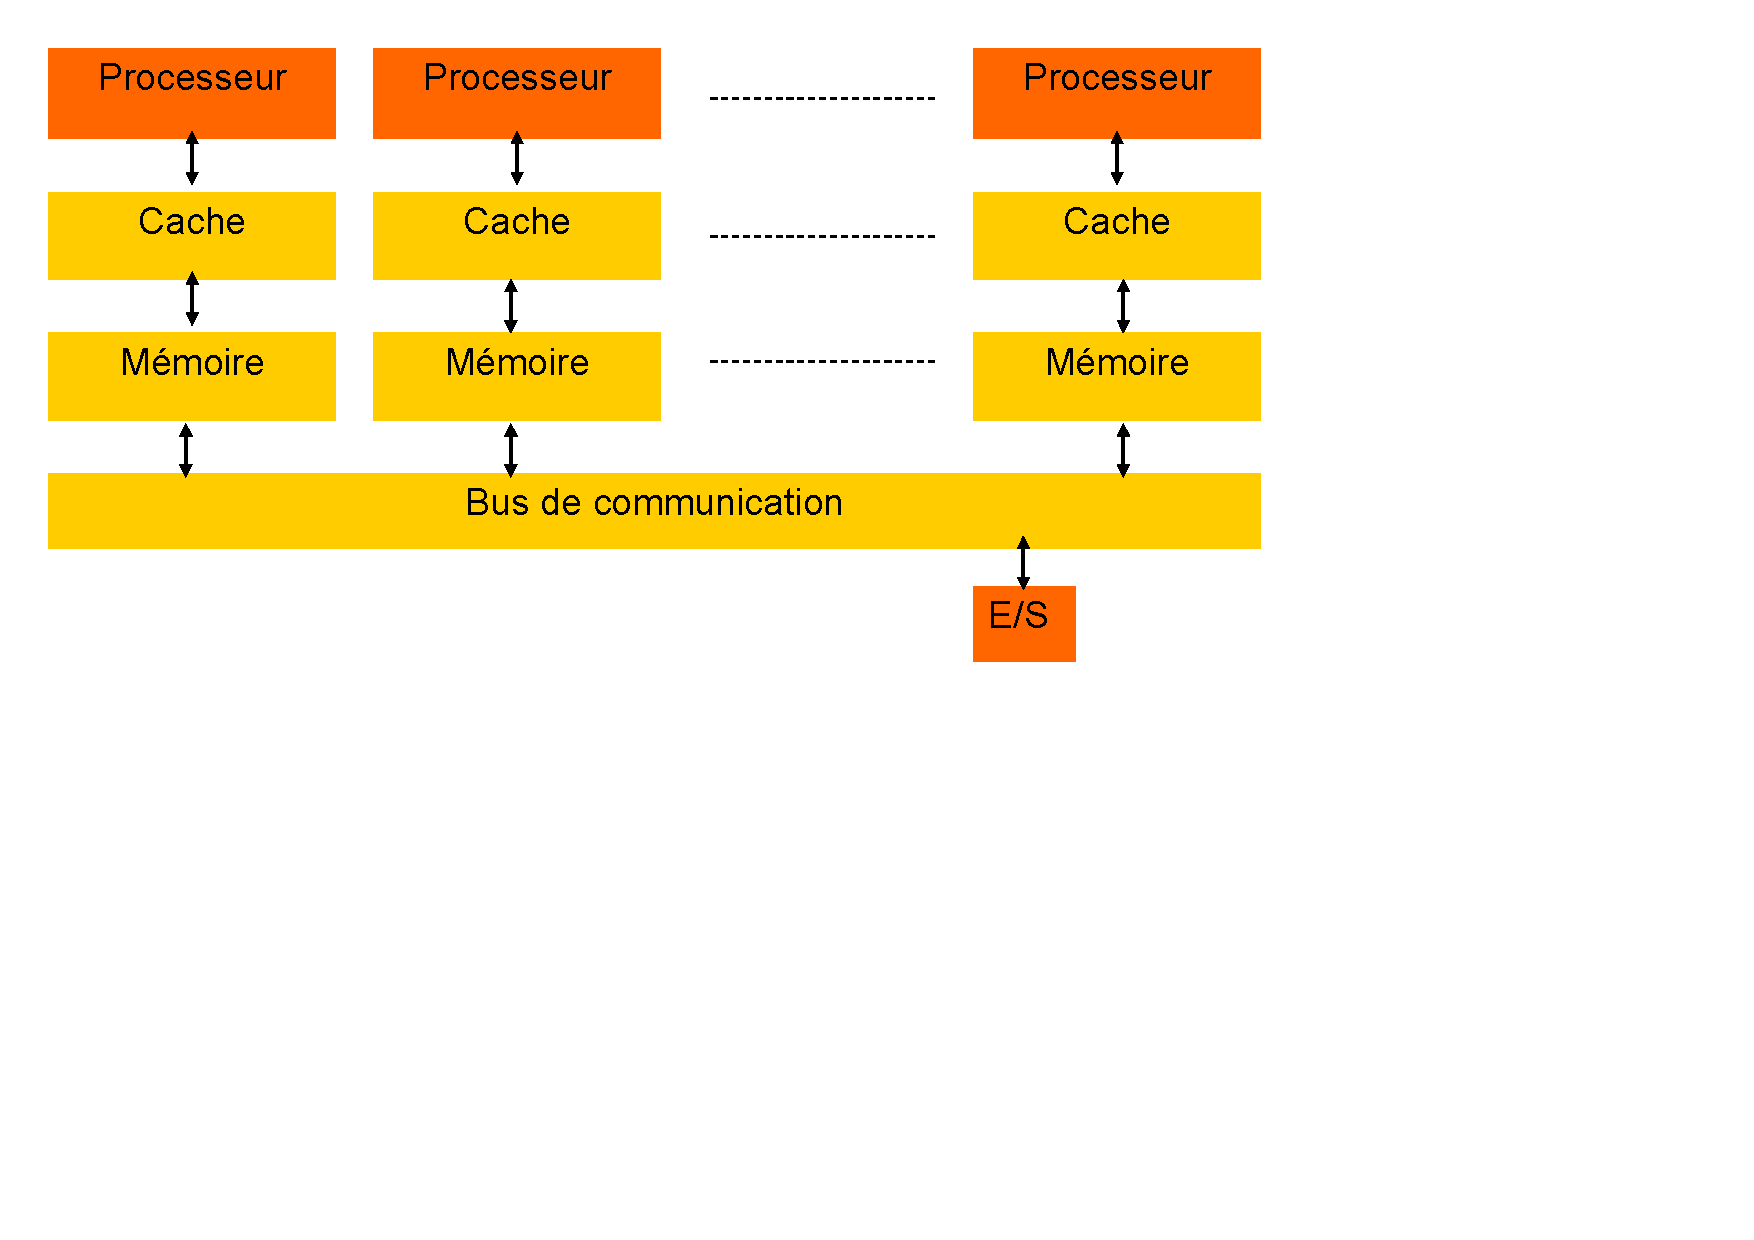
\includegraphics[height=5cm]{../illustration/para_mem_distri.pdf}
\end{frame}

\begin{frame}{Taxinomie de Flynn \cite{wp-flynn}}
Classification architectures d'ordinateur - Michael J. Flynn (1966)
\begin{itemize}
\item <1->[SISD] Ordinateur séquentiel, aucun parallélisme
\item <2->[SIMD] Parallélisme au niveau de la mémoire (processeur vectoriel)
\item <3->[MISD] Même donnée traitée par plusieurs processeurs en parallèle. Usage spécialisé (filtrage numérique, vérification de redondance dans les systèmes critiques...)
\item <4->[MIMD] Ordinateur parallèle : plusieurs processeurs traitent des données distinctes
\begin{itemize}
\item MIMD à mémoire partagée. Espace d'adressage global. Communication inter-CPU via la mémoire globale.
\item MIMD à mémoire distribuée. Chaque CPU a sa propre mémoire et son propre système d'exploitation.

Middleware pour la synchronisation et la communication. 
\end{itemize}
\end{itemize}
\end{frame}


\begin{frame}{Les systèmes distribués}
\begin{itemize}
\item Tous les processeurs ne partagent pas le même bus de données et la même mémoire
\begin{itemize}
\item Communication via un réseau
\end{itemize}
\item Partage de ressources sur un réseau
\begin{itemize}
\item Grappe de calcul
\item Cluster
\end{itemize}
\item Plusieurs ordinateurs qui collaborent
\begin{itemize}
\item Mêmes mécanismes que pour les systèmes parallèles
\item Problématique des délais de propagation des informations
\end{itemize}
\end{itemize}
\end{frame}

\begin{frame}{Les systèmes distribués}
\begin{columns}
\column{.5\textwidth}
\begin{block}{Avantages}
\begin{itemize}
\item Réellement multi-tâches
\item Tolérance aux pannes
\item Souplesse, évolutivité
\end{itemize}
\end{block}
\column{.5\textwidth}
\begin{block}{Inconvénients}
\begin{itemize}
\item Délais de propagation
\item Équilibrage de charge entre les ordinateurs connectés
\item Complexité
\begin{itemize}
\item Administration
\item Optimisation
\end{itemize}
\end{itemize}
\end{block}
\end{columns}
\end{frame}

\begin{frame}{Clusters scientifiques : HPC}
\begin{itemize}
\item \textit{High-Performance Computing}
\item <2->x 1000 tous les 11 ans :
\begin{itemize}
\item 1964 $\rightarrow$ mégaFLOPS : Control Data 6600
\item 1985 $\rightarrow$ gigaFLOPS : Cray-2
\item 1997 $\rightarrow$ téraFLOPS : ASCI Red
\item 2008 $\rightarrow$ pétaFLOPS : Roadrunner
\item ...éxaFLOPS pour les supercalculateurs de 2020 ?
\end{itemize}
\item <3->Record actuel\footnote{2015} : 
\begin{itemize}
\item Réseau de minage Bitcoin = 3 750 éxaFLOPS
\item Tianhe 2 (défense chinoise) : 32 000 Xeon Ivy Bridge + 48 000 Xeon Phi = 33,86 petaflops
\end{itemize}

\item <4->Un PC de 2013 :
\begin{itemize}
\item CPU Intel Core i7-3770 $\rightarrow$ 200 gigaFLOPS
\item GPU NVidia GTX 690 $\rightarrow$ 5 621 gigaFLOPS (record de 2001)
\end{itemize}
\end{itemize}
\end{frame}

\begin{frame}{Botnet \cite{wp-botnet} : réseau de bots informatiques}
\begin{itemize}
\item Bot : \begin{itemize}
\item Agent logiciel (semi)automatique connecté à Internet
\item Communique avec d'autres programmes similaires
\begin{itemize}
\item robots IRC, machines zombies...
\end{itemize}
\item Effectuent des tâches bien identifiées
\begin{itemize}
\item spam, DoS, cassage de clefs de cryptage...
\end{itemize}
\end{itemize}

\item Grosse capacité de traitement :
\begin{itemize}
\item Entre 4 000 et 5 000 botnets actifs février 2012
\item 13 million de machines pour le plus gros botnet identifié\footnote{En 2013}
\end{itemize}
\item Location à l'usage
\begin{itemize}
\item Verisign 2010 (iDefense Intelligence Operations Team)
\item 9\$ l'heure ou 67\$ les 24h, en moyenne 
\end{itemize}

\end{itemize}
\end{frame}

\begin{frame}{IaaS : Infrastructure as a service \cite{wp-IaaS}}
Infrastructure as a service (IaaS) :
\begin{itemize}
\item ressources informatiques (CPU, stockage, réseau... )
\item capacité de traitement
\item ressources de stockage...
\end{itemize}

Fondement du Cloud Computing\cite{wp-cloud} pour les infrastructures :
\begin{itemize}
\item \underline{Ressources} en self-service, adaptation à la demande
\item \underline{Ouverture}, via interfaces standardisées
\item \underline{Mutualisation} et présentation des ressources sous la forme d'un système virtuel unique (grilles informatiques)
\item \underline{Paiement à l'usage} : mesure et facturation des ressources consommées
\end{itemize}
\end{frame}

\begin{frame}{IaaS : Infrastructure as a service}
\begin{exampleblock}{Exemples}
\begin{itemize}
\item Amazon EC2 (Elastic Compute Cloud)
\begin{itemize}
\item lancé en 2006, encore largement leader du marché
\item plusieurs dizaines de milliers de serveurs répartis dans le monde
\item 0,45 dollar par heure de traitement (4 vCPU, 15 Go RAM et 1,77 To stockage)
\end{itemize}

\item Google Cloud Compute Engine
\begin{itemize}
\item Lancé en juin 2012
\end{itemize}

\item Microsoft Windows Azure
\begin{itemize}
\item Lancé en juin 2012
\end{itemize}

\item Numergy : \begin{itemize}
\item Cloud français\footnote{Caisse des Dépôts, Bull et SFR} basé sur OpenStack (open source)
\end{itemize}

\end{itemize}
\end{exampleblock}
\end{frame}


\subsection{Les systèmes temps réel}
%------------------------------------------------------------------- 
\begin{frame}{Les systèmes temps réel}
\begin{definition}
Un système temps réel se compose d'un système ou d'une application
devant répondre en un temps fini et spécifié à des stimulis générés
par le monde extérieur
\end{definition}
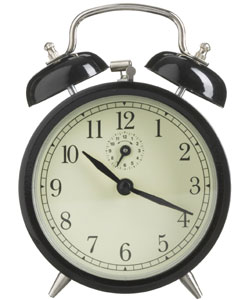
\includegraphics[height=2cm]{../illustration/reveil-ikea.jpg}

\includegraphics[height=2cm]{../illustration/lapin-alice-merveilles.png}
\end{frame}

\begin{frame}
\frametitle{Les systèmes temps réel}
\begin{itemize}
\item Prise en compte de contraintes de temps
\begin{itemize}
\item déterministe
\item temps de réponse garantis
\end{itemize}
\item Deux familles
\begin{itemize}
\item système temps réel \emph{souple}
\item système temps réel \emph{rigide}
\end{itemize}
\end{itemize}
\begin{exampleblock}{Exemples}
\begin{itemize}
\item Souple : multimédia
\item Rigide : contrôle de robots industriels
\end{itemize}
\end{exampleblock}
\end{frame}

\begin{frame}
\frametitle{Types de tâches gérées}
\begin{itemize}
\item Tâches temps réel critiques :
\begin{itemize}
\item Respect absolu des échéances prévues
\end{itemize}
\item Tâches temps réel non-critiques :
\begin{itemize}
\item Peuvent répondre avec un certain retard sachant que la cohérence
      du système en sera dégradée
\end{itemize}
\item Tâches sans contraintes temps réel :
\begin{itemize}
\item Répondre au mieux
\item Doit pouvoir être interrompu à tout moment
\end{itemize}
\end{itemize}
\end{frame}


\subsection{Evaluation des performances}

\begin{frame}
\frametitle{Modes de fonctionnement}
On distingue :
\begin{itemize}
\item Mode différé
\item Mode interactif
\begin{itemize}
\item Transactionnel
\item Machine à usage exclusif
\item Temps partagé
\end{itemize}
\item Mode temps réel
\end{itemize}
\end{frame}

\begin{frame}
\frametitle{Temps de traitement, de rotation}
\begin{itemize}
\item Durée totale de traitement d'un travail
\item Temps entre prise en charge d'un travail et réception de la totalité des résultats
\end{itemize}
\begin{block}{Importance relative}
\begin{tabular}{c|c}
Différé & Long, souvent borné \\
Interactif & Bref, imprévisible (sauf en transactionnel) \\
Temps réel & Très bref, connu \\
\end{tabular}
\end{block}
\end{frame}

\begin{frame}
\frametitle{Délai d’attente (temps de latence)}
\begin{itemize}
\item Délai entre l’envoi d’une commande et le début de l’exécution
\end{itemize}
\begin{block}{Importance relative}
\begin{tabular}{c|c}
Différé & Non représentatif \\
Interactif & Important pour l’interactivité \\
Temps réel & Très bref, $1^{er}$ critère de jugement \\
\end{tabular}
\end{block}
\end{frame}

\begin{frame}
\frametitle{Temps de réponse}
\begin{itemize}
\item Délai entre l’envoi d’une commande et le début de la réponse
\end{itemize}
\begin{block}{Importance relative}
\begin{tabular}{c|c}
Différé & Non représentatif \\
Interactif & 1er critère de jugement \\
Temps réel & Connu, imposé \\
\end{tabular}
\end{block}
\end{frame}


\begin{frame}
\frametitle{Les critères d'évaluation des performances d'un système informatique}
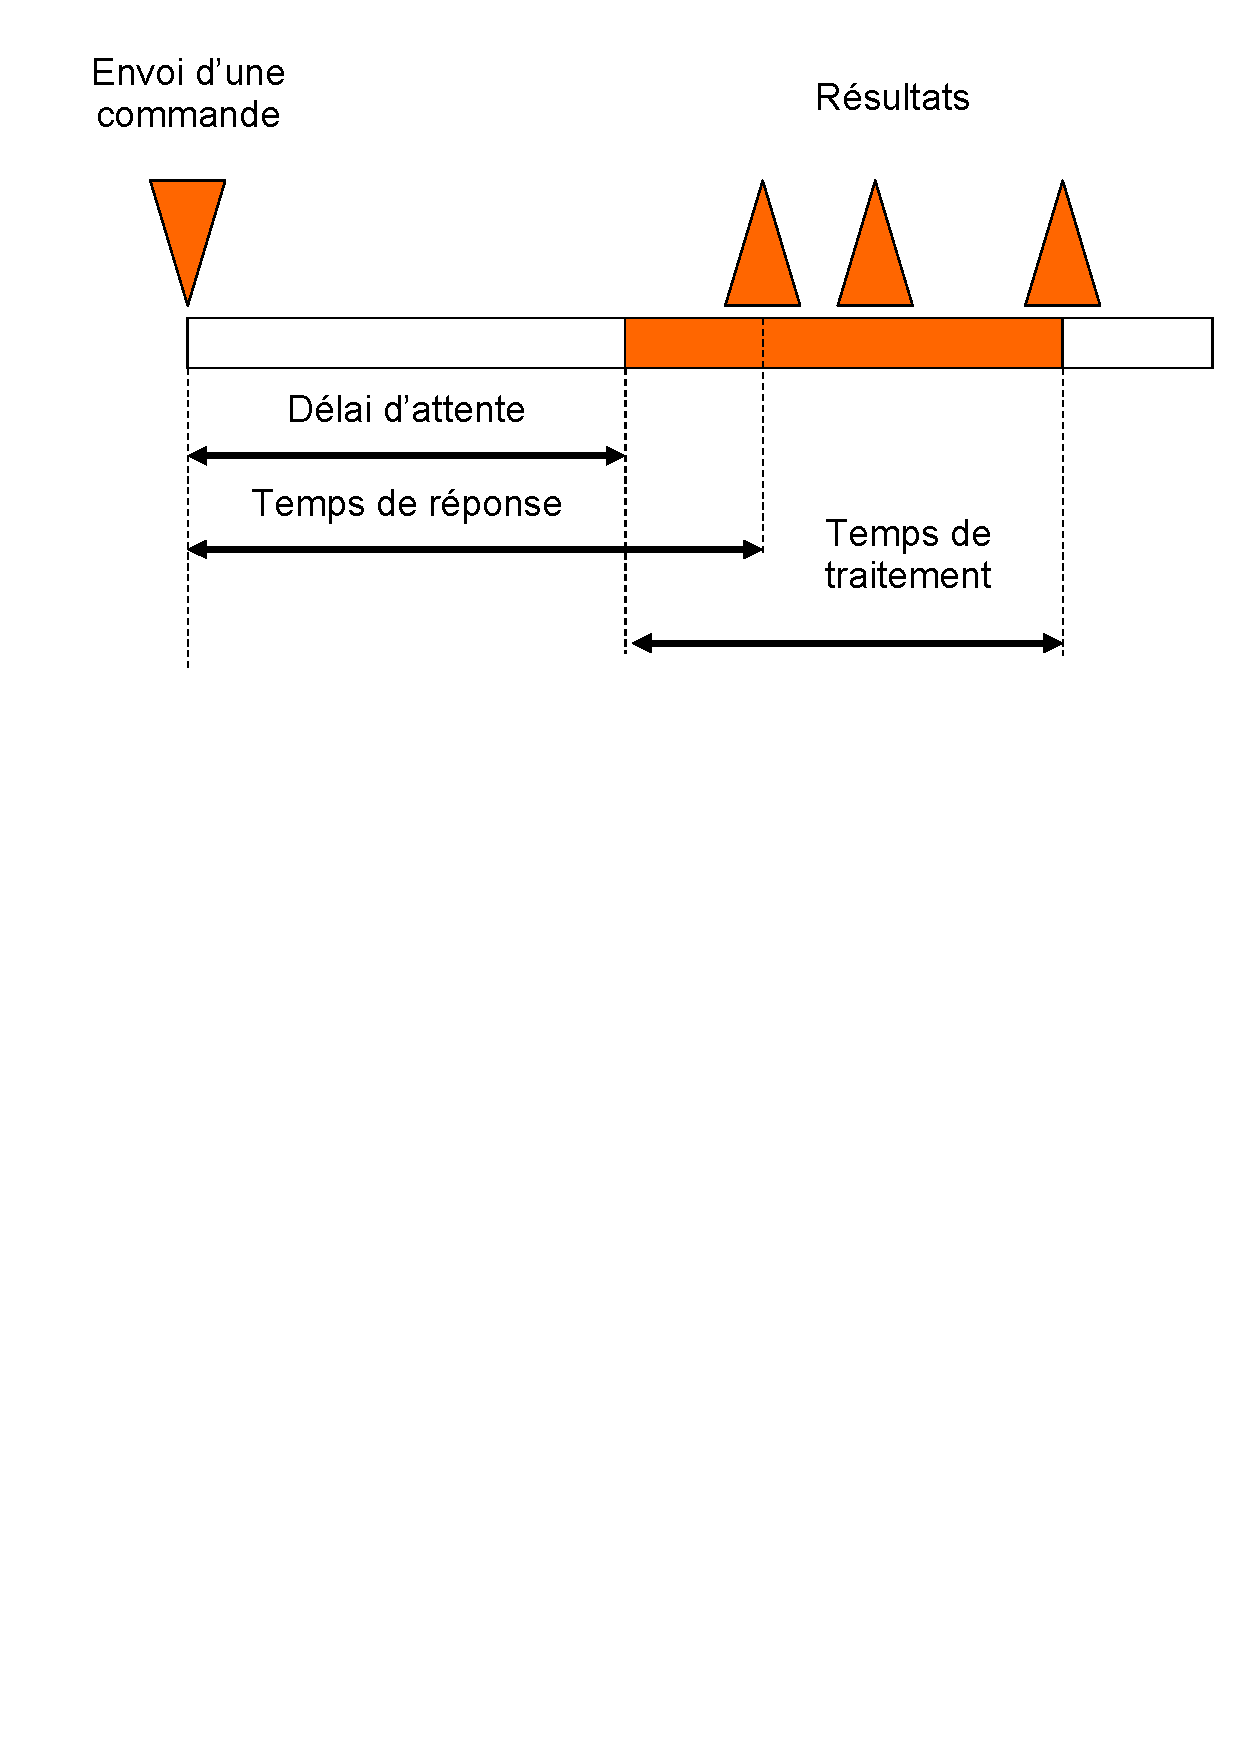
\includegraphics[height=5cm]{../illustration/criteres.pdf}
\end{frame}

\begin{frame}
\frametitle{Débit}
\begin{itemize}
\item Nombre de commandes exécutées par unité de temps
\item Mesure l'efficacité et la rentabilité du système
\end{itemize}
\begin{block}{Importance relative}
\begin{tabular}{c|c}
Différé & Critère de jugement \\
Interactif & Non représentatif \\
Temps réel & Non représentatif \\
\end{tabular}
\end{block}
\end{frame}




\section{Architecture des ordinateurs}

\subsection{Architecture Von Neumann}

\begin{frame}
\frametitle{Architecture Von Neumann}
\begin{itemize}
\item Invention du \emph{logiciel} (software)
\begin{itemize}
\item Mis au point sur l'UNIVAC en 1947
\end{itemize}
\item Mémoire banalisée :
\begin{itemize}
\item Contient indifféremment données et instructions
\item Pas de distinction entre programme et données
\item Possibilité d'intervenir sur le programme en cours de traitement
\end{itemize}
\item Registres processeur spécialisés :
\begin{itemize}
\item Instructions
\item Données
\end{itemize}
\end{itemize}
\end{frame}


\begin{frame}
\frametitle{L'architecture Von Neumann de nos jours}
\begin{block}{Aujourd'hui}
Tous les processeurs communs sont des machines à programme enregistré de Von Neumann
\end{block}

\begin{itemize}
\item <1-> Constat :
\begin{itemize}
\item Importante évolution de la forme et des performances
\item Très faible évolution de la conception de base
\end{itemize}
\item <2-> Limites physiques : taille critique des circuits
\begin{itemize}
\item électromigration
\item courant de fuite
\end{itemize}
\item <3-> Successeurs encore à l'étude 
\begin{itemize}
\item Ordinateur quantique : pas encore fonctionnel
\item Palliatif : architectures parallèles
\end{itemize}
\end{itemize}
\end{frame}


\begin{frame}
\frametitle{Les trois blocs fonctionnels}
\begin{itemize}
\item Processeur (CPU)
\begin{itemize}
\item Réalise les traitements décrits par les instructions
\end{itemize}
\item Mémoire
\begin{itemize}
\item Stocke les informations
\item Données ou instructions
\end{itemize}
\item Bus de communication
\begin{itemize}
\item Echanges entre CPU et mémoire
\item Echanges avec le reste du système (périphériques)
\item Utilisation de “mots”
\end{itemize}
\end{itemize}
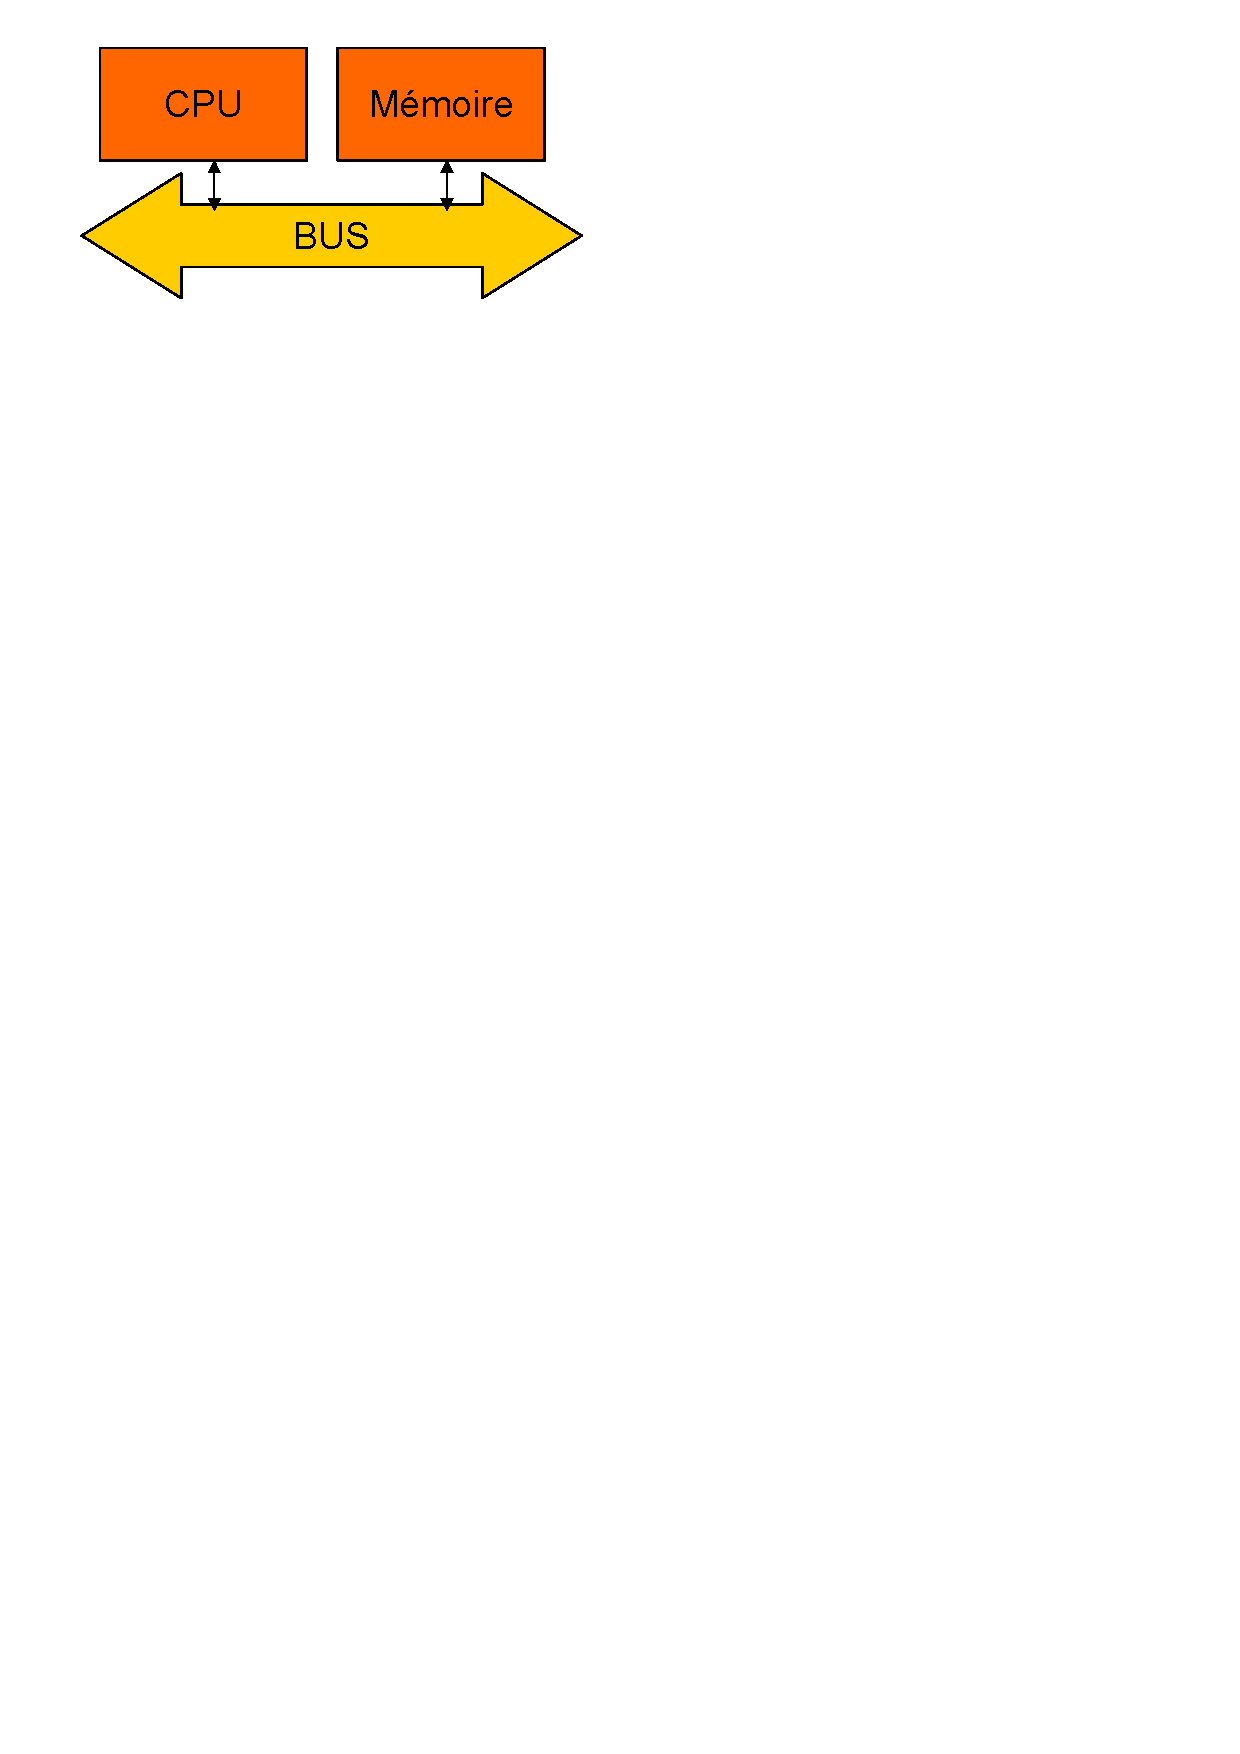
\includegraphics[height=2cm]{../illustration/vn_cpu_mem_bus.pdf}
\end{frame}


\begin{frame}
\frametitle{Composition d'un processeur}
\begin{itemize}
\item <1> [ALU] Unité Arithmétique et Logique. Prend en charge les calculs arithmétiques élémentaires et les tests \cite{wp-cpu}
\item <2> [UC] Unité de contrôle ou séquenceur. Permet de synchroniser les différents éléments du processeur
\item <3> [Registres] Mémoires de petite taille (quelques octets), suffisamment rapides pour que l'UAL puisse manipuler leur contenu à chaque cycle de l’horloge
\item <4> [Horloge] Synchronise toutes les actions de l’unité centrale (processeurs synchrones)
\item <5> [Unité E/S] Prend en charge la communication avec 
\begin{itemize}
\item la mémoire de l’ordinateur
\item les périphériques de l’ordinateur
\end{itemize}
\end{itemize}

\end{frame}

\begin{frame}
\frametitle{L'architecture Von Neumann}
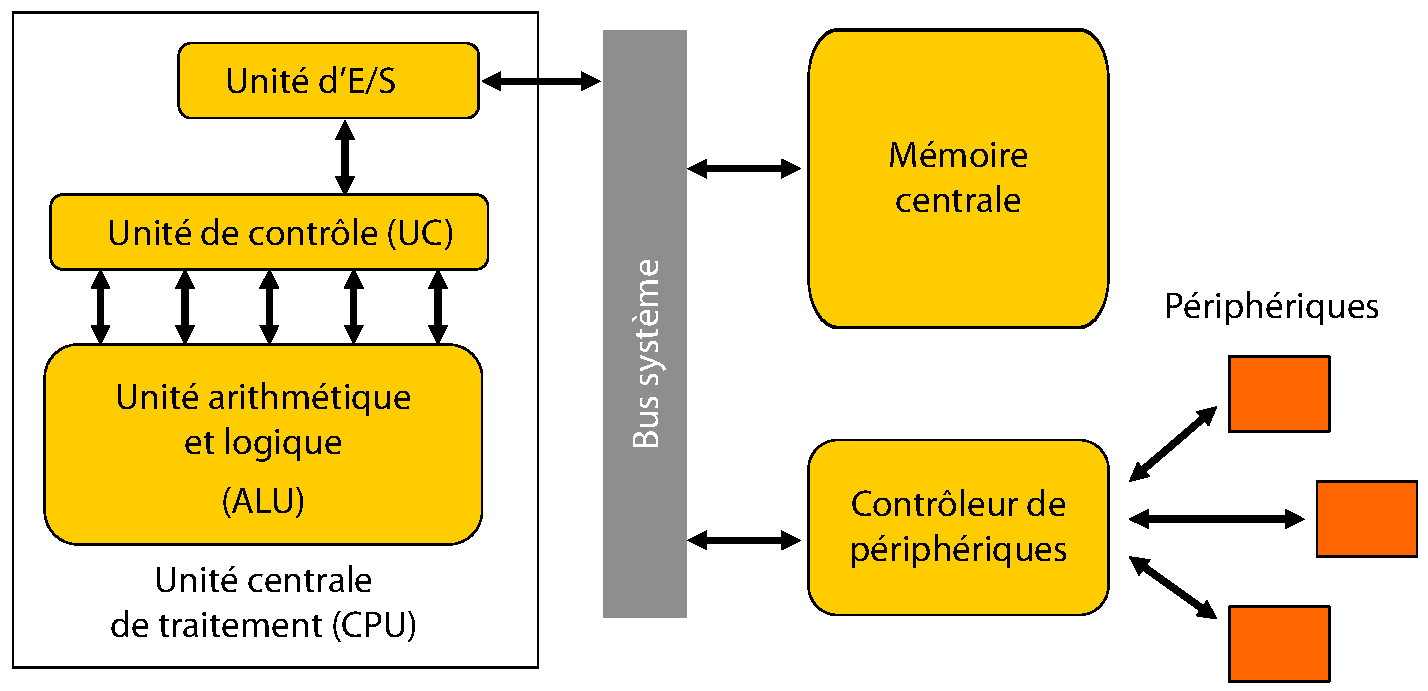
\includegraphics[height=5cm]{../illustration/archi_von_neumann.pdf}
\end{frame}

\begin{frame}
\frametitle{Le rôle du processeur (CPU)}
\begin{itemize}
\item Traiter les instructions :
\begin{itemize}
\item Exécuter les instructions
\item Réalise des traitements séquentiels
\end {itemize}
\item Manipuler les données
\begin{itemize}
\item Lire séquentiellement des instructions pointées dans la mémoire par le compteur ordinal (CO)
\item Lire éventuellement les opérandes stockées dans la mémoire
\item Placer éventuellement en mémoire le résultat du traitement
\end{itemize}
\item Communiquer avec les périphériques et le monde extérieur
\end{itemize}
\end{frame}


\begin{frame}
\frametitle{Déroulement d'un programme}
\begin{itemize}
\item Le processeur exécute des instructions élémentaires 
\begin{itemize}
\item En séquence sauf en cas de saut
\end{itemize}
\item Contrôlé par le Compteur Ordinal (CO)
\begin{itemize}
\item Prochaine instruction à exécuter
\item Certaines instructions peuvent modifier directement le CO (saut)
\end{itemize}
\item Instructions amenées une à une vers le processeur
\end{itemize}
\end{frame}


\begin{frame}
\frametitle{Séquencement des instructions}
\begin{itemize}
\item Instruction composée de plusieurs étapes
\begin{itemize}
\item Micro-instructions
\end{itemize}
\item Type d'action :
\begin{itemize}
\item Activité mémoire
\item Activité processeur
\end{itemize}
\item Cycle processeur
\begin{itemize}
\item Phase de chargement $\rightarrow$ fetch
\item Phase d'exécution $\rightarrow$ exec
\end{itemize}
\end{itemize}
\end{frame}


\begin{frame}
\frametitle{Séquencement des instructions}
\begin{figure}[htbp]
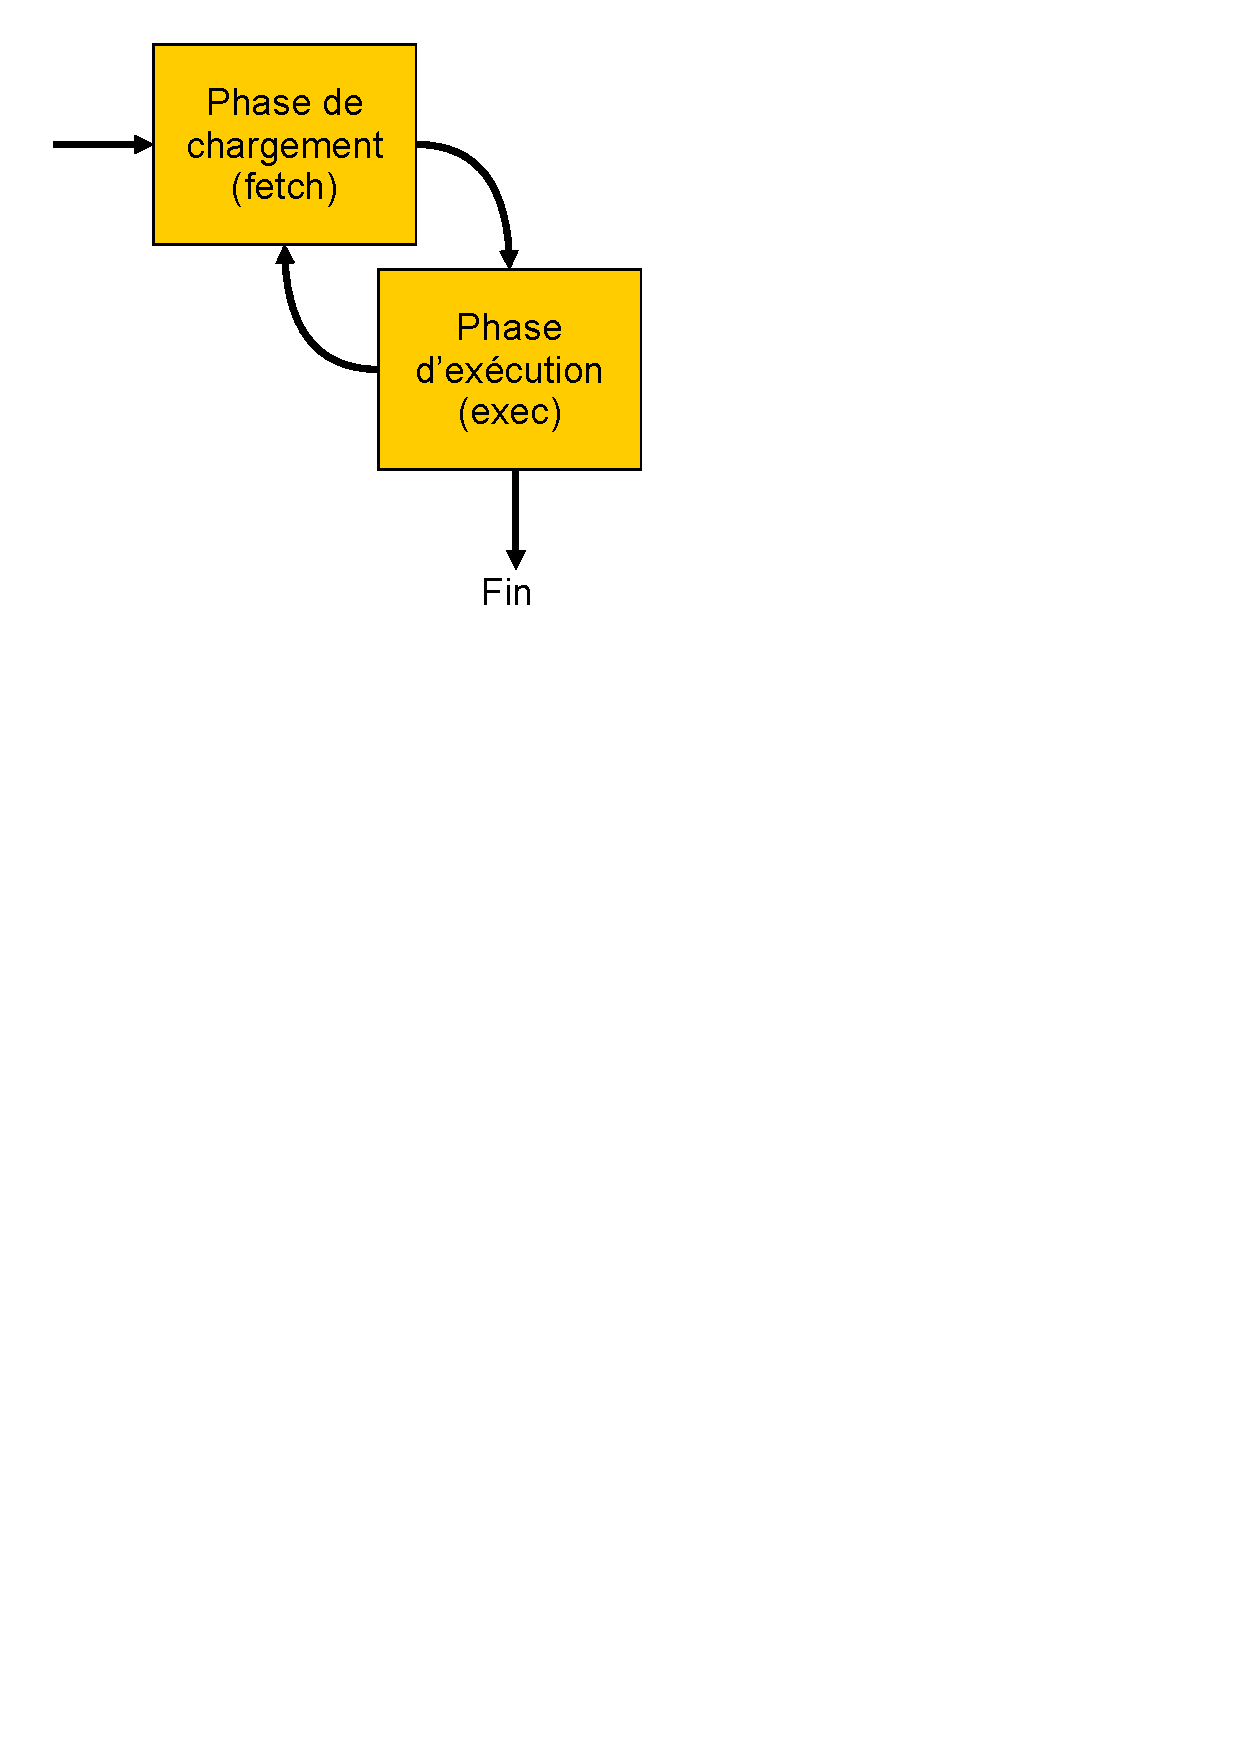
\includegraphics[height=5cm]{../illustration/phases_exec.pdf}
\end{figure}
\end{frame}


\begin{frame}
\frametitle{Séquencement des instructions (Von Neumann)}
Prise en compte des instructions en cinq étapes :
\begin{itemize}
\item <1>[IF \footnote{Instruction \texttt{Fetch}}] Lecture de l'instruction depuis la mémoire
\item <2>[ID\footnote{Instruction \texttt{Decoding}}] Décodage de l'instruction et recherche des opérandes (registre ou valeurs immédiate)
\item <3>[EX] Exécution de l'instruction (EXexute)
\item <4>[\textit{MEM}] \textit{Accès mémoire, écriture dans la mémoire si nécessaire ou chargement depuis la mémoire - facultatif}
\item <5>[WB\footnote{\texttt{Write Back}}] Ecriture de la valeur calculée dans les registres
\end{itemize}
\end{frame}



\begin{frame}
\frametitle{Exécution d'un programme}
\begin{figure}[htbp]
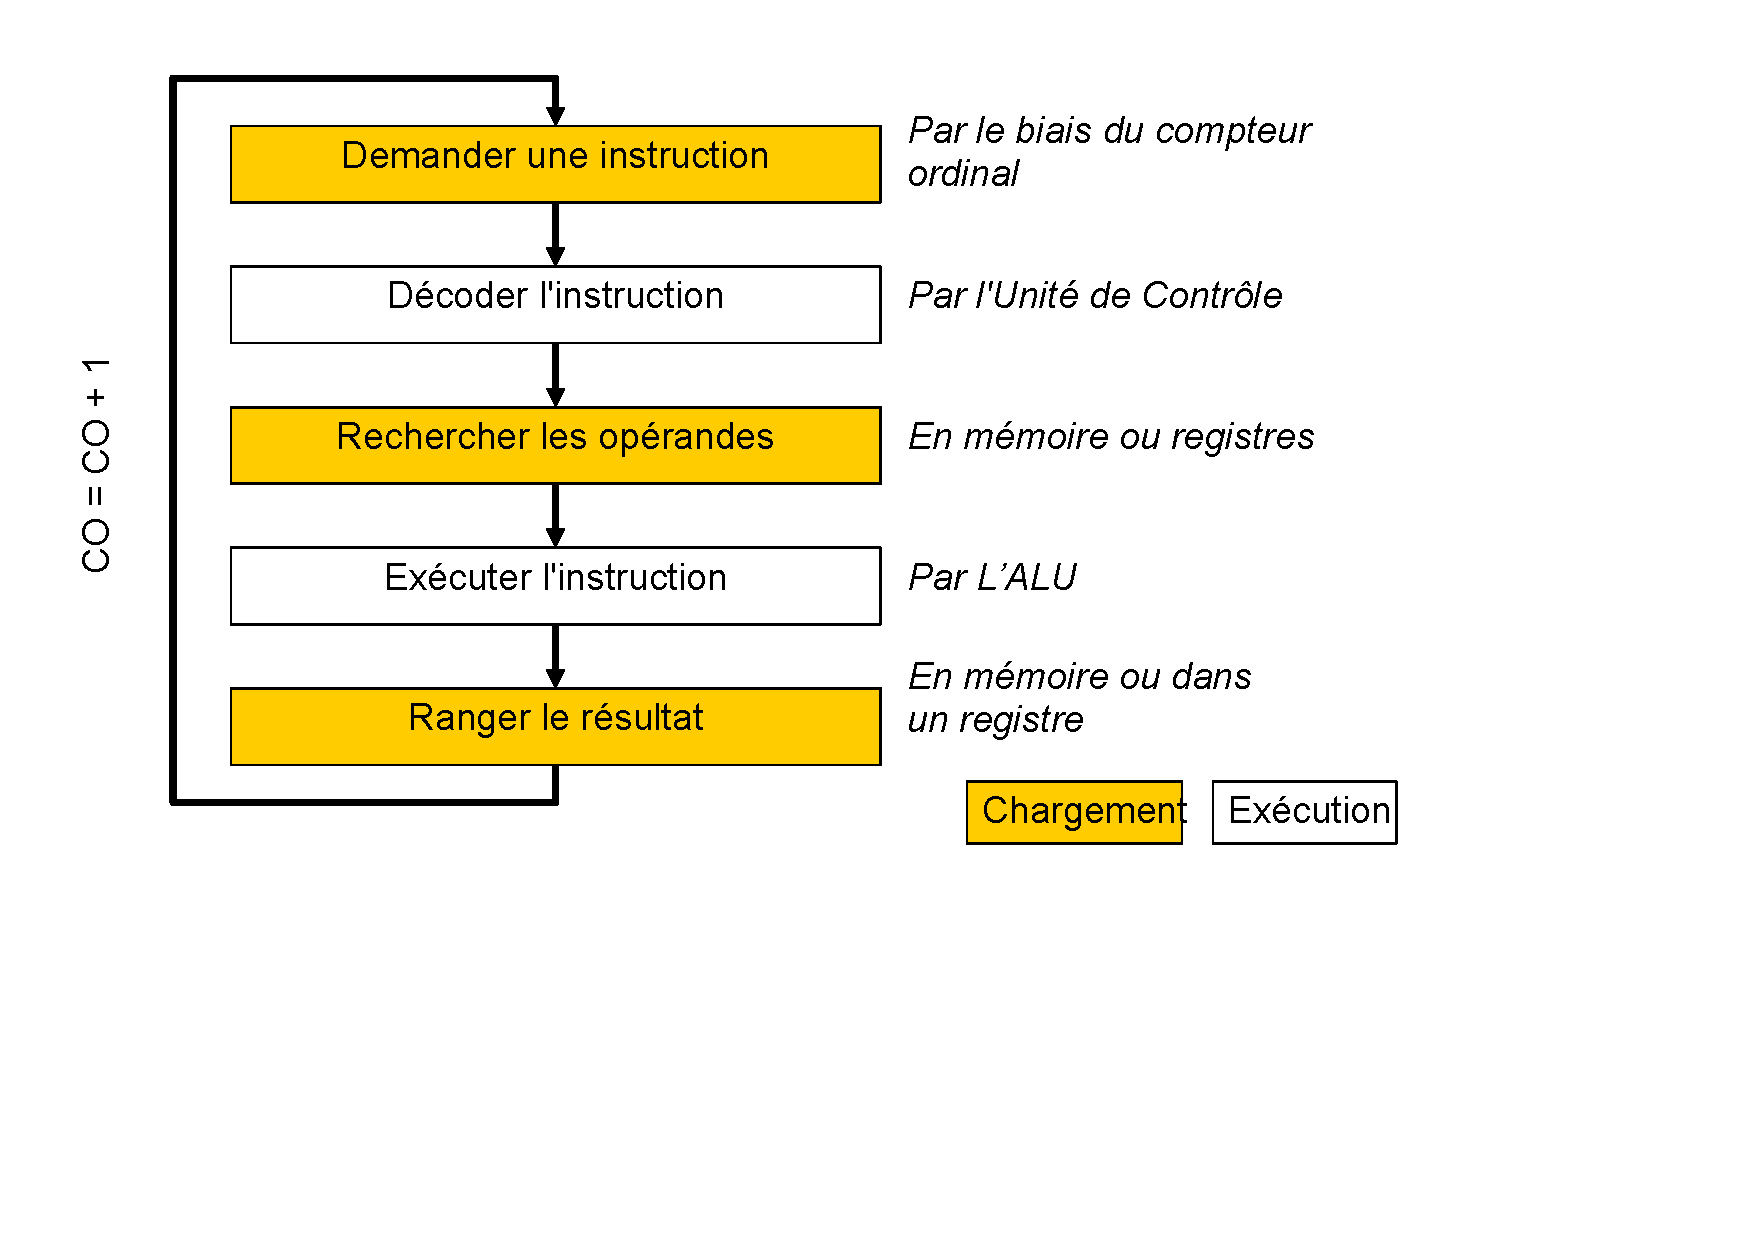
\includegraphics[height=5cm]{../illustration/exec_pgm.pdf}
\end{figure}
\end{frame}

\begin{frame}
\frametitle{Alternative : architecture Harvard \cite{wp-harvard}}
\begin{itemize}
\item Mise en œuvre par l'Université de Harvard pour le Mark I (1944)
\item Différences avec l'architecture Von Neumann :
\begin{itemize}
\item Spécialisation de la mémoire entre données et instructions
\item Transferts simultané, en parallèle 
\item Gain de performance, mais plus grande complexité
\end{itemize}
\end{itemize}
\begin{exampleblock}{Mise en œuvre}
\begin{itemize}
\item processeurs numériques de signal (DSP) ;
\item microcontrôleurs (PIC de Microchip, AVR d'Atmel).
\end{itemize}

\end{exampleblock}

\end{frame}


\subsection{Fonctionnement subscalaire / superscalaire}

\begin{frame}
\frametitle{Fonctionnement subscalaire}
\begin{itemize}
\item  Forme la plus simple que peut prendre un CPU
\item Une seule instruction n'est exécutée à la fois
\item Composantes du CPU sous utilisés :
\begin{itemize}
\item Il faut 15 cycles pour exécuter trois instructions
\end{itemize}
\end{itemize}
\begin{figure}
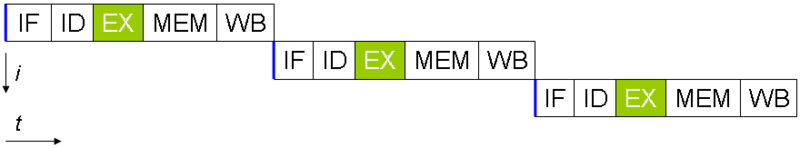
\includegraphics[width=10cm]{../illustration/processeur-fonc_subscalaire.png}
\caption{Extrait de \cite{wp-cpu}}
\end{figure}
\end{frame}

\begin{frame}
\frametitle{Fonctionnement superscalaire}
\begin{block}{Objectif}
\begin{itemize}
\item Comportement moins linéaire et plus parallèle du CPU
\item Optimisation des capacités d'exécution
\end{itemize}
\end{block}
\begin{itemize}
\item Utilisation d'un \textbf{pipeline} d'instructions \index{pipeline}
\item Parallélisme de processeur :
\begin{itemize}
\item Instruction Level Parallelism (ILP) \index{ILP}
\begin{itemize}
\item Parallélisme au niveau instruction
\end{itemize}
\item Thread Level Parallelism (TLP)  \index{TLP}
\begin{itemize}
\item Parallélisme au niveau thread (groupe d'instructions)
\end{itemize}
\end{itemize}
\end{itemize}
\end{frame}

\begin{frame}
\frametitle{Fonctionnement superscalaire ILP}
\begin{itemize}
\item Principe du travail à la chaine
\item Améliorer l'utilisation des ressources d'exécution
\end{itemize}
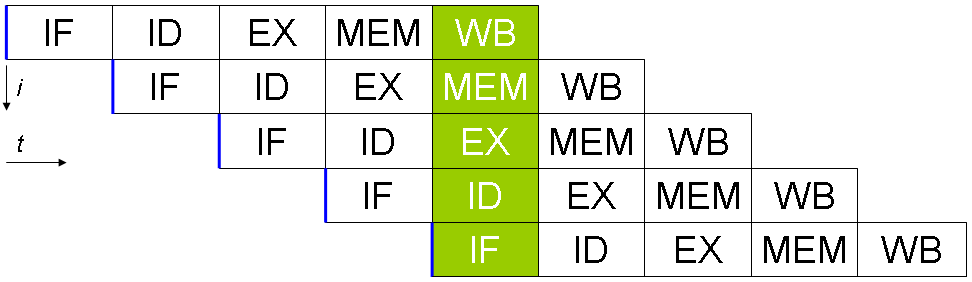
\includegraphics[width=10cm]{../illustration/processeur-ILP.png}

Un pipeline de base à 5 étages\footnote{Comme celui de l'Intel 486} peut soutenir un taux d'exécution d'une instruction par cycle. \cite{wp-cpu}
\end{frame}

\begin{frame}
\frametitle{Fonctionnement superscalaire TLP}
\begin{itemize}
\item Capacité d'exécuter plusieurs programmes simultanément
\begin{itemize}
\item \textit{Multithreading processeur}
\item Comportement équivalent à un système multi-processeurs
\item Optimisation de l'usage des unités d'exécution (ALU)
\end{itemize}
\item Duplication de certaines parties du CPU (le moins possible) :
\begin{itemize}
\item la recherche $\rightarrow$ fetch
\item le décodage $\rightarrow$ decode
\item la répartition des instructions $\rightarrow$ dispatch
\item les registres non spécialisés.
\end{itemize}
\item Mis en œuvre dès 1950 
\end{itemize}
\end{frame}

\begin{frame}
\frametitle{Fonctionnement superscalaire TLP}
En recherchant et affectant deux instructions à la fois, le CPU peut exécuter un maximum de deux instructions par cycle \cite{wp-cpu}
\begin{figure}
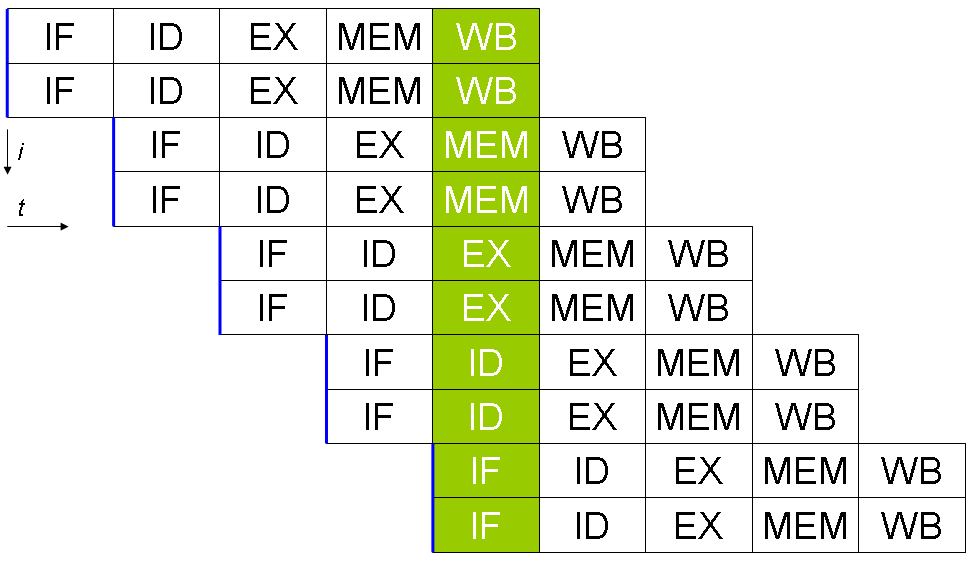
\includegraphics[height=5cm]{../illustration/Superscalarpipeline.png}
\end{figure}
\end{frame}


\subsection{Interruptions - Gestion des périphériques}

\begin{frame}
 \frametitle{Composition d’un système informatique moderne}
 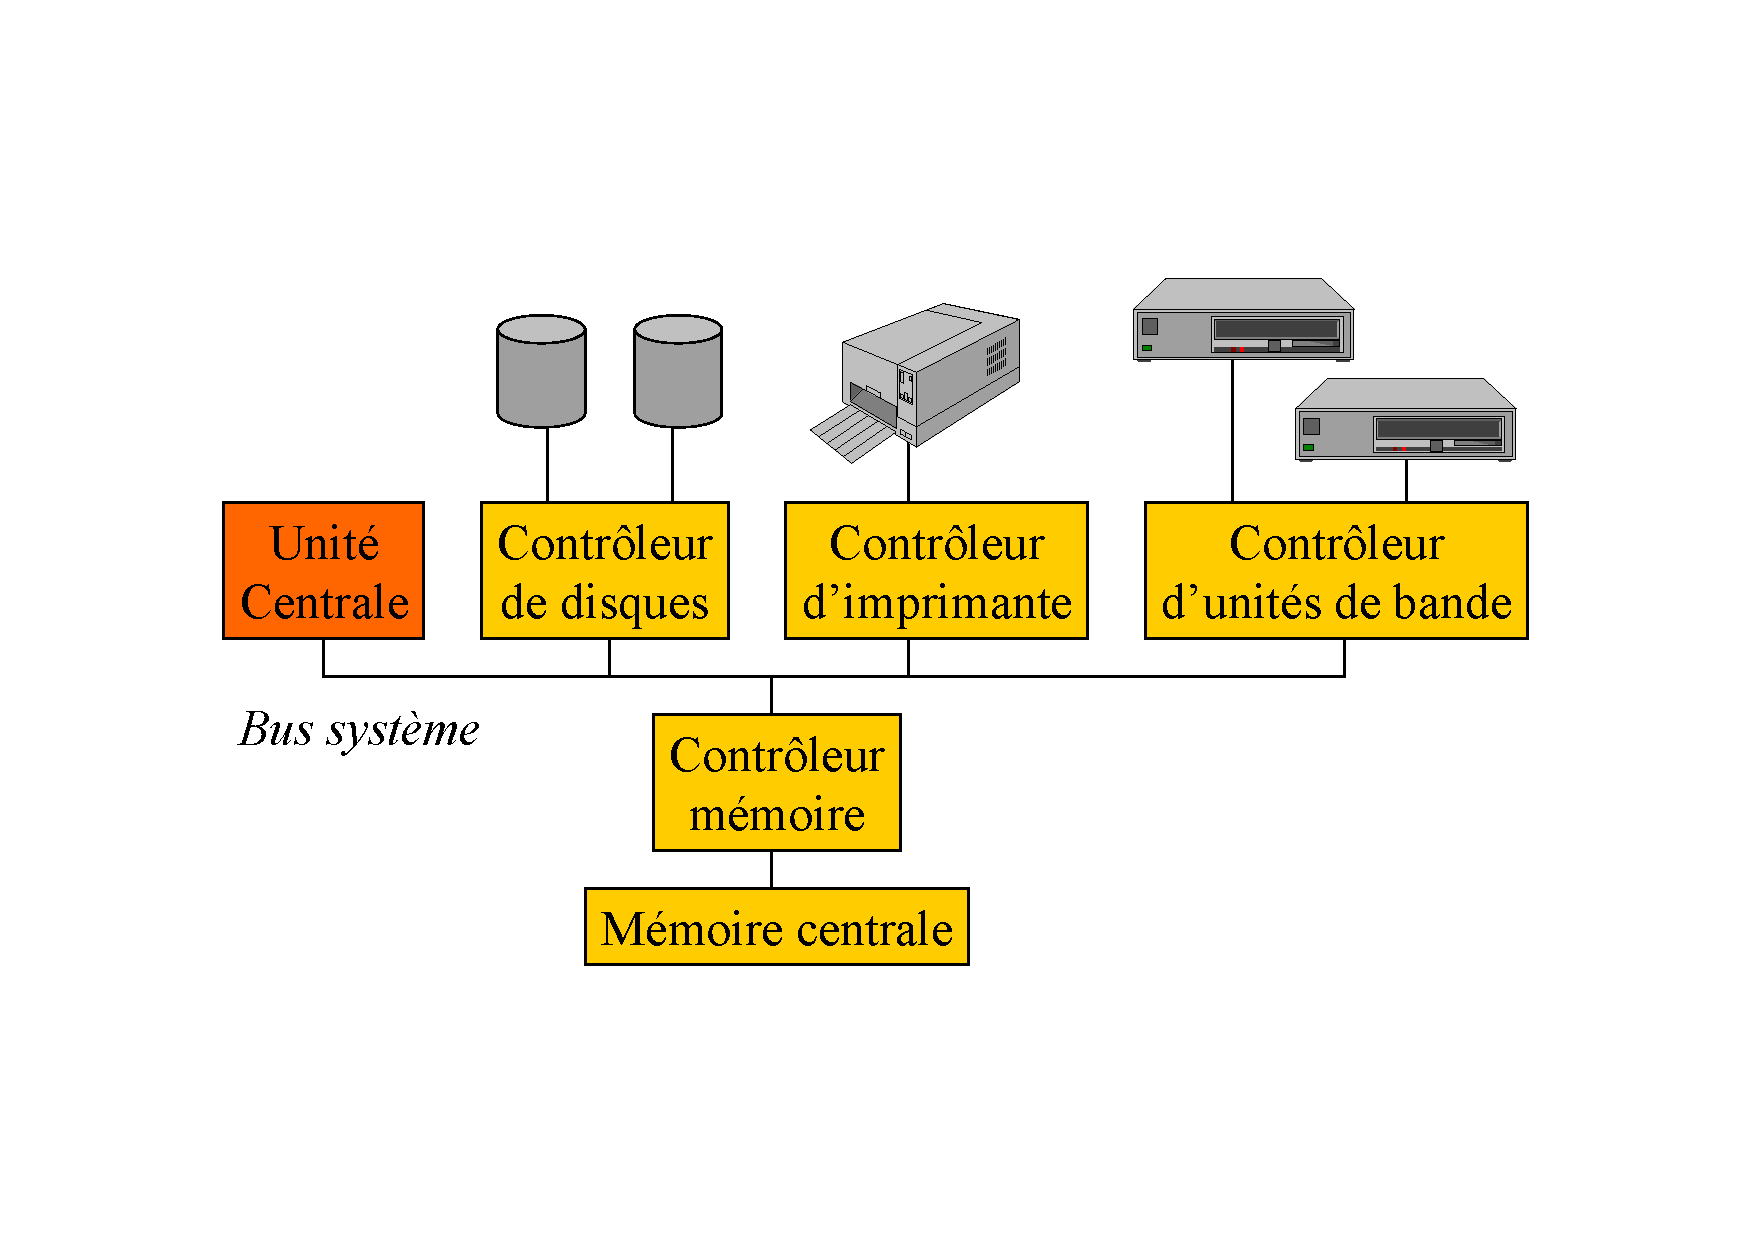
\includegraphics[width=\textwidth]{../illustration/archi_si.pdf}
\end{frame}


\begin{frame}
\frametitle{Séquence de démarrage}
Prise en charge par le programme d’amorçage :
\begin{itemize}
\item Initialisation du matériel
\begin{itemize}
\item registres du processeur,
\item contrôleurs de périphériques,
\item mémoire...
\end{itemize}
\item Chargement du système d’exploitation
\begin{itemize}
\item Exécution des premiers processus (initialisation)
\end{itemize}
\item Attente d’un évènement...
\end{itemize}
\end{frame}



\begin{frame}
\frametitle{Séquence de démarrage}
\begin{itemize}
\item Prise en charge par le programme d'amorçage
\item BIOS : Basic Input Output System \cite{wp-bios}
\begin{itemize}
\item Mis en place pour les premiers PC
\item Limité (accès mémoire, partiellement 16 bits, pas d'accès réseau...) et difficilement portable
\item Inadapté aux architectures 64 bits et aux besoins de télégestion
\end{itemize}

\item UEFI : Unified Extensible Firmware Interface \cite{wp-uefi} - Intel
\begin{itemize}
\item Interface micrologicielle extensible unifiée (modulaire et interaction possible avec l'OS)
\item fonctionnalités réseau intégrées en standard
\item écrit en C, plus portable et maintenable :  Itanium (IA-64), x86 (32bits et 64bits) et ARM
\end{itemize}
\end{itemize}
\end{frame}



\begin{frame}
\frametitle{Évènements et interruptions}
Signalés par une interruption :
\begin{itemize}
\item Matérielle
\begin{itemize}
\item envoyée par un contrôleur de périphérique
\item utilise le bus système
\item peut être masquée\footnote{interruptions masquables} ou invalidée 
\end{itemize}
\item Logicielle
\begin{itemize}
\item semblables aux interruptions matérielles
\item émises par des programmes
\item ne peut être ni invalidé ni masquée
\end{itemize}
\end{itemize}
\end{frame}



\begin{frame}
\frametitle{Exemples d'interruptions}
\begin{columns}
\column{.5\textwidth}
\begin{exampleblock}{Interruptions materielles}
\begin{itemize}
\item Erreur
\begin{itemize}
\item accès mémoire incorrect
\end{itemize}
\item E/S
\begin{itemize}
\item fond de lecture ou d'écriture sur disque
\end{itemize}

\item Interaction utilisateur
\begin{itemize}
\item frappe clavier
\item déplacement souris
\item CTRL + ALT + SUPPR
\end{itemize}
\item Horloge
\item ...
\end{itemize}

\end{exampleblock}
\column{.5\textwidth}
\begin{exampleblock}{Interruptions logicielles}
\begin{itemize}
\item Lecture de l'horloge temps réel
\item Appel au superviseur (appel système)
\item Demande d'E/S
\item Division par zéro
\end{itemize}

\end{exampleblock}
\end{columns}
\end{frame}

\begin{frame}
 \frametitle{Traitement d’une interruption}
 Traités par une routine système :
\begin{itemize}
\item Arrêt travail en cours
\item Transfert de l’exécution sur la routine de traitement (emplacement fixe)
\begin{itemize}
\item qualification de l’interruption
\item traitement
\end{itemize}
\item Transfert de l’exécution sur le dispatcher
\end{itemize}
\end{frame}


\begin{frame}
 \frametitle{Les interruptions}
 \begin{itemize}
 \item Partie importante de l’architecture d’un ordinateur
\begin{itemize}
\item Doivent être traitées très rapidement
\end{itemize}
\item Nombre prédéfini d’interruptions possibles
\begin{itemize}
\item Table de pointeurs vers des routines de traitement
\begin{itemize}
\item Vecteur d’interruption
\item Généralement stockée au tout début de la mémoire de l'ordinateur, en $0000:0000$
\end{itemize}
\item Pas de routine intermédiaire
\end{itemize}
 \end{itemize}
\end{frame}


\begin{frame}
 \frametitle{Appel indirect de routine de traitement d’interruption}
 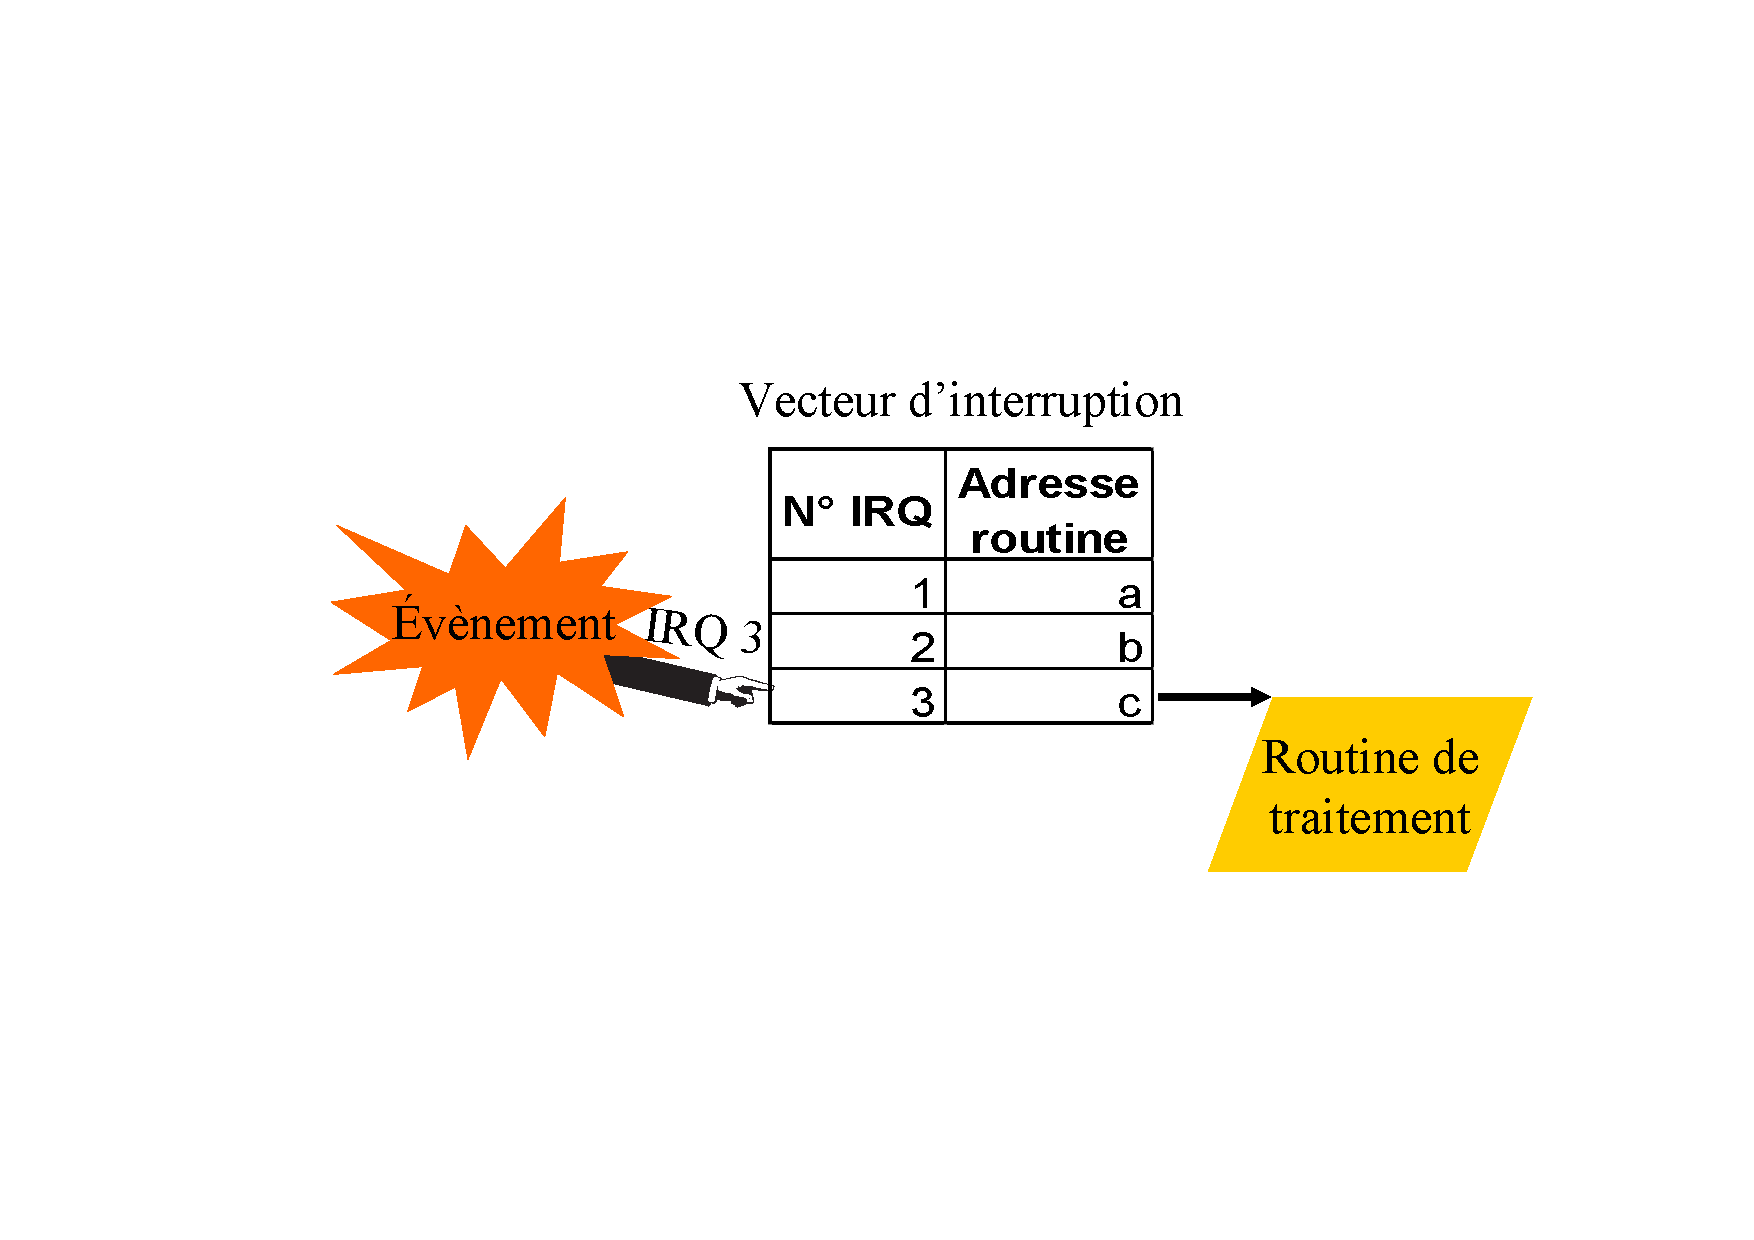
\includegraphics[width=\textwidth]{../illustration/derout_interruption.pdf}
\end{frame}


\begin{frame}
 \frametitle{Influence sur la structure du système}
 \begin{itemize}
 \item Systèmes modernes dits \textbf{dirigés par les interruptions}
 \item Influence la structure générale d’un système d’exploitation
 \item Chaque type d’interruption est traité par une partie du système
 \end{itemize}
\end{frame}


\begin{frame}{Les différents niveaux de bus}
Sur les premiers systèmes :
\begin{itemize}
\item Un bus unique
\begin{itemize}
\item connexion de tous les composants 
\item mémoire, dispositifs d'E/S...
\end{itemize}
\item Priorité des contrôleurs d'E/S sur le processeur
\begin{itemize}
\item risque de perdre des informations
\begin{itemize}
\item faible capacité de stockage au niveau du contrôleur
\end{itemize}

\item perte de cycle pour le processeur
\item vol de cycle (\textit{cycle stealing})
\end{itemize}
\item Acceptable tant que les performances des composants restent homogènes
\end{itemize}
\end{frame}


\begin{frame}{Les différents niveaux de bus}
\begin{itemize}
\item Sur les systèmes actuels :
  \begin{itemize}
    \item Grande disparité des performances
      \begin{itemize}
        \item mémoire, disque, réseau, carte graphique...
      \end{itemize}
    \item Important débits d'E/S
  \end{itemize}
    \item Solution :
    \begin{itemize}
	\item Bus plus rapide (stations de travail)
    \end{itemize}


  \item Problème de la rétro-compatibilité :
  \begin{itemize}
    \item Assurer la compatibilité avec les anciens matériels (PS/2)
    \item Plusieurs niveaux de bus, par ordre décroissant de performance
    \begin{itemize}
      \item bus mémoire
      \item bus PCI
      \item bus ISA
    \end{itemize}
  \end{itemize}
\end{itemize}
\end{frame}


\begin{frame}{Les différents niveaux de bus}
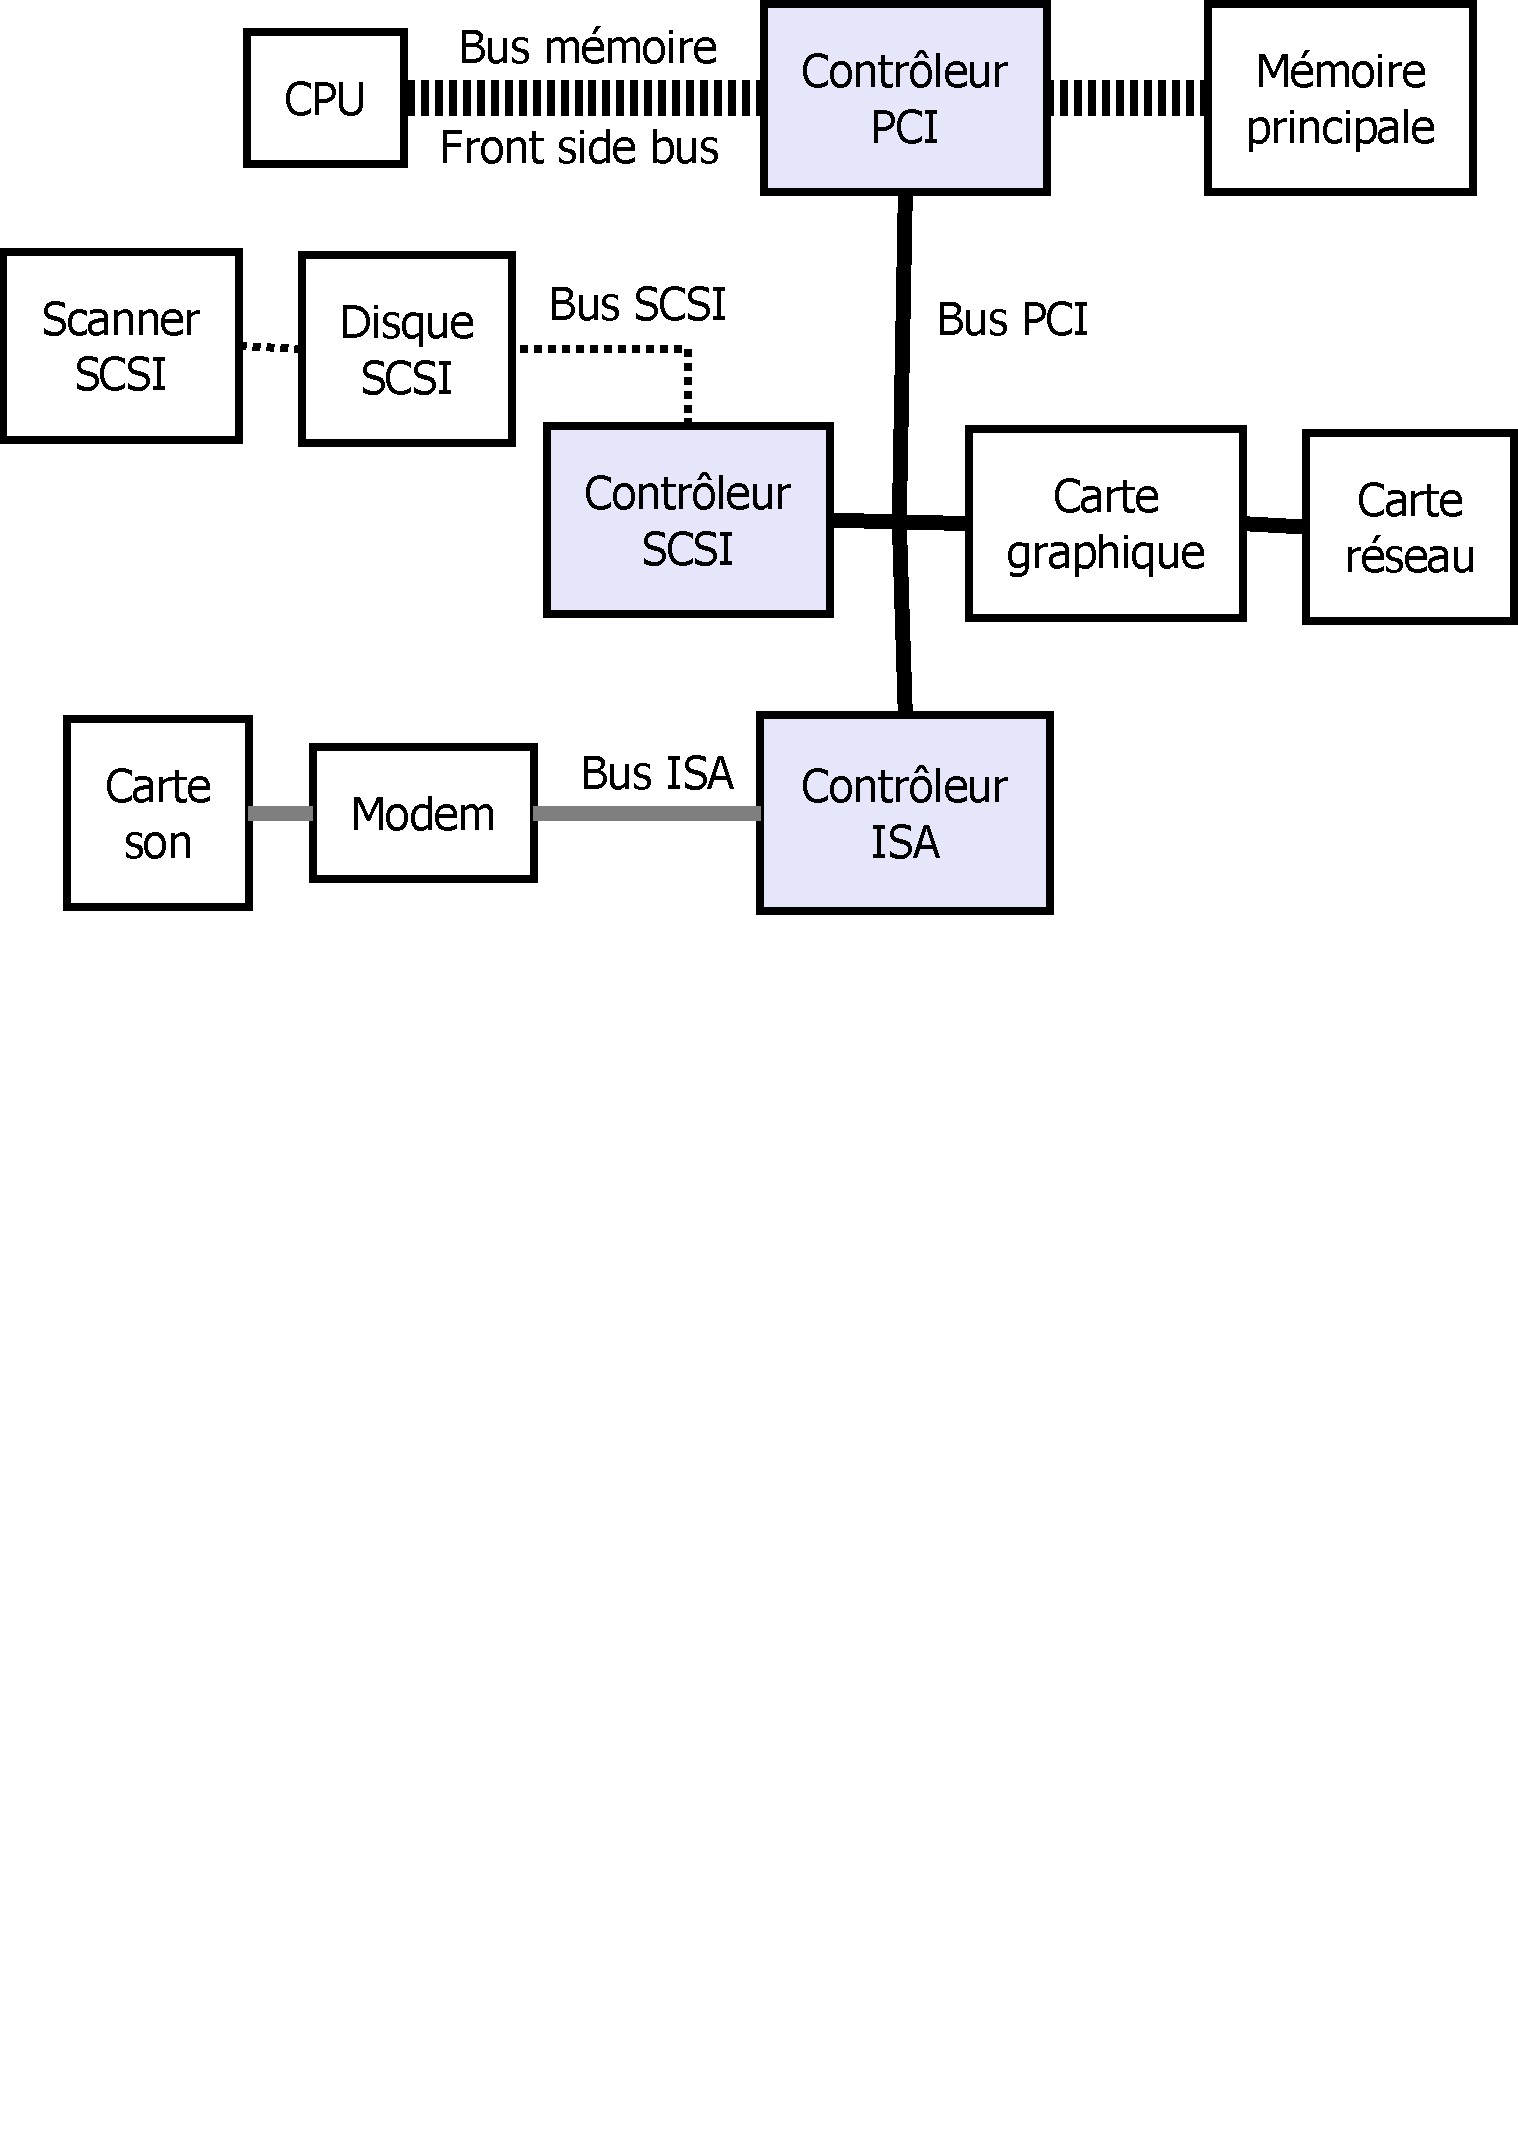
\includegraphics[width=\textwidth]{../illustration/NiveauxBus.pdf}
\end{frame}


\begin{frame}{ARM : bus CoreLink CCN-504}
Bande passante de 1 To/s \cite{xbits}
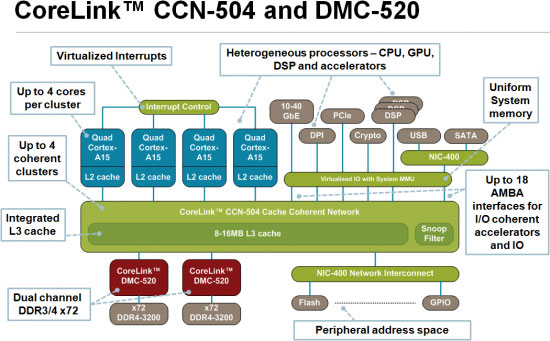
\includegraphics[width=\textwidth]{../illustration/arm504.jpg}
\end{frame}

\begin{frame}
 \frametitle{Interruptions matérielles du x86 : modèle PIC}
 \begin{itemize}
 \item \textit{Programmable Interrupt Controler}
 \item 15 interruptions matérielles : les IRQ, ou Interruption Request
\begin{itemize}
\item Assignées au matériel :
\begin{itemize}
\item le processeur, la mémoire, les cartes d'extension, les périphériques, l'horloge, etc...
\end{itemize}
\item Quantité limitée
\begin{itemize}
\item partage nécessaire
\item risque de conflits
\end{itemize}
\item Systématiquement associée à une interruption logicielle
\end{itemize}
\end{itemize}
\end{frame}

\begin{frame}
\frametitle{Interruptions matérielles du x86 : modèle PIC}
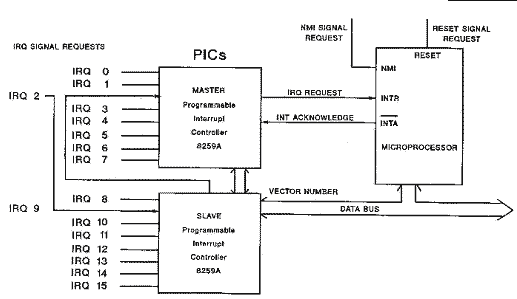
\includegraphics[width=.8\textwidth]{../illustration/interruption_PIC.png}
\end{frame}


\begin{frame}
 \frametitle{Les 15 interruptions matérielles du x86 (modèle PIC)}
 \begin{small}
 \begin{tabular}{c|l}
  IRQ 0 & System Timer \\
  IRQ 1 & Clavier \\
  IRQ 3 & COM2 (second port série) \\
  IRQ 4 & COM1 (premier port série) \\
  IRQ 5 &  "disponible" (souvent utilisée pour la carte son) \\
  IRQ 6 & Lecteur de disquettes (2 maximum) \\
  IRQ 7 & LPT1 (le port parallèle) \\
  IRQ 8 & Real Time Clock (horloge temps réel) \\
  IRQ 9 &  "disponible" \\
  IRQ 10 & "disponible" \\
  IRQ 11 & "disponible" \\
  IRQ 12 & Souris PS/2 \\
  IRQ 13 & Coprocesseur arithmétique \\
  IRQ 14 & Canal IDE primaire (2 maximum) \\
  IRQ 15 & Canal IDE secondaire (2 maximum)
 \end{tabular}
\end{small}
\end{frame}
 
\begin{frame}
\frametitle{Interruptions matérielles du x86 (modèle APIC)}
\begin{itemize}
\item \textit{Advanced Programmable Interrupt Controler}
\item Géré par le BIOS
\item En complément du PIC standard
\item 256 interruptions
\begin{itemize}
\item Intègre les 16 du modèle PIC (liées à une IRQ)
\item Défini dans le \textbf{vecteur d'interruption}
\end{itemize}
\item Indispensable pour le SMP
\begin{itemize}
\item Traitement individuel des CPU à interrompre
\end{itemize}
\item Imposé par Windows XP
\begin{itemize}
\item même sur les machines mono-processeur
\begin{figure}[b!]

\includegraphics[height=1cm]{../illustration/logo_windowsXP.png}
\end{figure}
\end{itemize}
\end{itemize}
\end{frame}

\begin{frame}
\frametitle{Modèle APIC}
\begin{itemize}
\item Communication via le \textbf{bus APIC}
\begin{itemize}
\item Bus logique
\end{itemize}
\item Local APIC
\begin{itemize}
\item Propre à chaque processeur
\item Gère les interruptions locales pour le processeur local
\end{itemize}
\item IO-APIC
\begin{itemize}
\item Redirige les interruptions
\begin{itemize}
\item d'un APIC local vers un autre
\item vers un autre IO-APIC
\end{itemize}
\item Table de redirections
\item Plusieurs I/O APIC répartis dans le reste du système (PCI...)
\end{itemize}
\end{itemize}
\end{frame}


\begin{frame}
\frametitle{Les entrées - sorties}
\begin{itemize}
\item Matériel d'E/S
\item Scrutation
\item Les interruptions
\item Accès direct en mémoire
\item Périphériques
\item Gestion des requêtes d'E/S
\end{itemize}
\end{frame}



\begin{frame}
\frametitle{Les périphériques d’E/S}
\begin{itemize}
\item Périphériques connectés par un bus
\item Pilotés par un contrôleur
\begin{itemize}
\item registres propres
\item mémoire tampon
\item pilote plusieurs périphériques de même type
\item responsable des déplacements entre périphériques et mémoire tampon
\end{itemize}
\item Capable de lever des interruptions
\end{itemize}
\end{frame}


\begin{frame}
\frametitle{La scrutation d'E/S}
\begin{itemize}
\item Attente active
\item Teste constamment si l'E/S est réalisée
\begin{itemize}
\item place des structures de contrôle en mémoire
\item observe leur contenu régulièrement
\item perte de cycles processeur
\end{itemize}
\item Transfert \textbf{synchrone}
\end{itemize}
\end{frame}


\begin{frame}
\frametitle{Interruption d’E/S}
\begin{itemize}
\item Contrôleur capable de lever des interruptions
\item Traitement d’une E/S :
\begin{itemize}
\item L’UC charge les registres du contrôleur
\item Le contrôleur examine ses registres
\item Démarrage du transfert des données vers ou depuis les registres du contrôleur
\item Information de l’UC de la fin du transfert
\end{itemize}
\item Transfert \textbf{asynchrone}
\end{itemize}
\end{frame}


\begin{frame}{Déroulement d'une E/S}
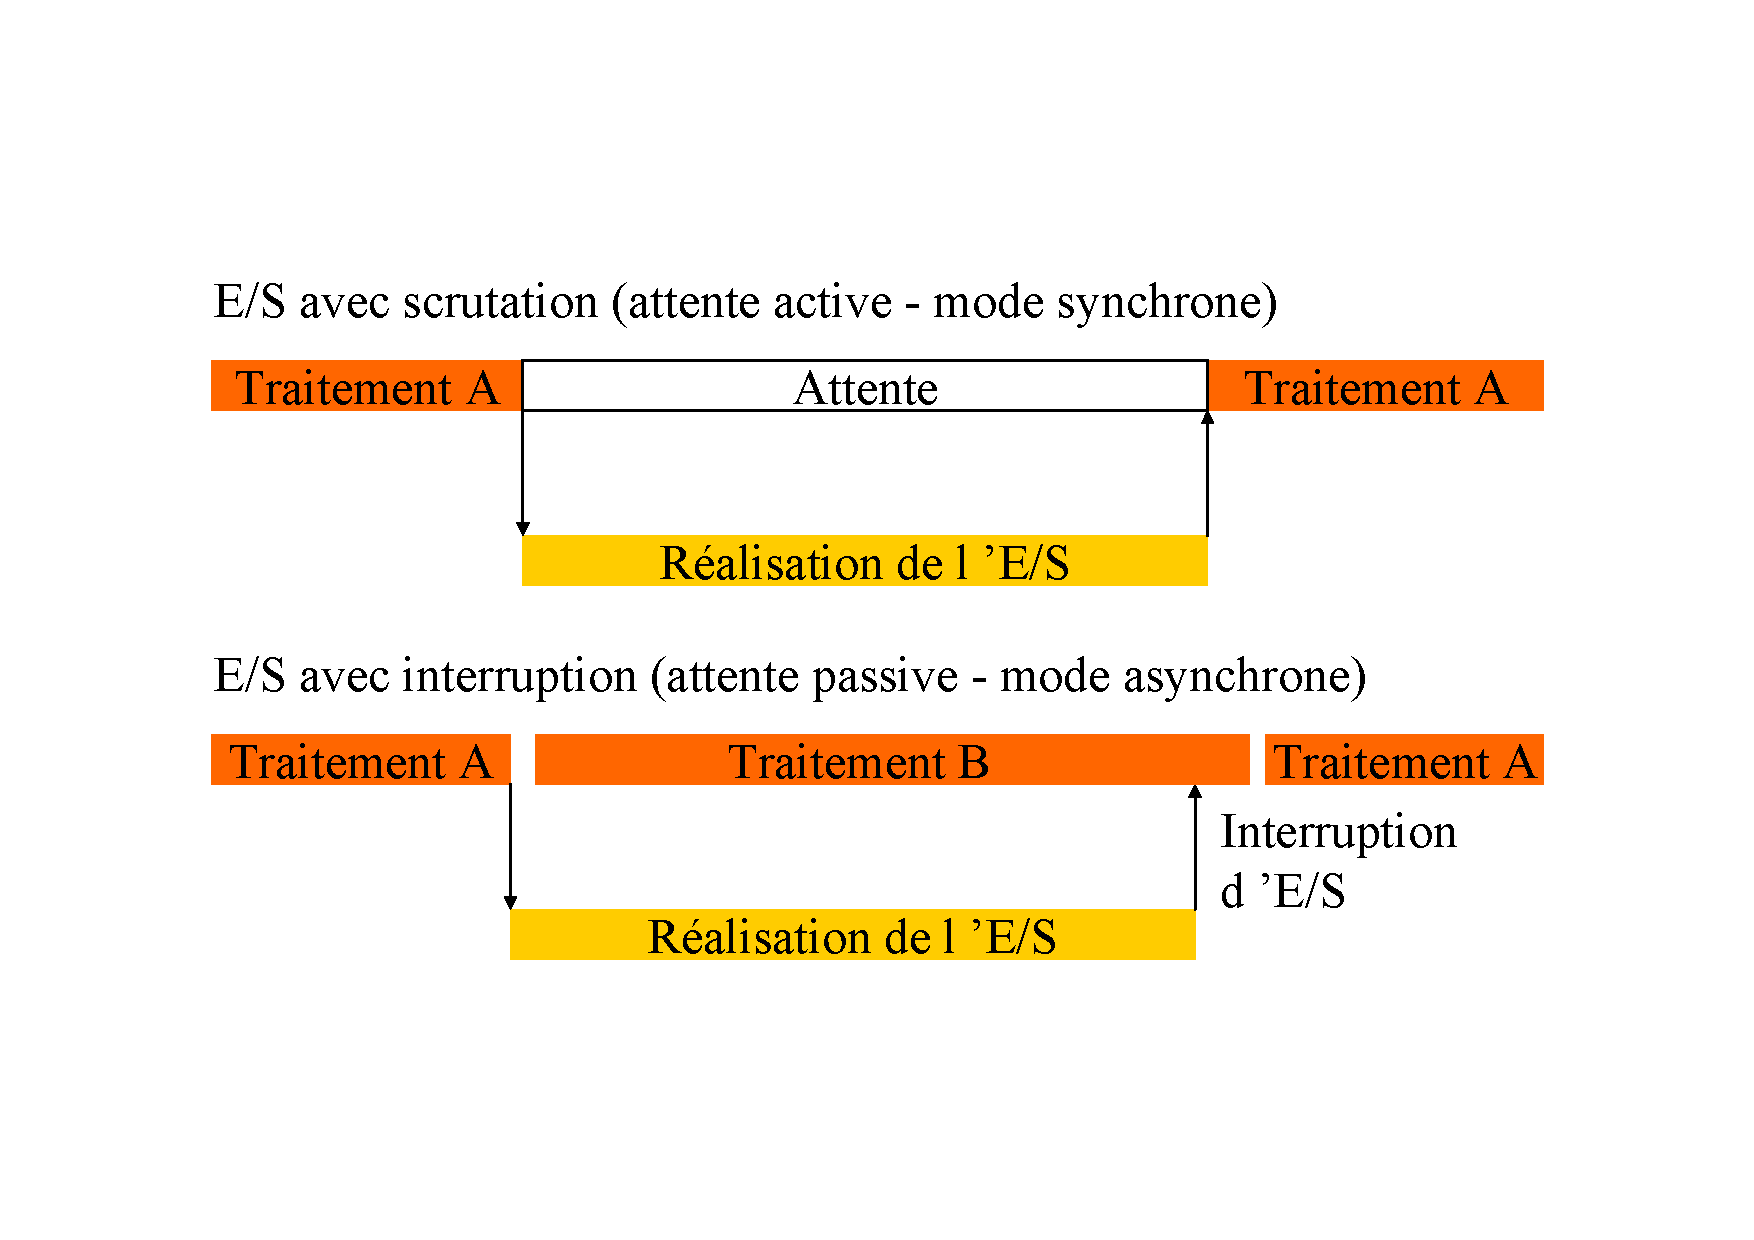
\includegraphics[width=\textwidth]{../illustration/Interruption_ES.pdf}
\end{frame}


\begin{frame}
\frametitle{Attente d’E/S}
\begin{itemize}
\item Attente active
\begin{itemize}
\item Boucle d’attente
\begin{itemize}
\item Attente interruption
\item Interrogation périphérique (drapeau)
\item Périphériques ne gérant pas les interruptions
\end{itemize}
\end{itemize}
\item Attente passive
\begin{itemize}
\item Attente interruption
\begin{itemize}
\item Instruction \texttt{wait}
\item Donne le contrôle à d’autres traitements
\end{itemize}
\end{itemize}
\end{itemize}
\end{frame}


\begin{frame}
\frametitle{File d’attente d’E/S}
\begin{itemize}
\item Une file d'attente par groupement de périphérique
\item Possibilité de suivre plusieurs requêtes d’E/S simultanément
\item Permet de connaître :
\begin{itemize}
\item Les périphériques disponibles
\item Leur adresse
\item Leur état (actif, inactif, indisponible)
\item La liste des travaux à traiter (file d’attente)
\end{itemize}
\end{itemize}
\end{frame}


\begin{frame}
\frametitle{Table de statut de périphérique}
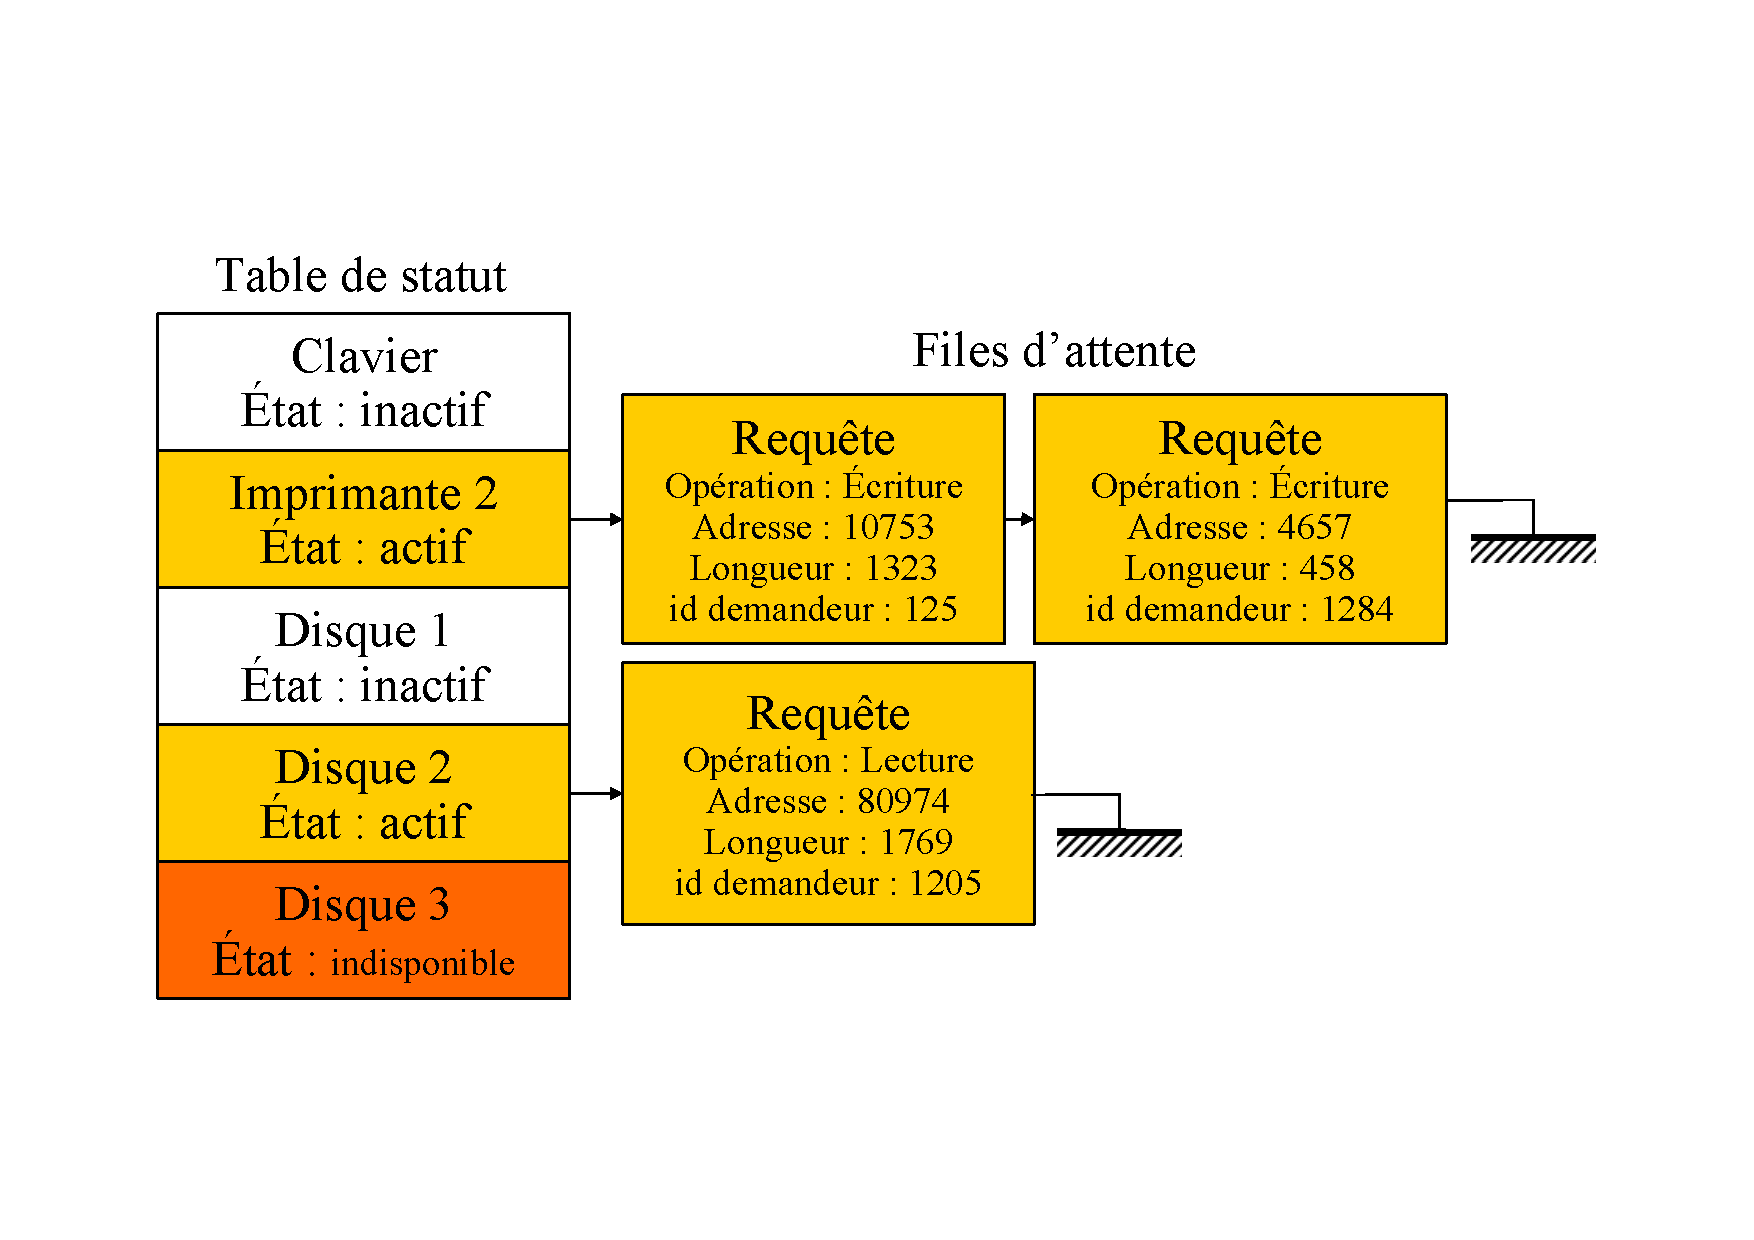
\includegraphics[width=\textwidth]{../illustration/table_statut.pdf}
\end{frame}


\begin{frame}
\frametitle{Traitement d’une interruption d’E/S}
\begin{itemize}
\item Interruption par un périphérique
\item Identification du périphérique demandeur (table des périphériques)
\item Identification du travail (file d’attente)
\begin{itemize}
\item Si le travail est terminé :
\begin{itemize}
\item Passage au travail suivant
\item Changement état du programme demandeur
\item Changement éventuel de l’état du périphérique
\end{itemize}
\item Sinon :
\begin{itemize}
\item Mise en place des directives pour la suite du travail
\item Lancement de l'E/S
\end{itemize}
\end{itemize}
\end{itemize}
\end{frame}


\begin{frame}
\frametitle{Cas d’une E/S non convoitée}
\begin{exampleblock}{Exemple : frappe en avance au clavier}
\begin{itemize}
\item Interruptions pour signaler l’arrivée de caractères
\item Aucun travail n’a requis de saisie clavier
\item Remplissage d’un tampon
\item Fourniture du contenu du tampon au prochain travail réclamant une entrée clavier
\end{itemize}
\end{exampleblock}
\end{frame}


\begin{frame}
\frametitle{Structure DMA}
\begin{block}{Problèmes à résoudre}
\begin{itemize}
\item Lenteur des E/S face à la CPU
\item Interruption de l’UC pour chaque mot
\end{itemize}
\end{block}
\begin{itemize}
\item Perte de cycles CPU
\item Solution proposée par DMA (Direct Memory Access)
\begin{itemize}
\item Processeur dédié au suivi des E/S :
\begin{itemize}
\item Communication directe du contrôleur avec la mémoire sans interruption de l’UC
\item Traitement de l’information par blocs (non par mot)
\end{itemize}
\item Utilisé par les périphériques rapides
\begin{itemize}
\item Processeur disponibles pour les calculs
\end{itemize}
\end{itemize}
\end{itemize}
\end{frame}


\begin{frame}
\frametitle{Structure DMA}
Traitement E/S :
\begin{itemize}
\item Configuration tampons, pointeurs, compteur en mémoire centrale (pilote) :
\begin{itemize}
\item Lecture $\rightarrow$ Tampon vide 
\item Ecriture $\rightarrow$ Tampon plein
\end{itemize}
\item Transfert direct en mémoire centrale des informations lues sur le périphérique (contrôleur), sans interruption de la CPU
\item Interruption lorsque le tampon est plein ou l’E/S terminée.
\end{itemize}
\end{frame}


\begin{frame}
\frametitle{Structure DMA}
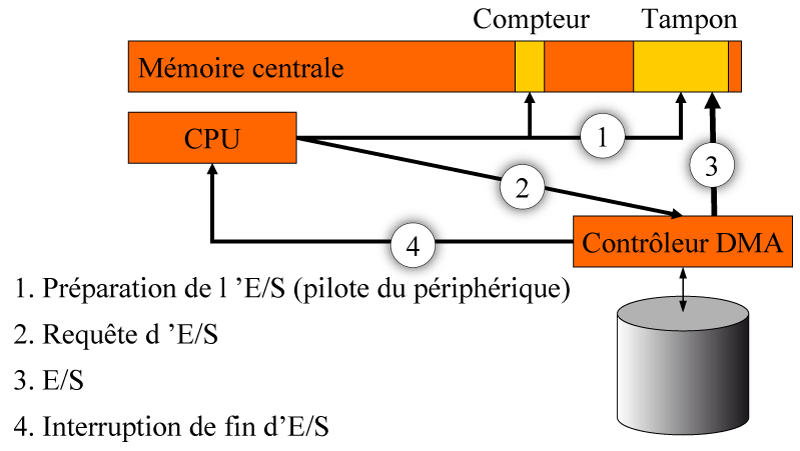
\includegraphics[width=\textwidth]{../illustration/traitement_DMA.png}
\end{frame}


\begin{frame}
\frametitle{Structure DMA}
\begin{itemize}
\item Accès direct à la mémoire centrale
\item E/S parallèle à d’autres travaux (sur CPU ou autre périphérique DMA)
\begin{itemize}
\item La mémoire ne peut écrire qu’un seul mot à la fois
\end{itemize}
\item Concurrence d’accès aux cycles mémoire
\begin{itemize}
\item Nécessité d’un contrôleur de mémoire
\item Ralentissement des accès mémoire
\end{itemize}
\end{itemize}
\end{frame}

\begin{frame}
\frametitle{E/S mappées en mémoire}
\begin{block}{Principe}
Réservation de plages de mémoire pour correspondre au registres du contrôleur de périphérique.
\end{block}

\begin{exampleblock}<2>{Exemple : IBM PC}
\begin{itemize}
\item Chaque emplacement sur l’écran est mappé sur un emplacement mémoire
\item Affichage d’un texte
\begin{itemize}
\item écriture dans les emplacement mémoires correspondants
\end{itemize}
\item Même principe pour le partage mémoire centrale avec carte AGP
\end{itemize}
\end{exampleblock}
\end{frame}


\section{Environnement de développement et conception modulaire}

\subsection{Les différents niveaux de langage}
\begin{frame}
\frametitle{Les différents niveaux de langage}
\begin{itemize}
\item Processeur : 
\begin{itemize}
\item Exécute du langage de bas niveau $\rightarrow$ $L_0$ \\
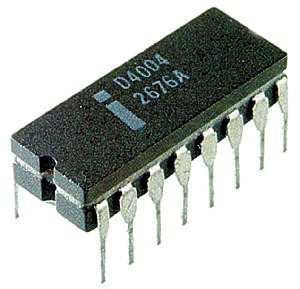
\includegraphics[height=2cm]{../illustration/Intel4004.jpg}
\end{itemize}
\item Programmeur :
\begin{itemize}
\item Manipule un langage de plus haut niveau, plus convivial $\rightarrow$ $L_1$ \\

\includegraphics[height=2cm]{../illustration/evolution.jpg}
\end{itemize}
\end{itemize}
\end{frame}

\begin{frame}
\frametitle{Prise en charge des langages de haut niveau}
Deux méthodes de prise en charge :
\begin{itemize}
\item \textbf{Traduction} : 
\begin{itemize}
\item Remplacer chaque instruction de $L_1$ par une séquence d'instructions de $L_0$
\item Le programme obtenu est alors entièrement composé d'instructions du $L_0$
\end{itemize}

\item \textbf{Interprétation} : 
\begin{itemize}
\item Un langage écrit en $L_0$ prend en charge $L_1$ sous la forme d'un flux de donnée en entrée $\rightarrow$ \textbf{interpréteur}
\item Lecture séquentielle des instructions de $L_1$ et exécution des séquences $L_0$ correspondantes
\end{itemize}
\item \textit{Possibilité de combiner les des deux méthodes} \cite{tanen} 
\end{itemize}
\end{frame}

\begin{frame}
\frametitle{Empilement de machines virtuelles}
\begin{itemize}
\item Permet d'utiliser un langage de programmation $L_n$ très éloigné de $L_0$
\begin{itemize}
\item augmentation progressive de la complexité
\item couches successives de machines virtuelles, interprétant des langages de niveau d'abstraction croissant ($L_n \rightarrow L_{n-1}$)
\end{itemize}

\item Augmentation progressive du niveau d'abstraction
\begin{itemize}
\item machine physique exécute le langage $L_0$ 
\item machine virtuelle $M_1$ interprète le langage $L_1 \rightarrow L_0$
\item machine virtuelle $M_2$ interprète le langage $L_2 \rightarrow L_1$
\item ...
\item machine virtuelle $M_n$ interprète le langage $L_n \rightarrow L_{n-1}$
\begin{itemize}
\item interpréteur/traducteur de niveau n-1
\end{itemize}
\end{itemize}
\end{itemize}
\end{frame}

\begin{frame}
\frametitle{Empilement de machines virtuelles}
\begin{itemize}
\item Au minimum deux couches :
\begin{itemize}
\item Couche 1 : langage machine
\item Couche 0 : matériel (portes logiques, additionneur... )
\end{itemize}
\item Généralement 6 couches \cite{tanen} :
\begin{itemize}
\item Niveau 5 : couche langage orienté application
\item Niveau 4 : couche langage d'assemblage
\item Niveau 3 : couche système d'exploitation
\item Niveau 2 : couche architecture du jeu d'instructions (ISA\footnote{Instruction Set Architecture})
\item Niveau 1 : couche micro-architecture
\item Niveau 0 : couche circuits logiques
\end{itemize}
\end{itemize}
\end{frame}

\begin{frame}
\frametitle{Empilement de machines virtuelles}
\begin{itemize}
\item Niveaux 0 $\rightarrow$ 3 toujours interprétés
\item Niveaux 4 et supérieurs généralement traduits
\end{itemize}
\begin{block}{Matériel et logiciel sont logiquement équivalents}
Le matériel n'est que du logiciel pétrifié.

\textit{Karen Panetta Lentz}
\end{block}
\begin{itemize}
\item La réciproque est également vraie (émulation)
\item Problème du choix des fonctions à faire supporter par le matériel
\end{itemize}
\end{frame}


\begin{frame}
\frametitle{Le jeu d'instruction du processeur}
\begin{definition}
Le jeu d'instructions est l'ensemble des opérations qu'un processeur d'ordinateur peut exécuter.  \cite{wp-ji}

Ces circuits permettent d'effectuer des opérations :
\begin{itemize}
\item élémentaires
\begin{itemize}
\item addition, ET/OU logique...
\item chargement, rangement…
\end{itemize}

\item plus complexes\begin{itemize}
\item instructions SIMD\footnote{Single instruction multiple data}…
\end{itemize}
\end{itemize}
\end{definition}

\end{frame}

\begin{frame}
\frametitle{RISC contre CISC}
\begin{itemize}
\item Premiers processeurs
\begin{itemize}
\item faible nombre d'instructions
\end{itemize}
\item Complexification progressive $\rightarrow$ \textbf{CISC}
\begin{itemize}
\item haut niveau d'abstraction
\item certaines instructions nécessitent plusieurs cycles
\item nombre d'instructions figé (cas du VAX de DEC, Z80), sauf en cas d'utilisation d'un interpréteur
\end{itemize}
\item Limitation du jeu d'instruction $\rightarrow$ \textbf{RISC}
\begin{itemize}
\item Instruction simples et rapides
\item 50 instructions optimisées (contre 200 - 300 pour le VAX)
\item limitation du niveau de complexité des adressages
\item augmentation du nombre de registres
\end{itemize}
\end{itemize}
\end{frame}

\begin{frame}
\frametitle{RISC contre CISC}
\begin{itemize}
\item Le RISC pur n'a pas réussi à s'imposer dans la micro-informatique
\begin{itemize}
\item échec relatif des UltraSPARC de Sun, PowerPC d'IBM
\item épineux problème de la rétro-compatibilité
\item décollage des ARM\footnote{Advanced Risc Machine} sur nouvelles plateformes
\end{itemize}
\item Le CISC reste encore la règle
\item Principes de conception RISC $\rightarrow$ processeurs CISC
\end{itemize}
\begin{exampleblock}{Cas du 486 d'Intel \cite{wp-apix86}}
\begin{itemize}
\item Propose un CISC
\item Cœur RISC $\rightarrow$  instructions les plus simples et fréquentes
\item Interpréteur $\rightarrow$ instructions plus complexes (lentes)
\begin{itemize}
\item micro-instructions
\end{itemize}
\end{itemize}
\end{exampleblock}
\end{frame}

\begin{frame}{Processeurs CISC/RISC}
\begin{columns}
\column{.5\textwidth}
\begin{exampleblock}{Processeurs CISC}
\begin{itemize}
\item S/360 (IBM)
\item VAX (DEC)
\item 68xx, 680x0 (Motorola)
\item x86, Pentium (Intel)
\end{itemize}

\end{exampleblock}
\column{.5\textwidth}
\begin{exampleblock}{Processeurs RISC}
\begin{itemize}
\item Alpha (DEC)
\item PowerPC (Motorola)
\item MIPS
\item PA-RISC (Hewlett-Packard)
\item SPARC
\item ARM 
\end{itemize}
\end{exampleblock}
\end{columns}
\begin{center}
L'optimisation du code par les compilateurs est plus simple pour les processeurs RISC que pour les processeurs CISC
\end{center}
\end{frame}



%------------------------------------------------------------------- 
\subsection{Chaîne de production des programmes}
%------------------------------------------------------------------- 
\begin{frame}
\frametitle{Chaîne de production des programmes}
\begin{itemize}
\item Compilateurs, assembleurs, interpréteurs
\item Traduction en langage machine
\item Éditeur de lien
\item Assemblage de modules
\item Chargeur
\item Mise en mémoire d’un exécutable
\item Débogueur
\begin{itemize}
\item Facilite le test des programmes
\end{itemize}
\end{itemize}
\end{frame}


\begin{frame}
\frametitle{Production d'un programme}
Cas d'un programme écrit en langage C
\begin{itemize}
\item \textbf{Compilé} en assembleur
\item \textbf{Assemblé} en module objet (langage machine)
\begin{itemize}
\item Peuvent faire partie de bibliothèques
\item Appel aux bibliothèques : point de branchement
\end{itemize}
\item \textbf{Lié} en image binaire
\begin{itemize}
\item Édition de liens statique
\item Édition de liens dynamique
\end{itemize}
\item \textbf{Chargé} en mémoire pour exécution
\end{itemize}
\end{frame}

\begin{frame}
\frametitle{Le langage assembleur \cite{wp-assembleur}}
\begin{definition}
Un langage d'assemblage ou "langage assembleur" est, en programmation informatique, un langage de bas niveau qui représente le langage machine sous une forme lisible par un humain.
\end{definition}
\begin{itemize}
\item Combinaisons de bits $\rightarrow$ symboles « mnémoniques »
\item Origines : \begin{itemize}
\item Programmes de l'EDSAC (1949) - traduction manuelle
\item Premier assembleur écrit par Nathaniel Rochester pour l'IBM-701 (premier IBM commercialisé) en 1954
\end{itemize}
\item Supplanté par les langages de haut niveau (FORTRAN, COBOL, PL/I... ) en 1970-1980
\end{itemize}

\end{frame}

\begin{frame}
\frametitle{Le rôle du compilateur}
\begin{block}{Tâche principale d'un compilateur}
Produire un code objet correct qui s'exécutera sur un ordinateur, à partir d'un code exprimé dans un langage de plus haut niveau.
\end{block}
Autres fonctions courantes :
\begin{itemize}
\item Optimiser le code généré
\item Améliorer la vitesse d'exécution
\item Réduire l'occupation mémoire du programme
\end{itemize}
\end{frame}

\begin{frame}
\frametitle{Les trois parties d'un compilateur \cite{wp-compilateur}}
\begin{itemize}
\item <1-> Partie \textbf{avant} (ou frontale, souche) :
\begin{itemize}
\item Préprocesseur
\item Lecture du code source
\item Production de la représentation intermédiaire
\item Indépendante du code cible
\end{itemize}

\item <2-> Partie \textbf{centrale} (facultative)
\begin{itemize}
\item Optimisation du code intermédiaire
\item Indépendante des langages source et cible
\end{itemize}

\item <3-> Partie \textbf{arrière} (ou finale)
\begin{itemize}
\item Exploite la représentation intermédiaire
\item Produit le code cible
\item Indépendante du code source
\end{itemize}
\end{itemize}
\end{frame}


\begin{frame}{Les quatre étapes de la production d'un exécutable}
\begin{itemize}
\item <1-> [Etape 1] Le \textbf{prétraitement} (preprocessing) : traite les directives de compilation et les macros (commencent par \#)
\item <2-> [Etape 2] La \textbf{compilation} (ccl) : produit du code assembleur (spécifique à une architecture donnée)
\item <3-> [Etape 3] L'\textbf{assemblage} (as) : produit un fichier objet à partir du code assembleur
	\begin{itemize}
	\item Unix récents $\rightarrow$ format ELF (Executable and Linking Format)
	\item Depuis Windows NT $\rightarrow$ format PE32/64 (Portable Executable). Remplace NE (New Executable File Format)
	\end{itemize}
\item <4> [Etape 4] L'\textbf{édition de lien} : fait le lien entre les différentes fonctions utilisées dans les fichiers objets.

Génération de l'exécutable.
\end{itemize}
\end{frame}

\begin{frame}
\frametitle{La chaîne de production d'un programme}
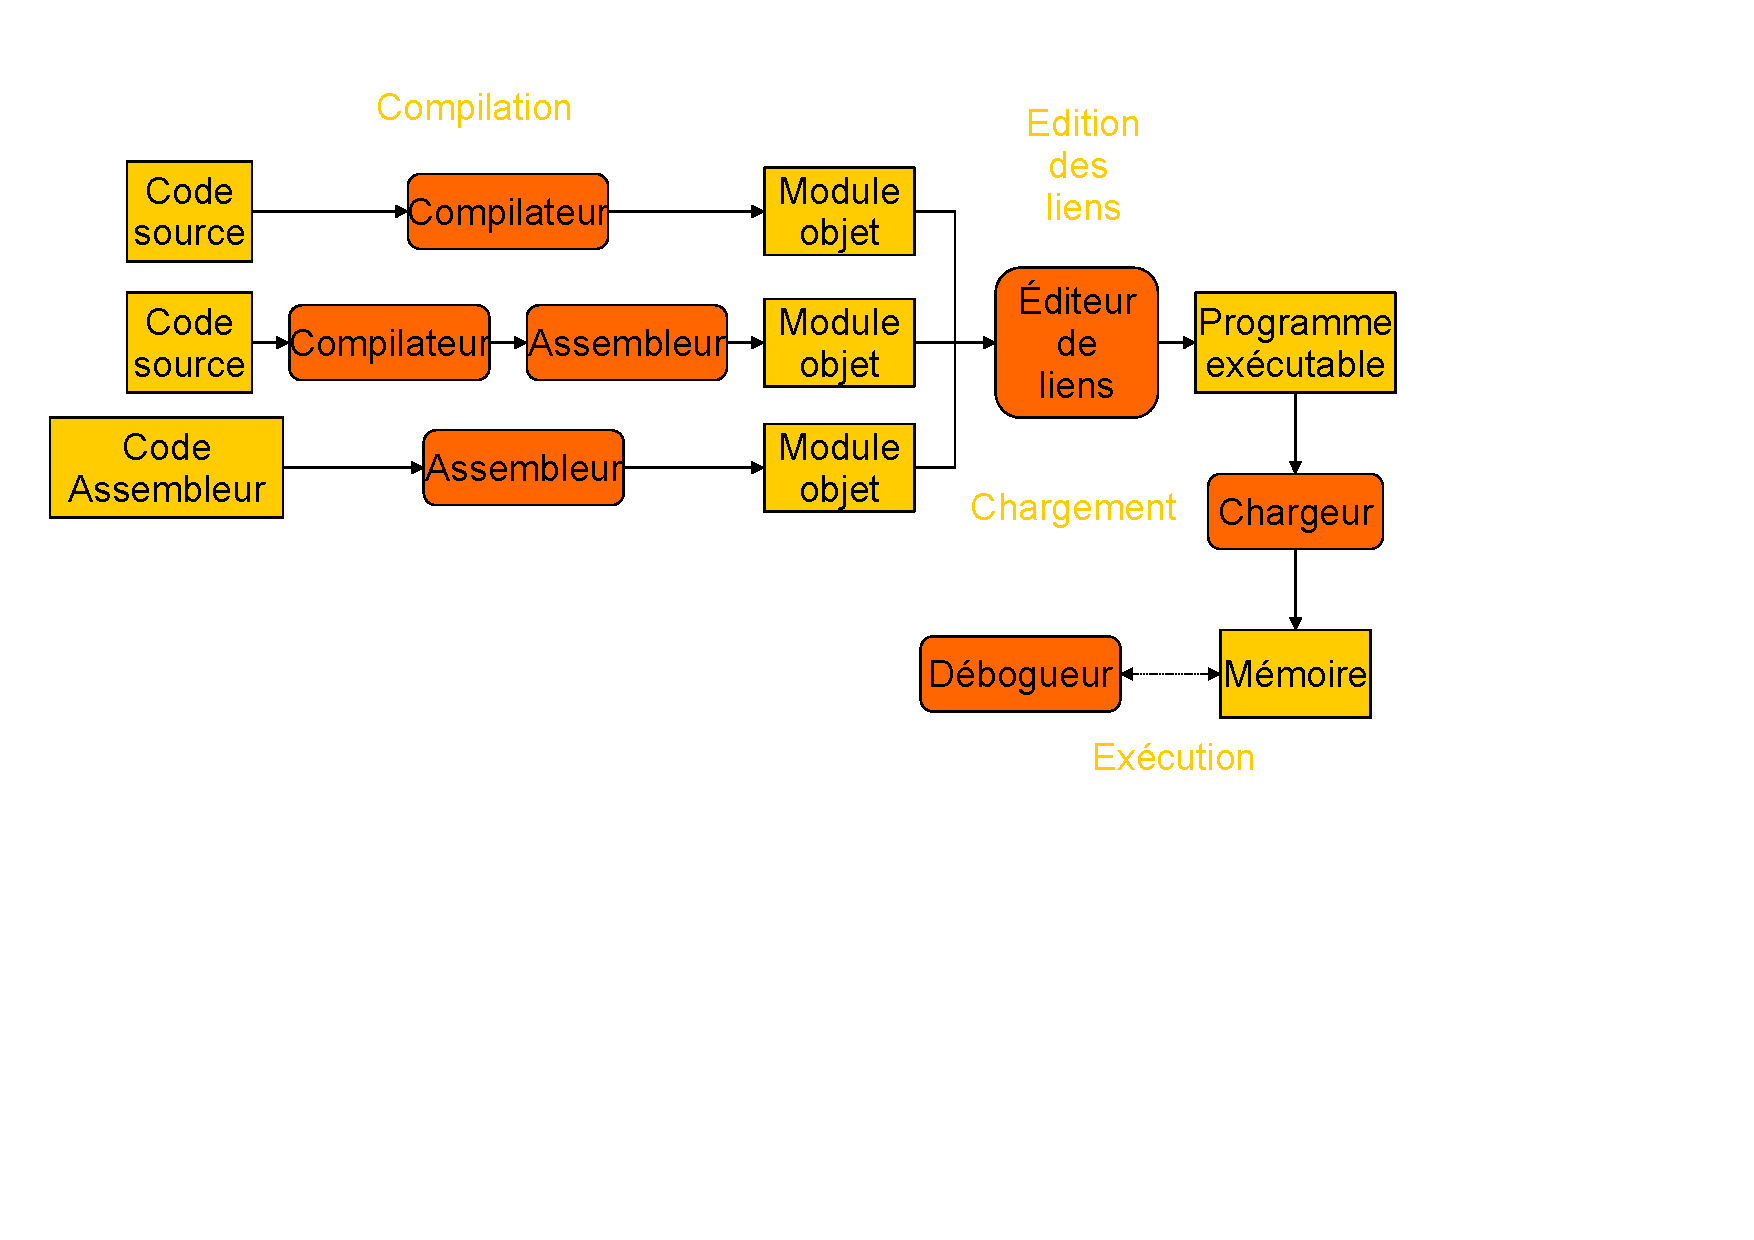
\includegraphics[width=\textwidth]{../illustration/chaine_prod_pgm.pdf}
\end{frame}


\begin{frame}
\frametitle{Compilateur croisé (\textit{Cross Compiler})}

\begin{block}{Qu'est-ce qu'un compilateur croisé ?}
C'est un programme capable de traduire un code source en code objet destiné à un environnement d'exécution différent de celui où la compilation est effectuée.
\end{block}

\begin{exampleblock}{Exemples}
\begin{itemize}
\item Compilation sur x86 d'un exécutable pour ARM ou PPC
\item Optimisation spécifiques au type de processeur
\end{itemize}
\end{exampleblock}
Souvent utilisé dans le domaine de l'embarqué
\begin{itemize}
\item limitations de l'architecture cible
\end{itemize}
\end{frame}

\begin{frame}
\frametitle{Exemple : le compilateur GCC}
\begin{itemize}
\item \textbf{Gnu Compiler Collection}
\item Supporte de nombreux langages sources
\begin{itemize}
\item C, C++, ObjectiveC, Java, Ada, Fortran, Pascal, VHDL, D, Go, Modula, PL/1, OpenMP
\end{itemize}
\item Peut générer des objets pour de nombreuses plateformes
\begin{itemize}
\item Types de microprocesseurs
\begin{itemize}
\item x86, ARM, PowerPC, DEC Alpha, MIPS, SPARC...
\end{itemize}
\item Systèmes d'exploitation
\begin{itemize}
\item Windows, Linux, MacOS, VMS...
\end{itemize}
\end{itemize}
\item Porté sur de nombreuses plateformes
\item Explique en grande partie la grande portabilité des applications GNU
\end{itemize}
\end{frame}


\begin{frame}{Exemple de compilation croisée avec GCC}
\begin{exampleblock}{Connaitre le nom de l'architecture de compilation}
\texttt{\$ gcc -dumpmachine}

\texttt{i686-linux-gnu}
\end{exampleblock}

\begin{exampleblock}{Compilation pour processeur ARM depuis i686}
\texttt{\$ arm-linux-gnuabi-gcc essai.c -o essai}
\end{exampleblock}

\begin{exampleblock}{Compilation pour Windows depuis Linux}
\texttt{\$ i586-mingw32msvc-gcc essai.c -o essai.exe}
\end{exampleblock}
\end{frame}

\begin{frame}{Compilation et debug avec GCC}
\begin{exampleblock}{Générer du code assembleur avec debug}
\texttt{\$ gcc -S -g3 source.c}
\begin{itemize}
\item \texttt{-S} : compilation seule (génération code assembleur)
\item \texttt{-g3} : intégration des codes de debug (maximal debug information) 
\end{itemize}
$\rightarrow$ Génération d'un fichier \texttt{source.s}, contenant le code assembleur
\end{exampleblock}

\begin{table}[htdp]
\begin{center}
\begin{tabular}{|c|c|}
\hline
Option&Description\\
\hline
\texttt{-g0} & No debug information \\
\texttt{-g1} & Minimal debug information \\
\texttt{-g} & Default debug information \\
\texttt{-g3} & Maximal debug information \\
\hline
\end{tabular}
\end{center}
\end{table}

\end{frame}



\begin{frame}
\frametitle{Compilateur \textit{bootstrap}}
\begin{block}{Qu'est-ce que le bootstraping ?}
En informatique, le terme \emph{bootstrapping} décrit les techniques nécessaires à l'écriture d'un compilateur (ou d'un assembleur) dans le langage de programmation cible qu'il doit compiler
\end{block}

\begin{columns}
\column{.6\textwidth}
\begin{itemize}
\item Les compilateurs sont généralement écrits avec le langage qu'ils compilent
\item Étape importante dans l'évolution d'un langage
\end{itemize}
\column{.4\textwidth}
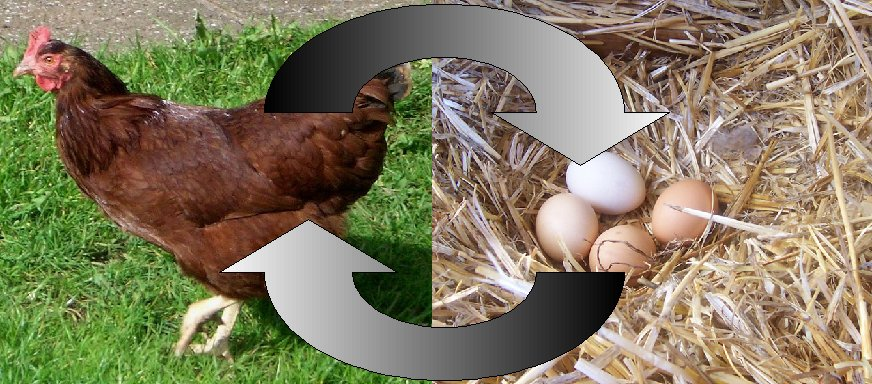
\includegraphics[height=2cm]{../illustration/Chickenegg.jpg}
\end{columns}
\end{frame}




\subsection{Edition de liens statique / dynamique}

\begin{frame}
\frametitle{Liaison dynamique et bibliothèques partagées}
\begin{itemize}
\item Édition de liens statique : 
\begin{itemize}
\item liaison de toutes les bibliothèques dans le fichier exécutable 
\begin{itemize}
\item exécutable monolithique
\end{itemize}

\end{itemize}
\item <2->Édition de liens dynamique :
\begin{itemize}
\item liaison et chargement reportés au plus tard
\begin{itemize}
\item au moment de l'exécution
\end{itemize}
\item évite duplication des bibliothèques
\begin{itemize}
\item bibliothèques partagées
\end{itemize}
\item ne charge que le strict nécessaire
\end{itemize}
\end{itemize}
\end{frame}


\begin{frame}
\frametitle{Liaison dynamique et bibliothèques partagées}
\begin{itemize}
\item Stub :
\begin{itemize}
\item Élément de remplacement (pointeur)
\item Inséré dans l'image, à la place d'une référence à la bibliothèque (indication de la version)
\item Vérifie la présence de la routine utilisée en mémoire et la charge si besoin
\end{itemize}
\item Assistance de la part du système
\begin{itemize}
\item Permet à plusieurs processus d'accéder aux mêmes bibliothèques partagées
\end{itemize}
\end{itemize}
\end{frame}


\subsection{Exemple des “shared object” de Linux}

\begin{frame}{Les “shared object” de Linux}
\begin{itemize}
\item Partage d'objets entre programmes
\begin{itemize}
\item Plus évolué que le simple partage de mémoire
\item Partage données et fonctions
\item Mécanismes de synchronisation
\end{itemize}
\item Peut être chargé et déchargé dynamiquement
\begin{itemize}
\item Format ELF
\item Mécanisme de chargement et de liaison dynamique
\item Utilisé par le noyau $\rightarrow$  modules
\end{itemize}
\item Utilisation :
\begin{itemize}
\item Stockées dans les répertoires \texttt{/lib/}, \texttt{/usr/lib/}...
\item Resencement des bibliothèques existantes : \texttt{ldconfig}
\item Consultation liaisons dynamiques d'un exécutable : \texttt{ldd}
\end{itemize}
\end{itemize}
\end{frame}

\subsection{Pile d'exécution}

\begin{frame}
\frametitle{Pourquoi une pile d'exécution ?}
\begin{itemize}
\item Le CPU exécute séquentiellement les instructions du programme
\item Lors d'un appel de fonction, l'exécution est transférée vers cette dernière (saut)
\begin{itemize}
\item Les appels de fonctions peuvent être imbriqués ou récursifs
\end{itemize}
\item Après avoir exécuté la fonction $\rightarrow$ retour au point d'appel (valeurs retour)
\end{itemize}
\begin{block}{Questions}
\begin{itemize}
\item Comment s'y retrouver dans les appels de fonctions ?
\item Comment retrouver les valeurs retour
\end{itemize}

\end{block}
\end{frame}

\begin{frame}
\frametitle{Pile d'exécution («la pile», «call stack»)}
\begin{block}{Finalités de la pile d'exécution}
Enregistrer des informations sur les fonctions actives 
\begin{itemize}
\item Trace de l'endroit où chaque fonction active doit retourner à la fin de son exécution
\item Valeurs retour des fonctions
\item Variables locales, paramètres de la fonction, etc...
\end{itemize}
\end{block}
\end{frame}

\begin{frame}
\frametitle{Pile d'exécution («la pile», «call stack»)}
\begin{itemize}
\item Structure de pile :
\begin{itemize}
\item FILO : First In Last Out
\item Restauration dans l'ordre inverse de la sauvegarde
\end{itemize}

\item <2->Manipulée par les langages d'assemblage
\item <2->Contenu de la pile cachée aux langages de haut niveau
\begin{tabbing}
Implémentation \= mise en œuvre par le compilateur \\
\> contrainte par l'architecture matérielle \\ \>(CPU, mémoire... )
\end{tabbing}
\end{itemize}
\end{frame}


\begin{frame}
\frametitle{Exemple d'utilisation d'une pile d'exécution}
\begin{columns}
\column<1-2>{.62\textwidth}
\begin{block}{Code source}
\tiny{\verbatiminput{include/pile.c}}
\end{block}
\column<2>{.38\textwidth}
\begin{exampleblock}{Résultat}
\tiny{\verbatiminput{include/pile.txt}}
\end{exampleblock}
\end{columns}
\end{frame}

\begin{frame}{Exemple d'utilisation d'une pile d'exécution}
\begin{columns}
\column{.5\textwidth}
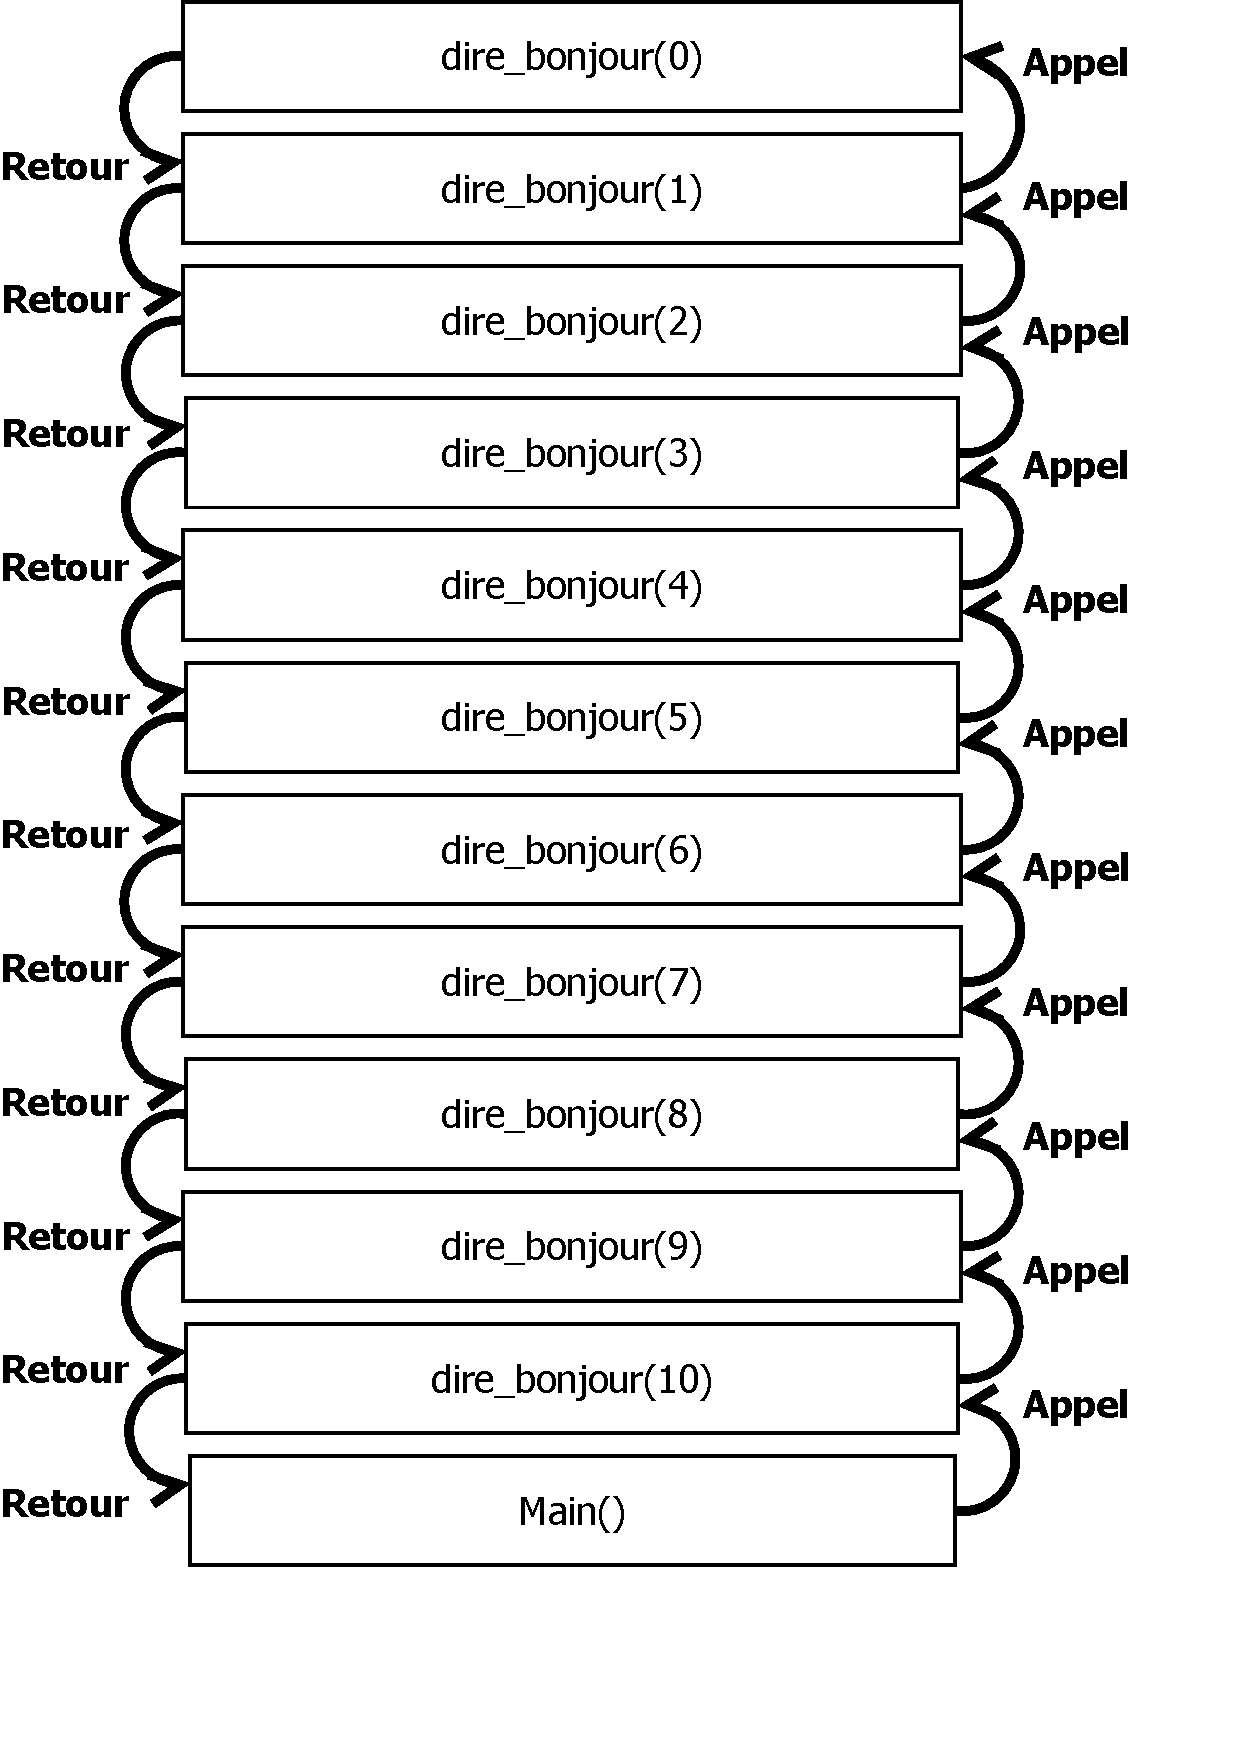
\includegraphics[height=\textheight]{../illustration/PileAppel.pdf}
\column{.5\textwidth}
\begin{exampleblock}{Résultat}
\tiny{\verbatiminput{include/pile.txt}}
\end{exampleblock}
\end{columns}
\end{frame}



\frame[allowframebreaks]
{
\frametitle{Bibliographie}
\bibliographystyle{plain}
\bibliography{include/smb137}
}

\end{document}

